\subsection{A small bump}
On June 2nd 2015, the day before CMS recorded its first ever 13 TeV event, a pre-print appeared on the arXiv "Search for high-mass diboson resonances with boson-tagged jets in proton-proton collisions at $\sqrt{s} = 8$ \TeV with the ATLAS detector"~\cite{Aad2015}.
It was an analysis of the full ATLAS Run 1 dataset, corresponding to 20.3 \fbinv, searching for heavy resonances decaying to vector bosons in the all-hadronic state. The analysis documented a 3.4 $\sigma$ excess for a heavy resonance decaying to \PW\PZ around 2 \TeV.
The corresponding CMS analysis, published the previous year, had a 1.3 $\sigma$ excess at roughly the same resonance mass, but mostly compatible with a \PW\PW final state hypothesis~\cite{Khachatryan:1700394}. Figure~\ref{fig:searchI:8tev} shows the corresponding dijet invariant mass spectrum as seen by ATLAS (left) and the upper limit on the production times the cross section for a $G_{Bulk}$ decaying to \PW\PW (right)  as documented by CMS.

\begin{figure}[ht] 
    \centering
    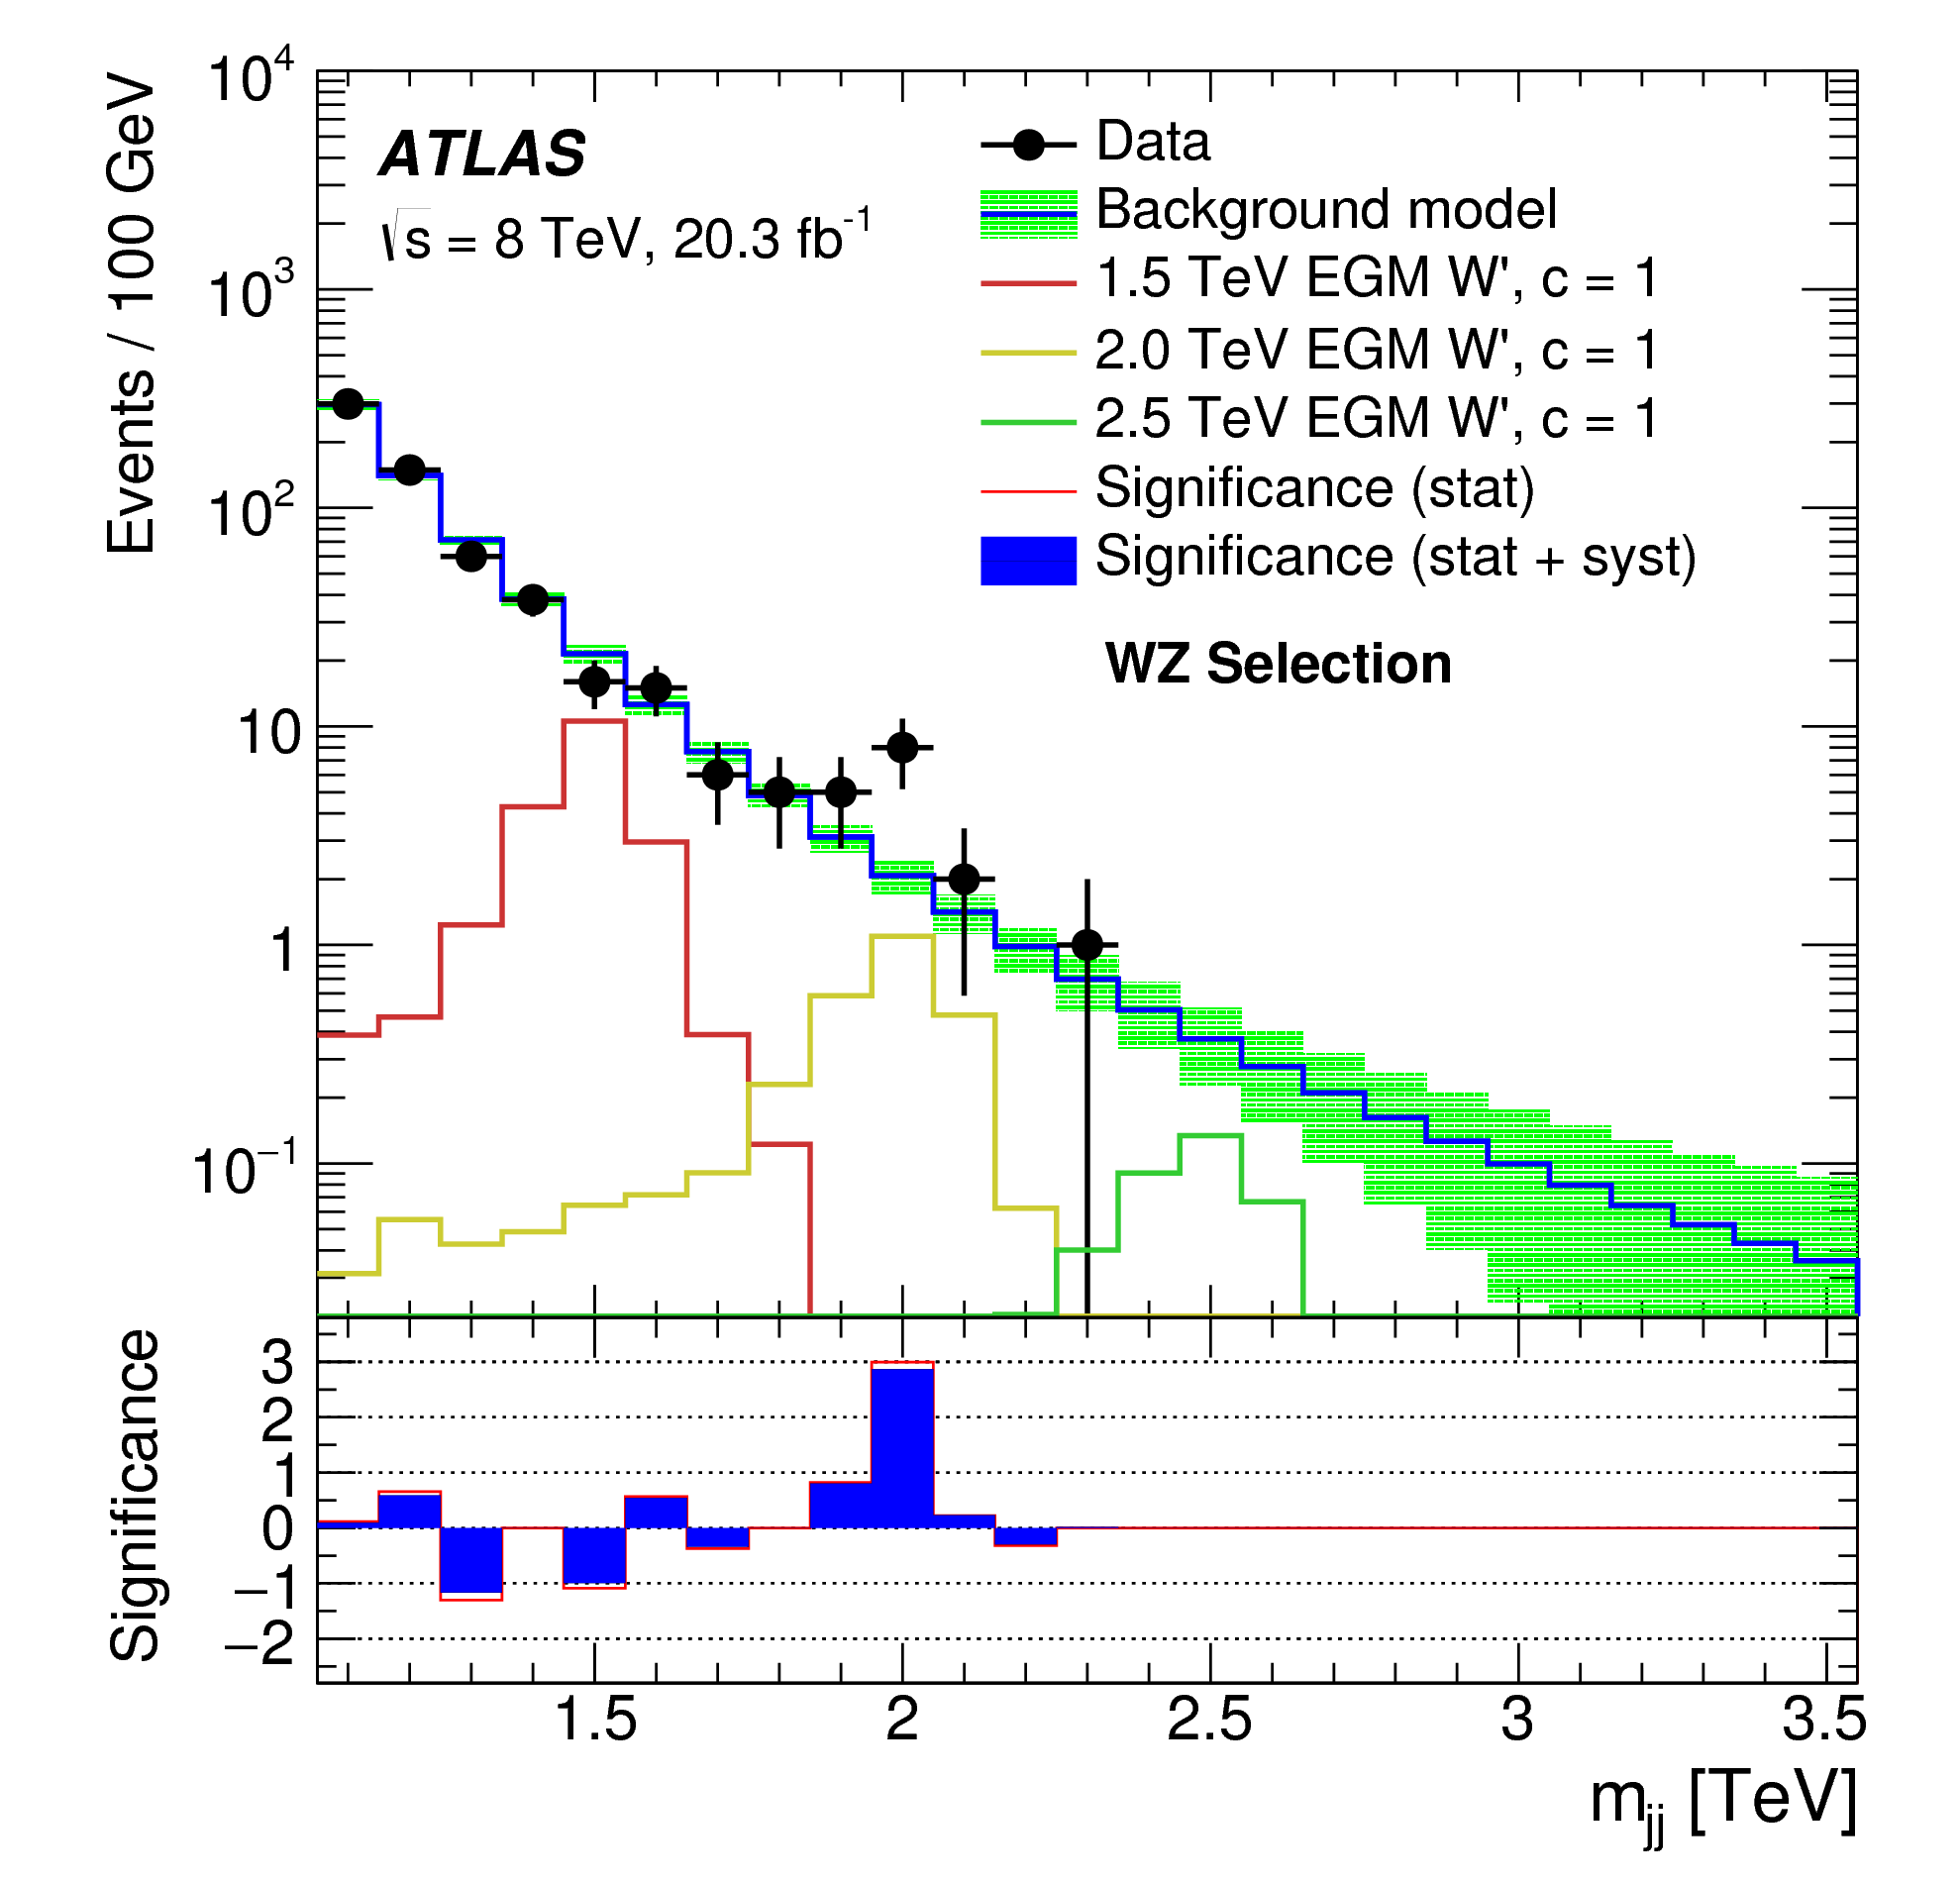
\includegraphics[width=0.4\textwidth]{figures/analysis/search1/misc/atlas_8tev.png}
    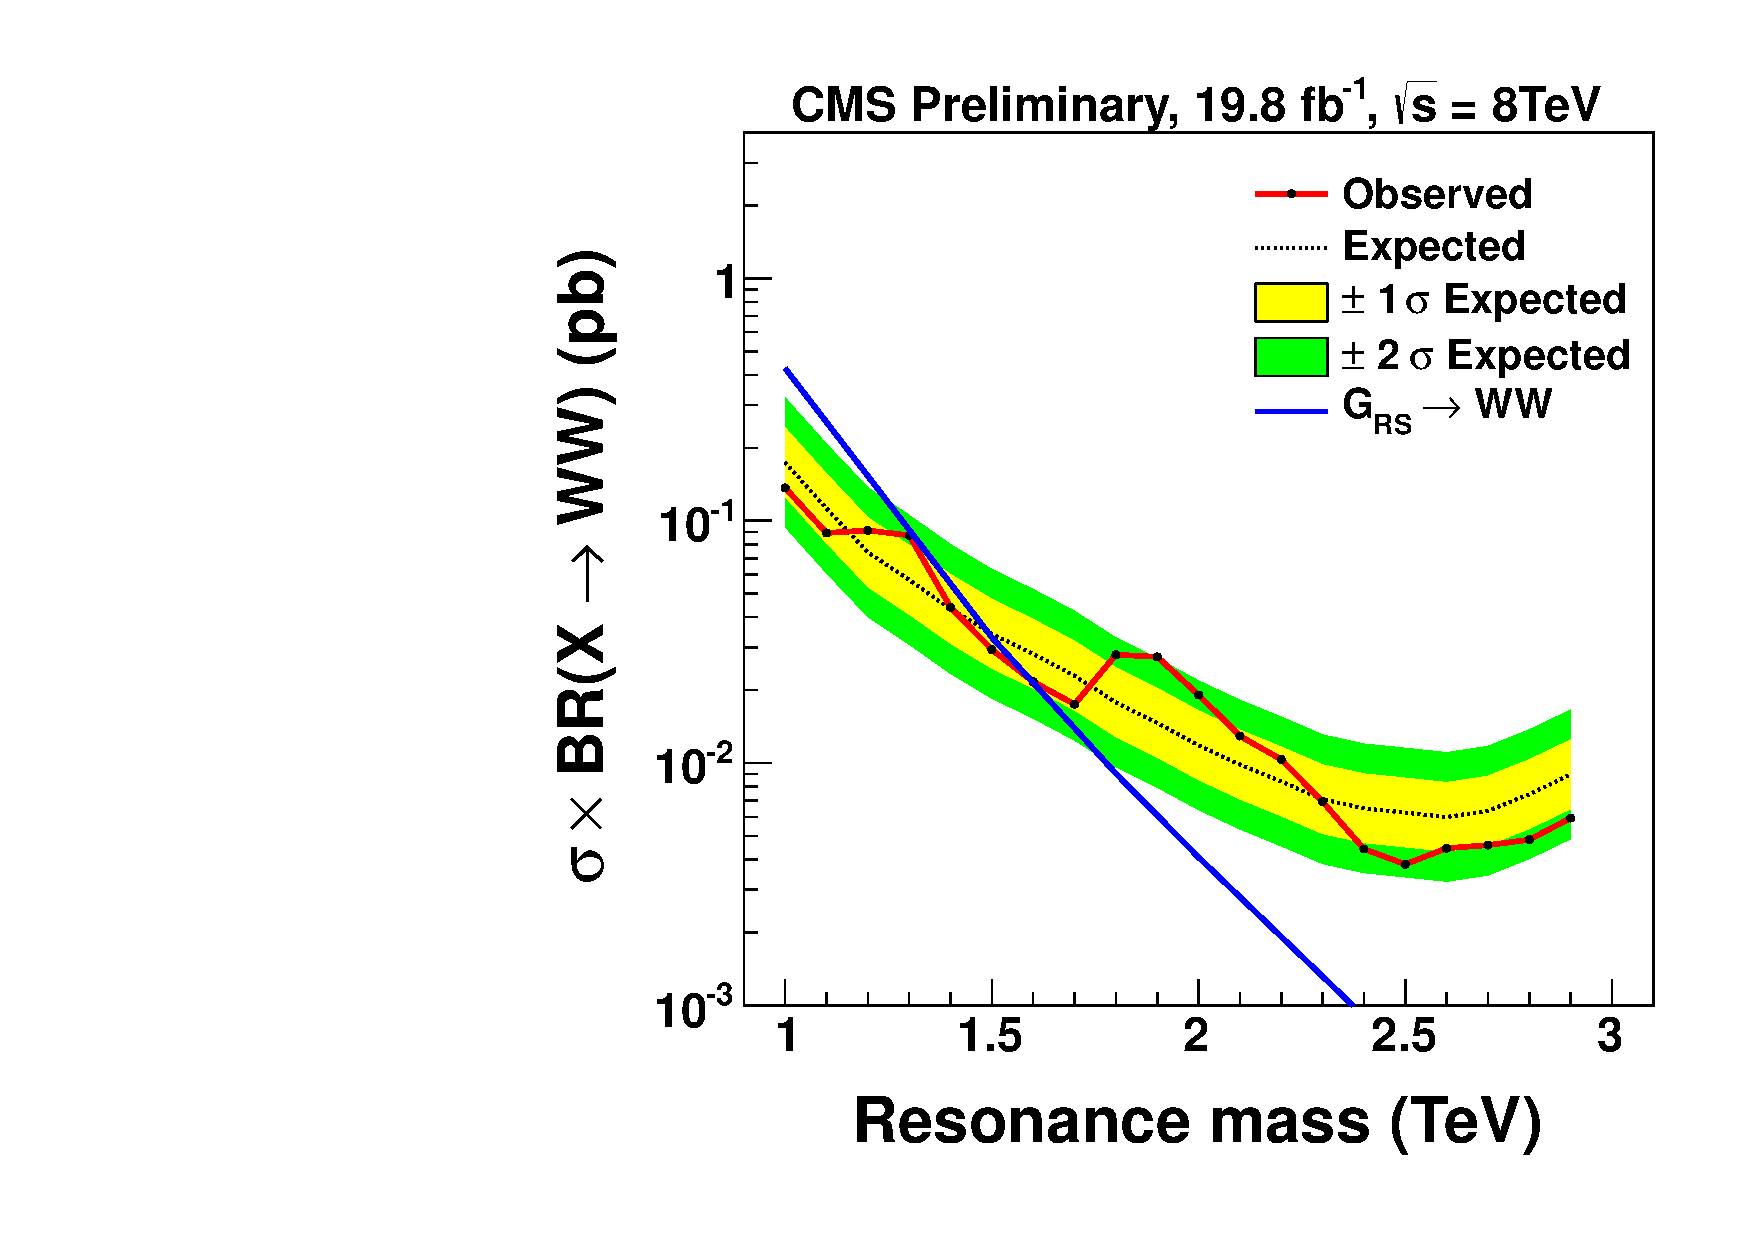
\includegraphics[width=0.4\textwidth]{figures/analysis/search1/misc/EXO-12-024_gWW.pdf}
    \caption{The mass (top) and \PT (bottom) resolution comparing PF only (blue), PF+CHS (red) and PUPPI (pink) jets. The absolute resolution (left) as well as the resolution as a function of the number of reconstructed primary vertices in the event (right)is shown~\cite{Bertolini2014}.}
    \label{fig:searchI:8tev}
\end{figure}

The two measurements were found to be compatible, favoring a heavy resonance with a production cross section of around 5 \fbinv and a mass between 1.9 and 2.0 TeV decaying to either \PW\PW, \PW\PZ or \PZ\PZ~\cite{Dias:2015mhm}. Figure~\ref{fig:searchI:8tevcombo} show the obtained p-value of the ATLAS (red) and CMS (blue) search as well as their combination (black).  

\begin{figure}[ht] 
    \centering
    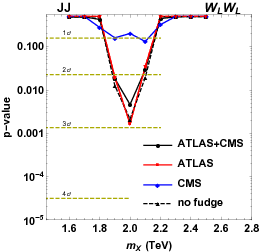
\includegraphics[width=0.25\textwidth]{figures/analysis/search1/misc/CMS_ATLAS_BulkWW_JJ_dijetfit_p.png}
    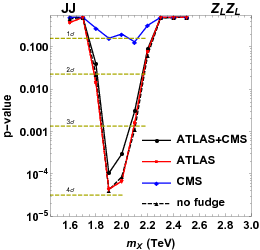
\includegraphics[width=0.25\textwidth]{figures/analysis/search1/misc/CMS_ATLAS_BulkZZ_JJ_dijetfit_p.png}
    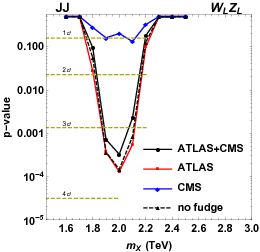
\includegraphics[width=0.25\textwidth]{figures/analysis/search1/misc/CMS_ATLAS_WZ_JJ_dijetfit_p.png}
    \caption{p-values as a function of resonance mass obtained with an emulation of the ATLAS (red) and CMS (blue) searches as well as the combination of the two (black). Here for a \PW\PW (left), \PW\PZ (middle) and \PZ\PZ (right) hypothesis~\cite{Dias:2015mhm}.}
    \label{fig:searchI:8tevcombo}
\end{figure}

The combination of the two excesses and the timing of the ATLAS paper, naturally lead to some excitement and in the coming weeks, the arXiv was flooded with theory papers seeking an explanation for the measurements.
The pressure on seeing early results with 13 TeV data in the VV all-hadronic final state was high, and it was agreed with CMS Physics Coordination that a preliminary analysis would be ready in December that same year, only 6 months after the first 13 TeV collision.

\subsection{Analysis strategy}

When a resonance X with a mass above 1 TeV decays into a vector boson pair, the bosons have a very high energy ($\tilde\PT=\mX/2=500 \GeV$, assuming X is produced at rest). The boson is co-called "boosted". The decay products of a hadronically decaying boosted vector boson, will therefore not appear as back-to-back in the lab frame but rather be very collimated, as described in Section~\ref{sec:objreco:substructure}. This results in a final state with two large high-\PT jets, where an AK R=0.8 jet is expected to fully contain the two quarks coming from the vector boson decay. This is illustrated in Figure~\ref{fig:searchI:merged}.

\begin{figure}[ht] 
    \centering
    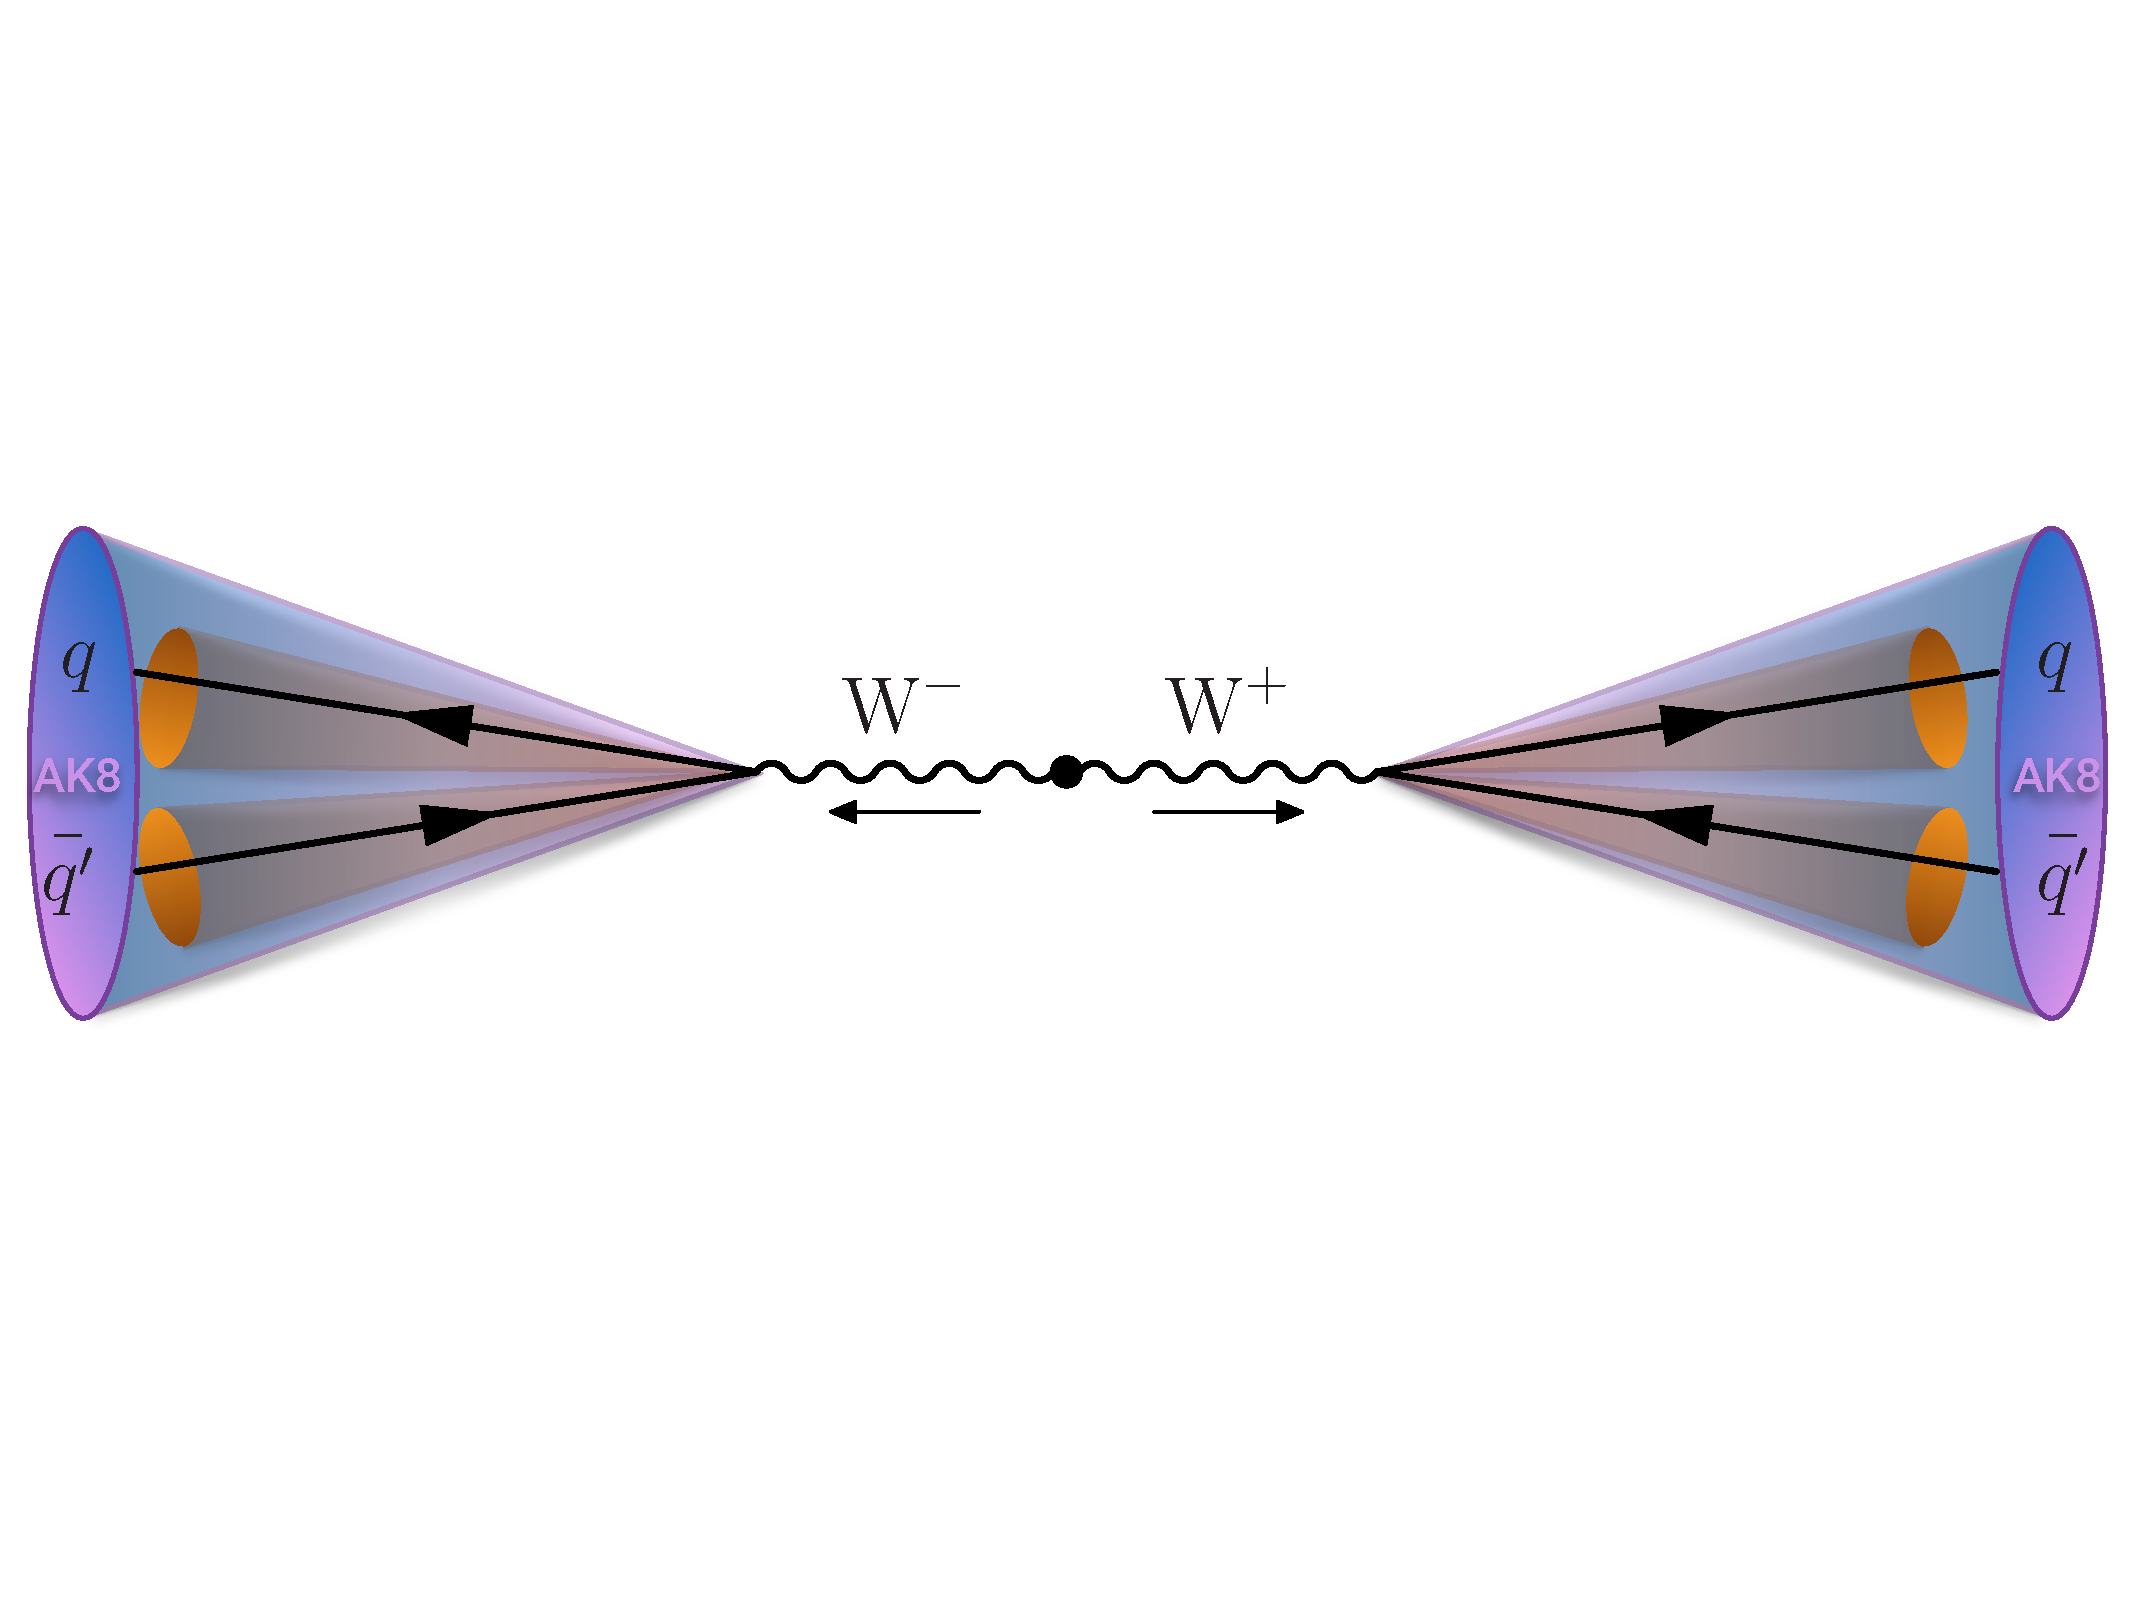
\includegraphics[width=0.70\textwidth]{figures/event_reconstruction/WWqqqq_merged_small.pdf}
    \caption{If a heavy ($>1 \TeV$) resonance decays into vector bosons, the transverse momentum of each boson will be large and its decay products are merged into one single large cone AK8 jet.}
    \label{fig:searchI:merged}
\end{figure}

The two jets are both expected to have a mass around the \PW of \PZ mass, and some intrinsic substructure stemming from their two-prong origin. The invariant mass of the dijet system, \mjj, should be roughly equal to the resonance mass \mX. This dijet system is the final state under scrutiny and the dijet invariant mass is the parameter of interest. Both \WW and \ZZ, as well as \WZ final states are of interest. \par

The main background for such an analysis, is QCD multijet events. As mentioned in Section~\ref{sec:objreco:substructure}, quark/gluon jets can obtain a high mass due to diffuse radiation and QCD processes have such a large cross section that the number of QCD jets with a mass compatible with the W mass can be large. In order to discriminate between the two, we take advantage of three properties: 1. The groomed mass of signal and background jets should be very different, 2. signal jets should appear two-prong like, quark/gluon jets not, and 3. the dijet invariant mass for a signal process should peak around the resonance mass while the QCD spectrum is predicted to be smoothly falling (we will get back to why this assumption is justified in Section~\ref{sec:searchI:bkg}). The strategy therefore consists of performing a smoothness test on \mjj of the observed data, a so-called "bump-hunt", by assuming that the signal will appear as a bump on top of a smooth distribution. This is illustrated in Figure~\ref{fig:searchI:bumphunt}.

\begin{figure}[ht] 
    \centering
    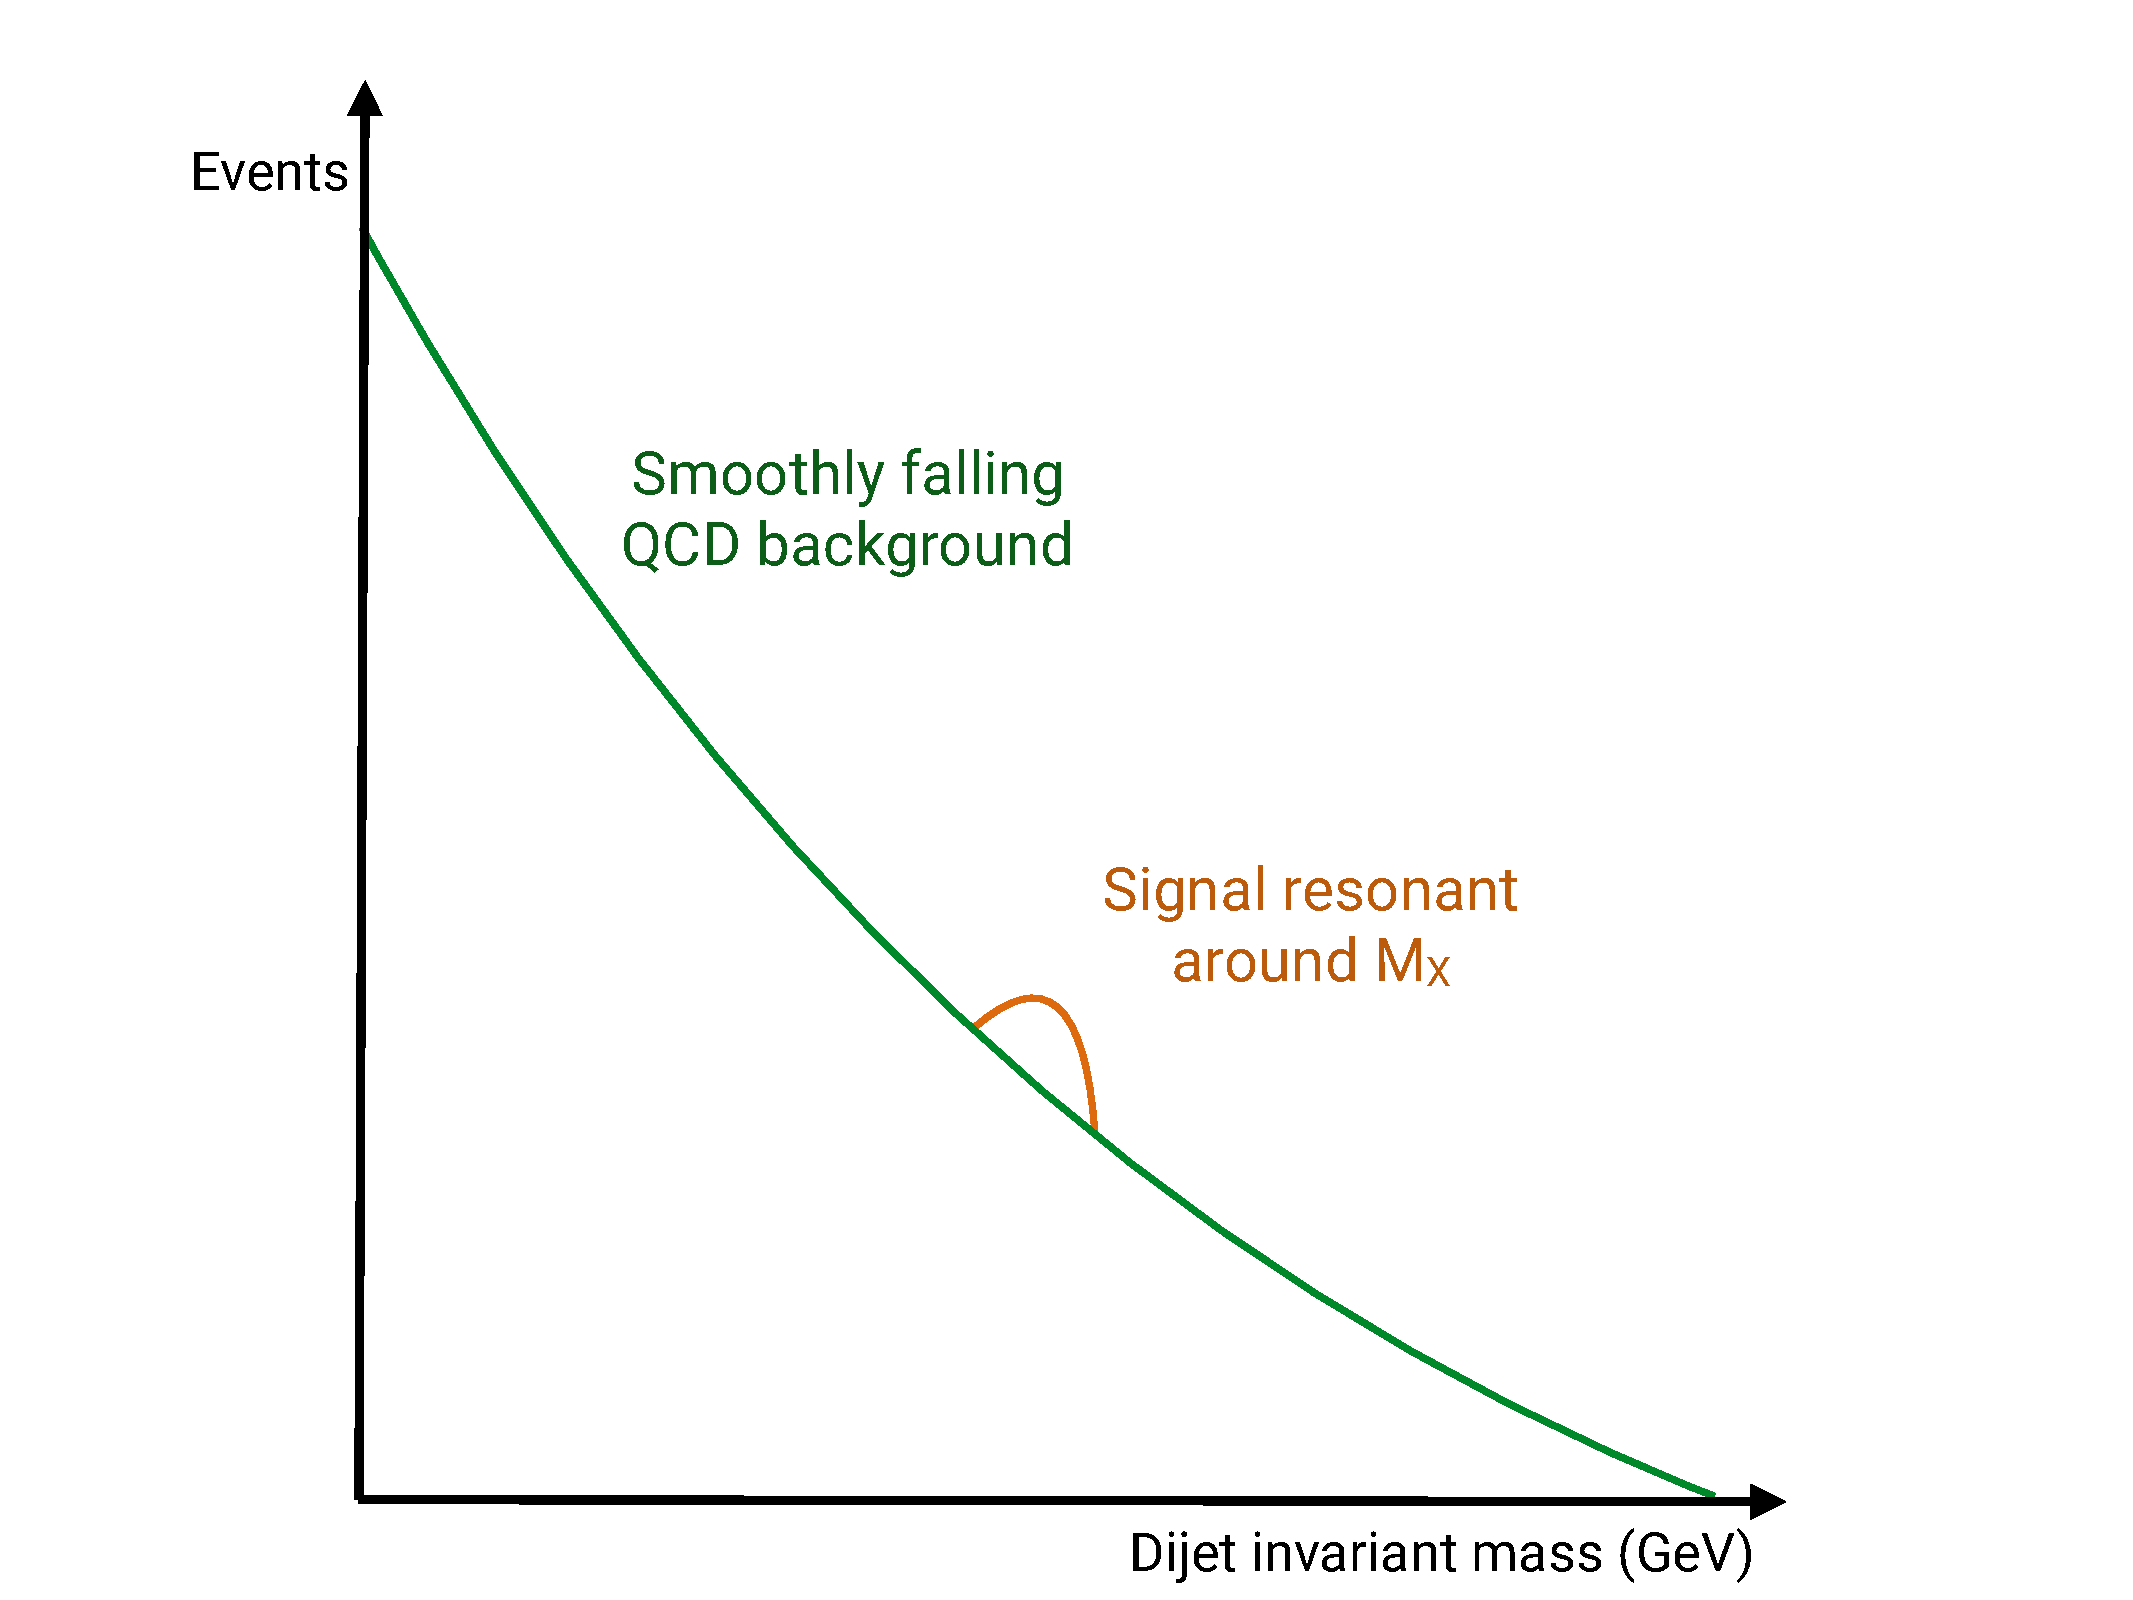
\includegraphics[width=0.49\textwidth]{figures/analysis/search1/misc/sigExtraction.pdf}
    \caption{The search strategy consists of looking for signal "bumps" in the dijet invariant mass on top of a smoothly falling QCD multijet background.}
    \label{fig:searchI:bumphunt}
\end{figure}

The benefit of such a method is that there is no need for any background simulation and the strategy is simple and robust. The disadvantage is that the analysis is intrinsically limited to regions where the dijet invariant mass spectrum is smooth, hence must avoid regions with continuities due to trigger turn-ons or kinematic selections.

\subsection{Data and simulated samples}
\label{sec:searchI:samples}
The data analyzed in this search correspond to a total integrated luminosity of 2.7\fbinv collected at a center-of mass energy of 13 \TeV between June and December 2015. The instantaneous luminosity of the LHC during this run was around half of the design luminosity ($0.5 \times 10^{34} \percms$), with an average number of primary vertices per event of $<\mu>=13$. \par\par

The bulk graviton model (see Section~\ref{sec:theory:wed}) and the HVT model (\PWpr{} and \PZpr{}, see Section~\ref{sec:theory:hvt}) are used as benchmark signal processes. In these models, the vector gauge bosons are produced with a longitudinal polarization in more than 99\% of the cases, which leads to a 24\% higher acceptance per boson for reasons explained in Section~\ref{sec:objreco:pol}. For the HVT model, a scenario (model B) with $g_{\rm V}=3$, $c_{\rm H}=-0.976243$, and $c_{\rm F}=1.02433$ is chosen, where the heavy resonance predominantly couple to bosons and the coupling to fermions is suppressed. The bulk graviton samples were generated with $\ktilde = 0.5$.
The resonance masses considered lie in the range 1.2 to 4\TeV and has a width of 0.1\% of the resonance mass. The narrow width allows us to neglect detector effect as the natural width of the resonance is smaller than the detector resolution, making the modeling of detector effects on the signal shape independent of the model. All signal samples are generated at leading order with \amcatnlo{} v2.2.2~\cite{Alwall:2014hca} \par\par

Simulated samples of the production of QCD multijet events are generated to leading order using \PYTHIA version 8.205~\cite{Sjostrand:2007gs} with the CUETP8M1 tune~\cite{Khachatryan:2015pea}.


\subsection{Event selection}

\subsubsection{Triggering}
\label{sec:searchI:trigger}
The first selection to be confronted in any analysis, is the trigger selection. Due to an overwhelming QCD background in all-hadronic final states, the threshold for fully-hadronic triggers is very large in order to keep the trigger rate low (preferably around 10-30 Hertz). In this analysis, we therefore decided to take advantage of triggers that place requirements on the jet groomed mass in addition to the "standard" triggers based on the scalar sum of jet transverse energy \HT. These "boosted" triggers were never before tested in data, and this analysis was the first published result taking advantage of grooming at the trigger level in CMS. The following \HT-based triggers (called inclusive triggers in the following) are used
\begin{itemize}
\item \texttt{HLT\_PFHT650\_WideJetMJJ900DEtaJJ1p5}
\item \texttt{HLT\_PFHT650\_WideJetMJJ950DEtaJJ1p5},
\item \texttt{HLT\_PFHT800}
\end{itemize}
where the two first triggers apply an additional cut on the $|\Delta \eta|$ between the two jets for reasons that will be explained below. In addition, two grooming triggers cutting on the jet trimmed mass (see Section~\ref{sec:objreco:trimming}) of 30 and 50 GeV are used
\begin{itemize}
\item \texttt{HLT\_AK8PFJet360\_TrimMass30}
\item \texttt{HLT\_AK8PFHT700\_TrimR0p1PT0p03Mass50}.
\end{itemize}
The tuneable parameters for the trimming algorithm at HLT are $r_{sub}=0.2$ and $p_{T,frac}=0.03$. The \texttt{HLT\_AK8PFJet360\_TrimMass30} trigger is seeded by single-object Level 1 triggers with jet $p_T$ thresholds of 176 or 200 GeV (\texttt{L1\_SingleJet176} or \texttt{L1\_SingleJet200}), and the remaining triggers requires an online \HT{}$>$150 or 175 GeV (\texttt{L1\_HTT150} or \texttt{L1\_HTT175}).\par

In order to avoid any kinks in the dijet invariant mass spectrum due to the presence of a trigger turn-on, we need to define for which dijet invariant mass the analysis triggers are fully efficient ($>99\%$), then cut away everything below that point.

In order to estimate the trigger efficiency, we use a lower threshold prescaled \HT{} trigger \texttt{HLT\_PFHT650} as reference trigger. This trigger has a prescale of 40, meaning it only stores information for every 40 events that trigger it, and is seeded by L1 triggers \texttt{L1\_HTT150} or \texttt{L1\_HTT175}. We then define the efficiency as
\begin{equation*}
\textrm{Efficiency} = \frac{N_{trigger+ref}}{N_{ref}}  
\end{equation*}
where $N_{trigger+ref}$ corresponds to events passing the trigger under study as well as the reference trigger and $N_{ref}$ corresponds to all events passing the reference trigger. Figure~\ref{fig:searchI:trigger-fits} shows the trigger turn-on curves as a function of dijet invariant mass for jets where one of the jets is required to have a pruned mass larger than 65 GeV (in other words, compatible with a W jet). A sharp turn-on for the inclusive triggers (top left) is observed, reaching the 100\% efficiency plateau for dijet masses of around 1.0--1.1 TeV. The grooming triggers, however, turn on more slowly and are not fully efficient before dijet invariant masses of around 1.2 TeV (top right). The real power of the grooming triggers become clear when adding them in OR with the \HT-based triggers. The bottom plot in Figure~\ref{fig:searchI:trigger-fits} compares the trigger turn-on curves as a function of dijet invariant mass for jets passing one of the three inclusive triggers only, one of the grooming triggers only and when combining all of them. Here, one can see that the 99\% efficiency threshold is lowered by 75 \GeV when including the substructure triggers, once substructure is required at analysis level.
This allowed for the analysis to start at a dijet invariant mass of 1 TeV.

\begin{figure}[h!]
\centering
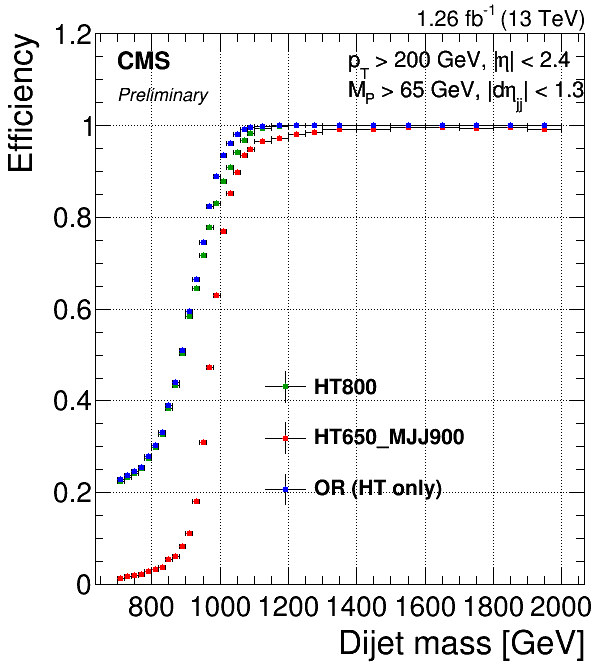
\includegraphics[width=0.4\textwidth]{figures/analysis/search1/AN-15-211//triggereffMjj-HT.png}
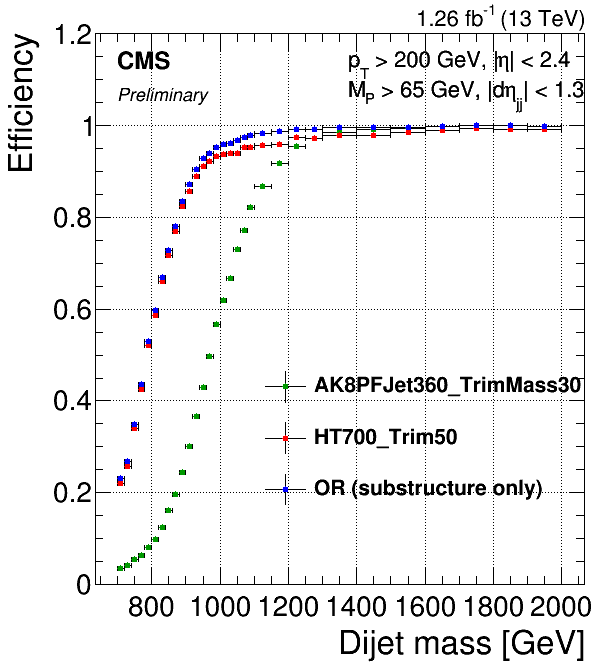
\includegraphics[width=0.4\textwidth]{figures/analysis/search1/AN-15-211//triggereffMjj-SUBST.png}\\
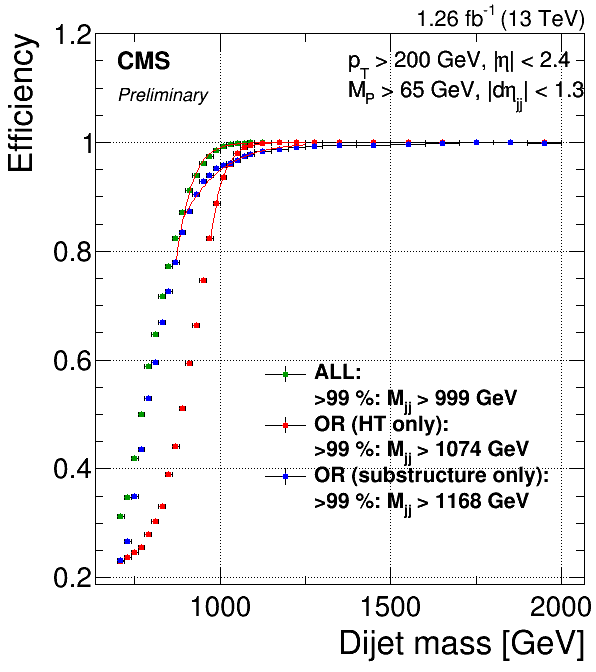
\includegraphics[width=0.4\textwidth]{figures/analysis/search1/AN-15-211/triggereffMjj-ALL.png}
\caption{Top: Efficiency for the inclusive triggers (top left) and the grooming triggers (top right) as a function of dijet invariant mass for jet pairs where one jet has a pruned mass larger than 65 GeV. Bottom: Comparison of trigger efficiencies for jets passing one of the HT-triggers only (red), for jets passing one of the grooming-triggers only (blue) and for jets passing one of the HT-triggers or one of the grooming triggers (green). Here as a function of dijet invariant mass for all jet pairs passing loose selections and where one jet has a pruned mass larger than 65 GeV. The 99\% efficiency threshold is lowered by 75 \GeV when including substructure taggers.}
\label{fig:searchI:trigger-fits}
\end{figure}


As a measure of the performance of the grooming triggers, we have in addition looked at the trigger efficiencies as a function of the offline groomed mass (pruned and softdrop, see Sections~\ref{sec:objreco:pruning} and ~\ref{sec:objreco:softdrop}), for the grooming trigger with the lowest mass threshold (30 \GeV). This is shown in Figure~\ref{fig:searchI:grooming-mj-trigger}, where an additional cut on the jet transverse momentum of one of the jets of 600 GeV is required and no other mass cut is applied. The trigger plateau is reached for offline groomed-jet masses around 50 GeV, an impressively sharp turn-on for a trigger paths first test i data (as reference trigger for this study, the prescaled trigger \texttt{HLT\_PFJet320} was used). 

\begin{figure}[h!]
\centering
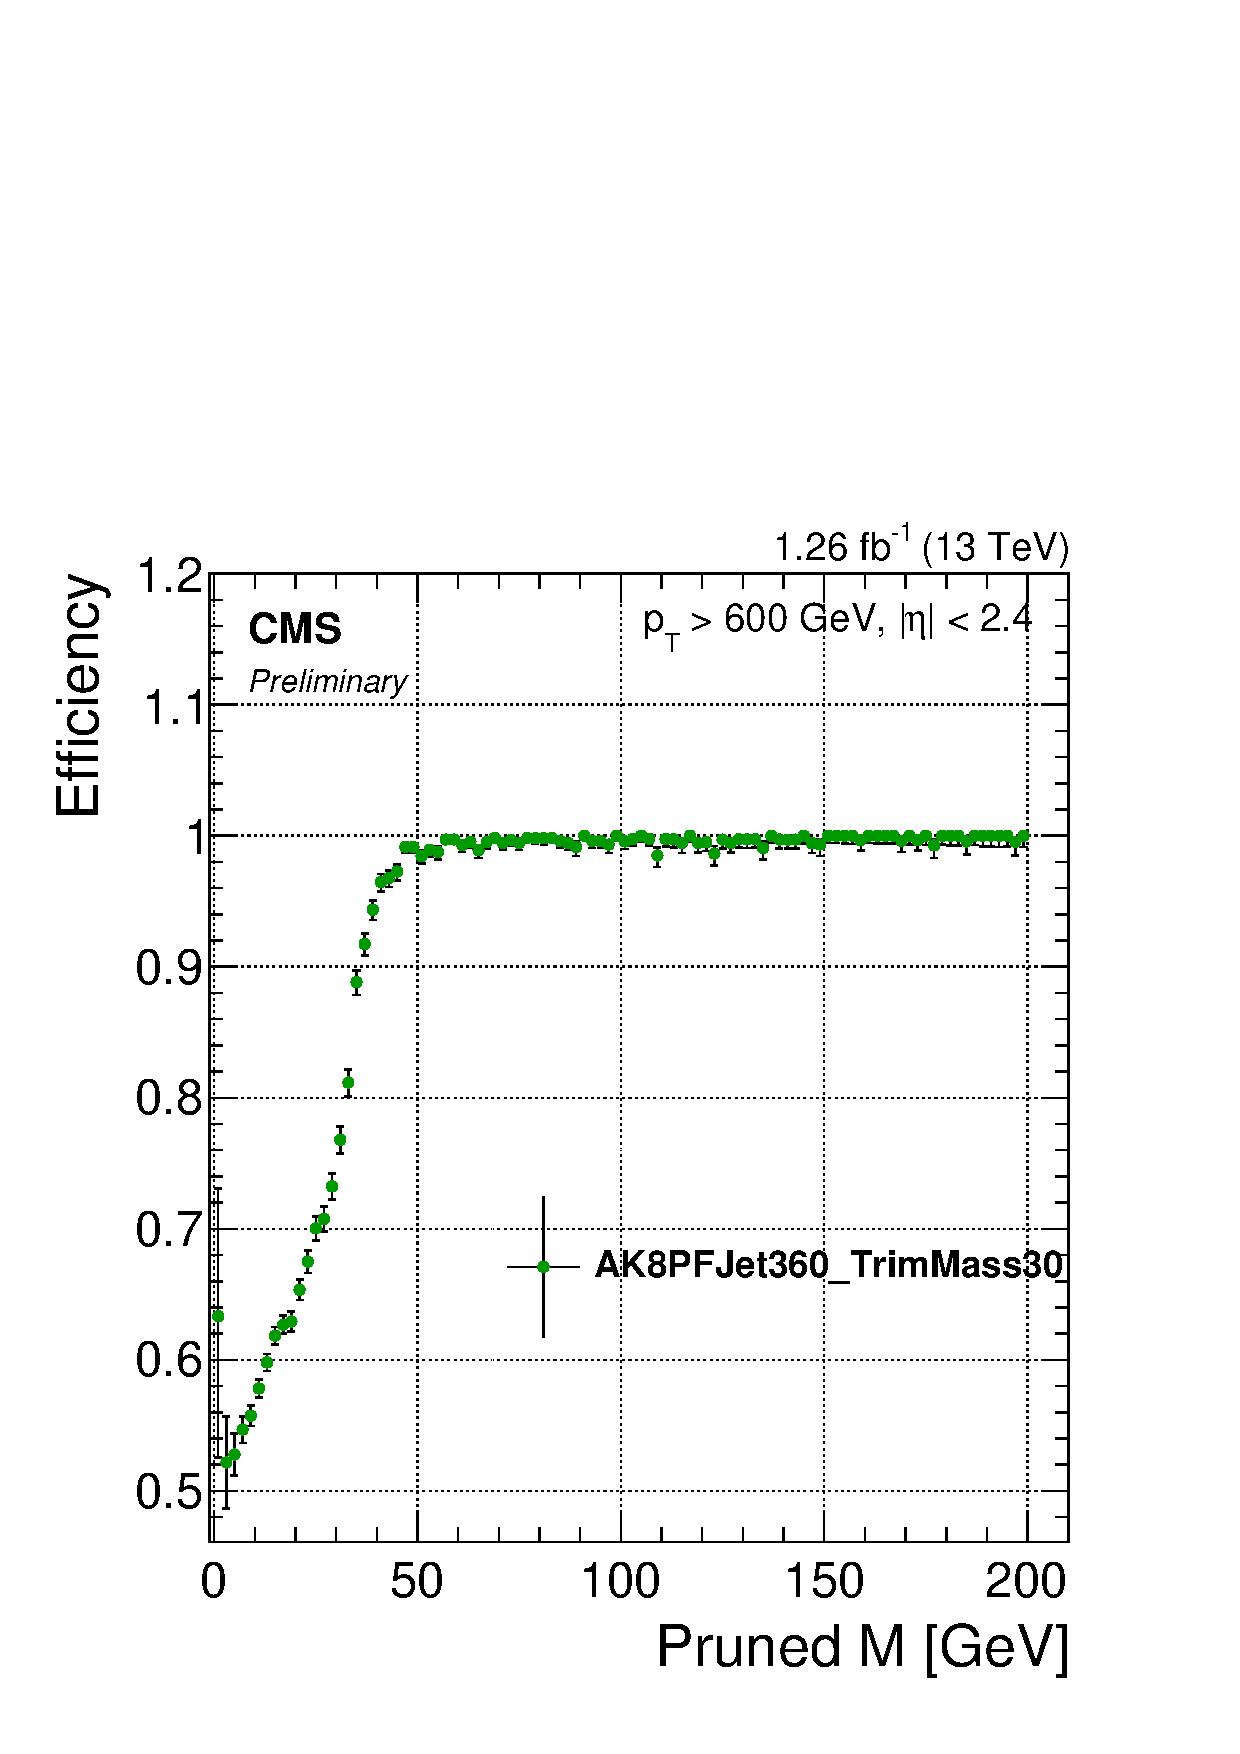
\includegraphics[width=0.4\textwidth]{figures/analysis/search1/AN-15-211//triggereff-prunedmass600.pdf}
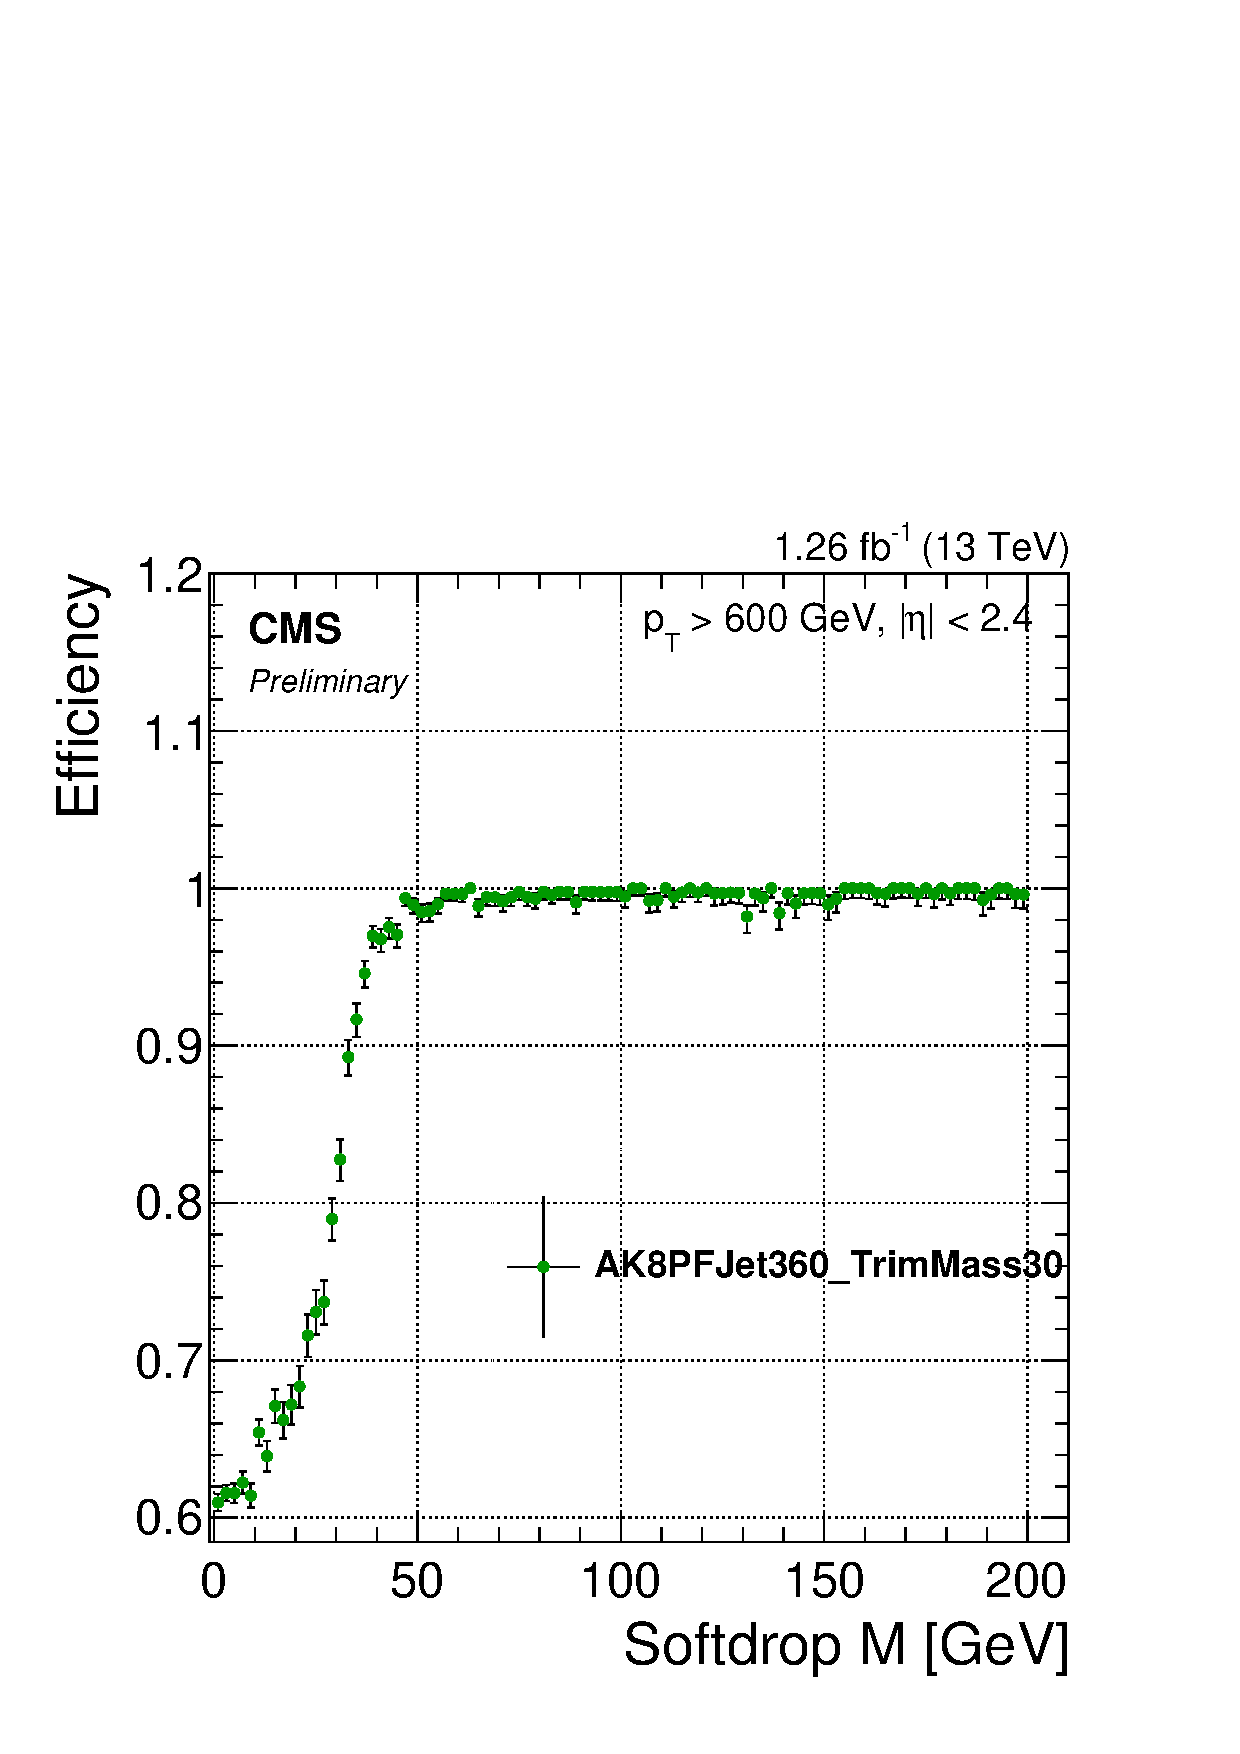
\includegraphics[width=0.4\textwidth]{figures/analysis/search1/AN-15-211//triggereff-sdmass.pdf}
\caption{Efficiency for the lowest threshold grooming trigger as a function of pruned-jet (left) and softdrop-jet (right) mass for jets with $\PT > \unit{600}{\GeV}$.}
\label{fig:searchI:grooming-mj-trigger}
\end{figure}


\subsubsection{Preselection} 
\label{sec:searchI:preselection}
After trigger selections and the corresponding requirement of a dijet invariant mass above 1 \TeV to ensure a smoothy falling background, the process of maximizing the signal significance while keeping the background low can begin. This is done through a set of jet requirements. The jets used in this analysis are clustered with the anti-\kt{} jet clustering algorithm with a clustering parameter of $R=0.8$ (see Section ~\ref{sec:objreco:jets}) to allow containment of the full vector boson decay products. These jets are further required to pass certain jet identification requirements provided by the JetMET POG~\cite{jetID_JME}, in order to distinguish them from fake jets. These are as follows:
\begin{itemize}
\item Number of Constituents $> 1$, for all jet $\eta$
\item Neutral Hadron Energy Fraction $< 0.90$, for all jet $\eta$
\item Neutral EM Energy Fraction $< 0.90$, for all jet $\eta$
\item Charged Hadron Multiplicity $> 0$, for jet $|\eta| < 3.0$
\item Charged EM Energy Fraction $< 0.99$, for jet $|\eta| < 3.0$
\end{itemize} 
Jets are further corrected for nonlinearities in $\PT$ and rapidity using standard jet energy corrections at CMS as described in Ref.~\cite{jme_jinst} for $R$=0.8 anti-\kt{} jets.
As we know that a minimum transverse of 200 \GeV is required for the decay products of a \PW/\PZ to be fully contained within an R=0.8 jet, events are further selected by requiring at least two jets with $\PT > \unit{200}{\GeV}$. These are in addition required to be central, with an $|\eta| < 2.4$. \par
The two highest \PT jets in the event passing these criteria are selected as potential vector boson candidates.
As our main background is QCD multijet events, we further take advantage of the fact that the angular distribution between these, mainly t-channel, processes are very different from the s-channel signal processes under study. The crossection for QCD t-channel processes as a function of the opening angle with respect to the beam axis ($\theta*$), exhibit a pole around $\cos \theta*=1$, meaning QCD t-channel jets are mostly forwardly produced, with an opening angle with respect to the beam axis close to zero. The signal jets on the other hand, produced through an s-channel process, are concentrated in the barrel region. We therefore require the jets to have a separation of $|\Delta\eta|<1.3$ in order to reduce the QCD multijets background.
The distribution of $|\Delta\eta|$ between the two highest-\PT jets for QCD as well as for different signal scenarios, is shown in Figure~\ref{fig:searchI:detaopt}

\begin{figure}[h!]
\centering
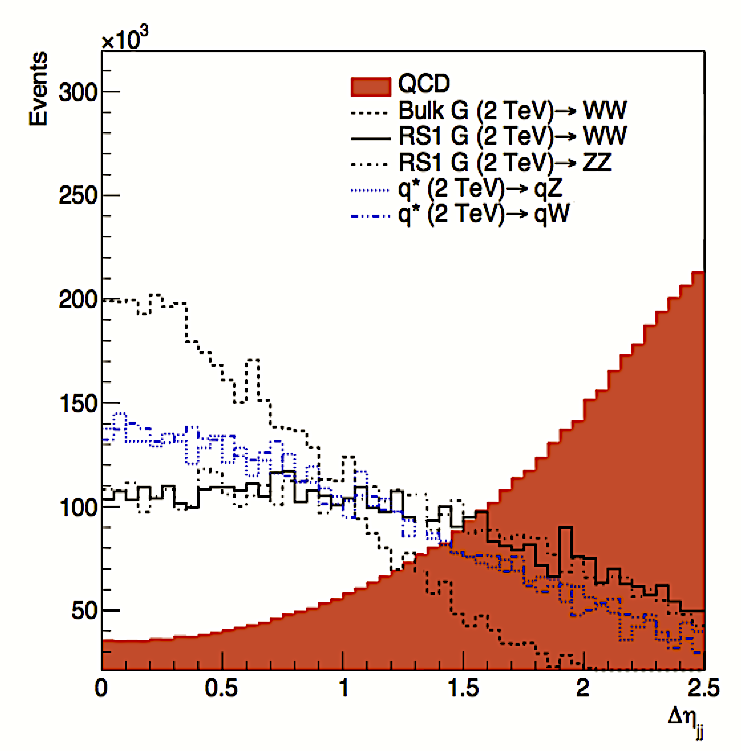
\includegraphics[width=0.4\textwidth]{figures/analysis/search1/misc/deta_opt.png}
\caption{ $|\Delta\eta|$  between the two highest-\PT jets for QCD jets and jets stemming from different signal scenarios.}
\label{fig:searchI:detaopt}
\end{figure}
 
A cut of $|\Delta \eta|_{jj}<1.3$ makes sure to remove the t-channel pole at $\cos \theta* = 1$ and is in addition found to yield the best separation between signal and the QCD background.
%
% A summary of the applied preselections is as follows:
%
% \begin{itemize}
% \item PF jet tight ID applied
% \item Jet $\eta < 2.4$
% \item Jet \pt $> 200$ GeV
% \item $|\Delta\eta|_{jj} < 1.3$
% \item Dijet invariant mass $> 1$ TeV
% \end{itemize}

The \PT, $\eta$, dijet invariant mass and $|\Delta \eta|_{jj}$ distribution for the two leading jets in the event after the above preselections have been applied is shown in Figure~\ref{fig:kinematics-all}.

\begin{figure}[h!]
\centering
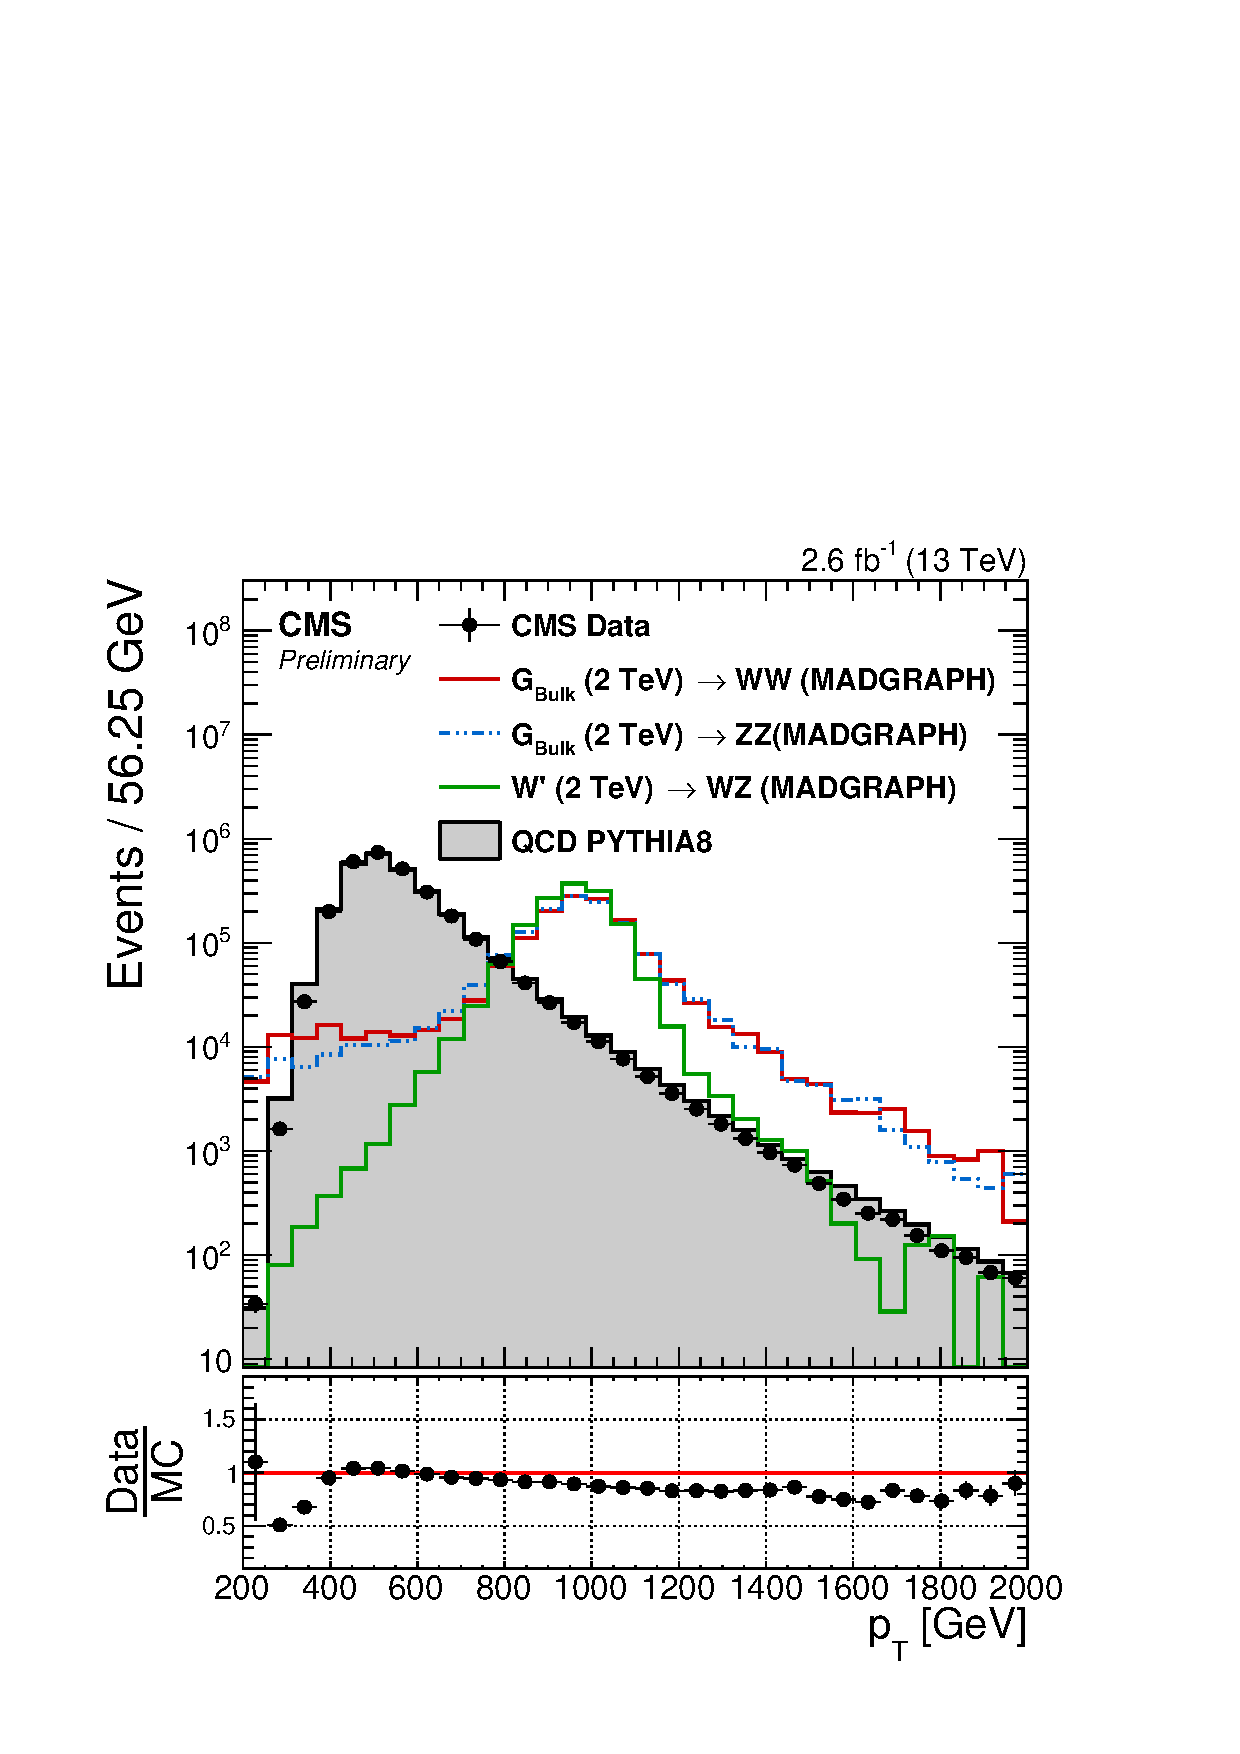
\includegraphics[width=0.4\textwidth]{figures/analysis/search1/AN-15-211/controlplots/silverjson/Pt_WSignal.pdf}
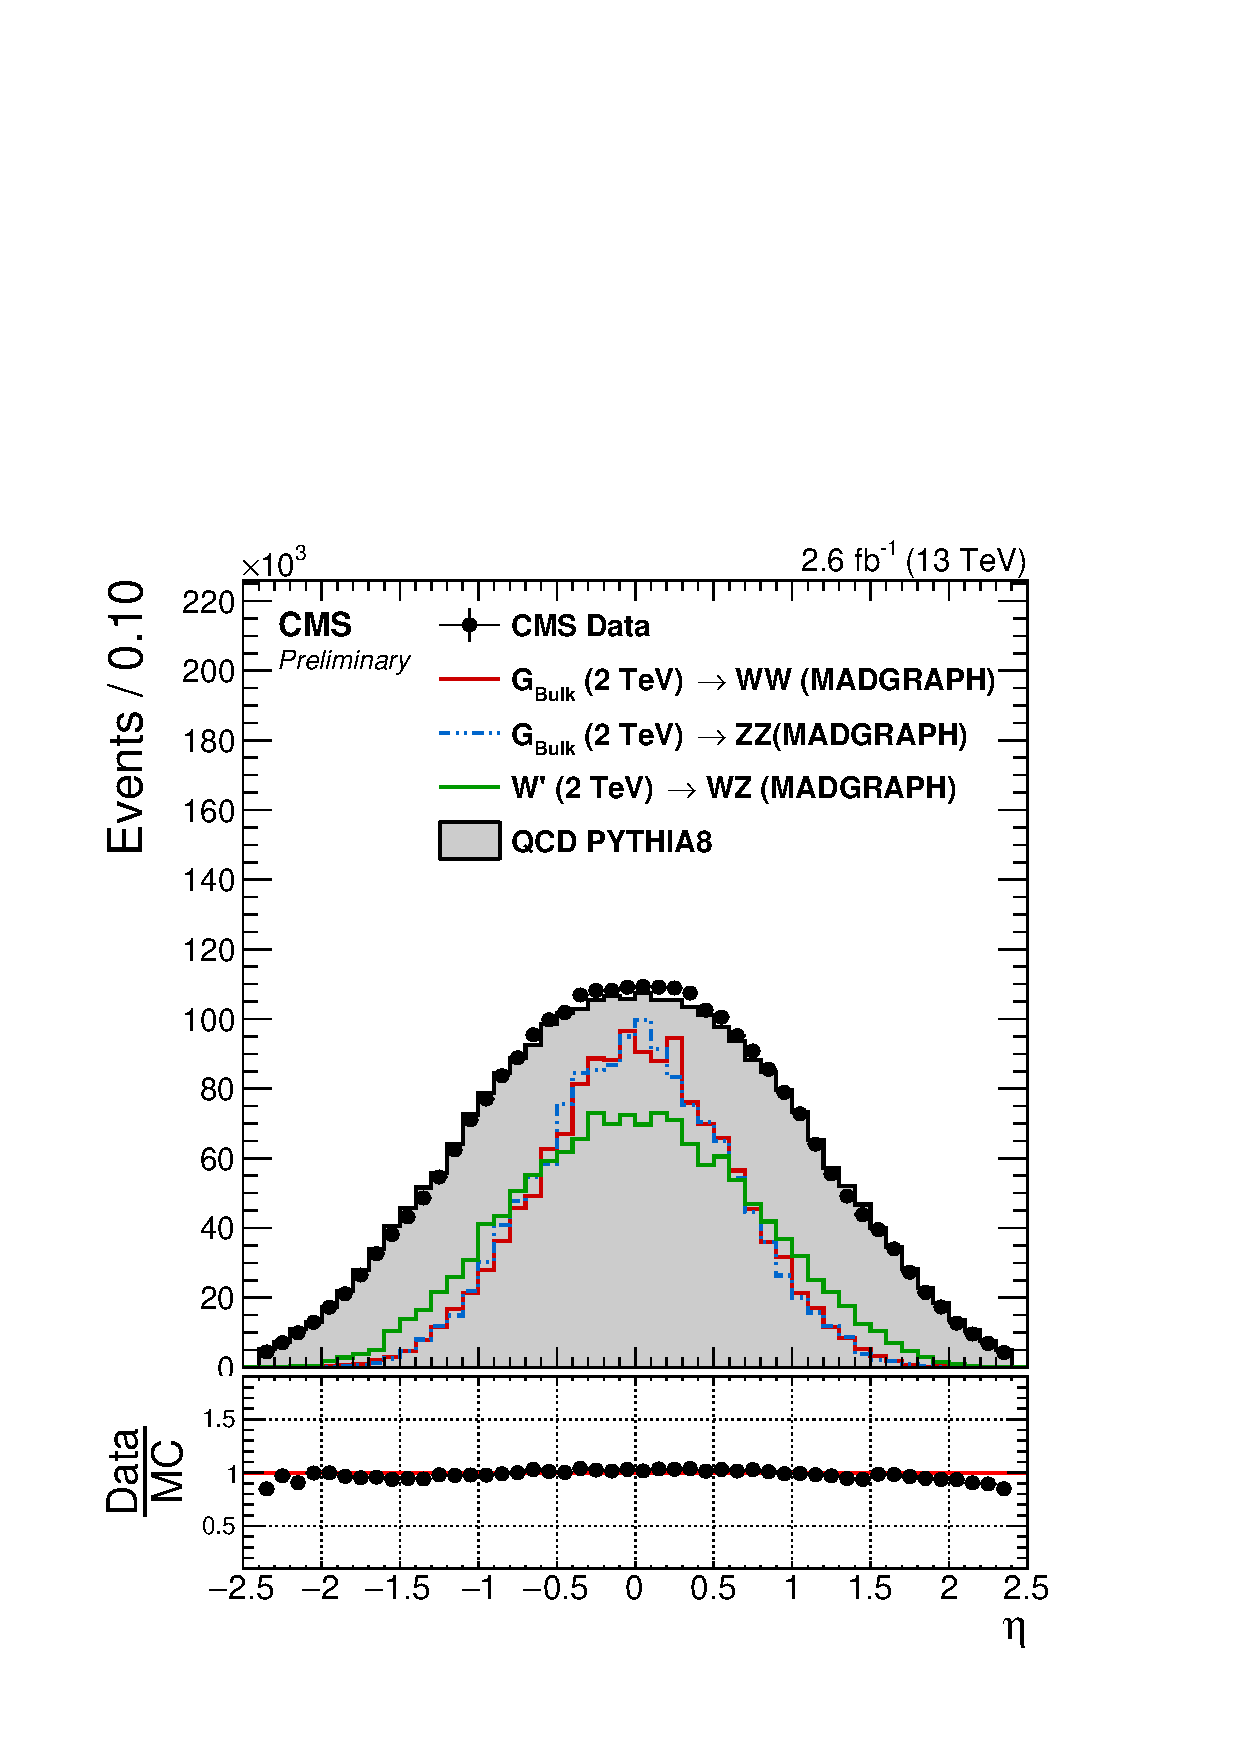
\includegraphics[width=0.4\textwidth]{figures/analysis/search1/AN-15-211/controlplots/silverjson/Eta_WSignal.pdf}\\
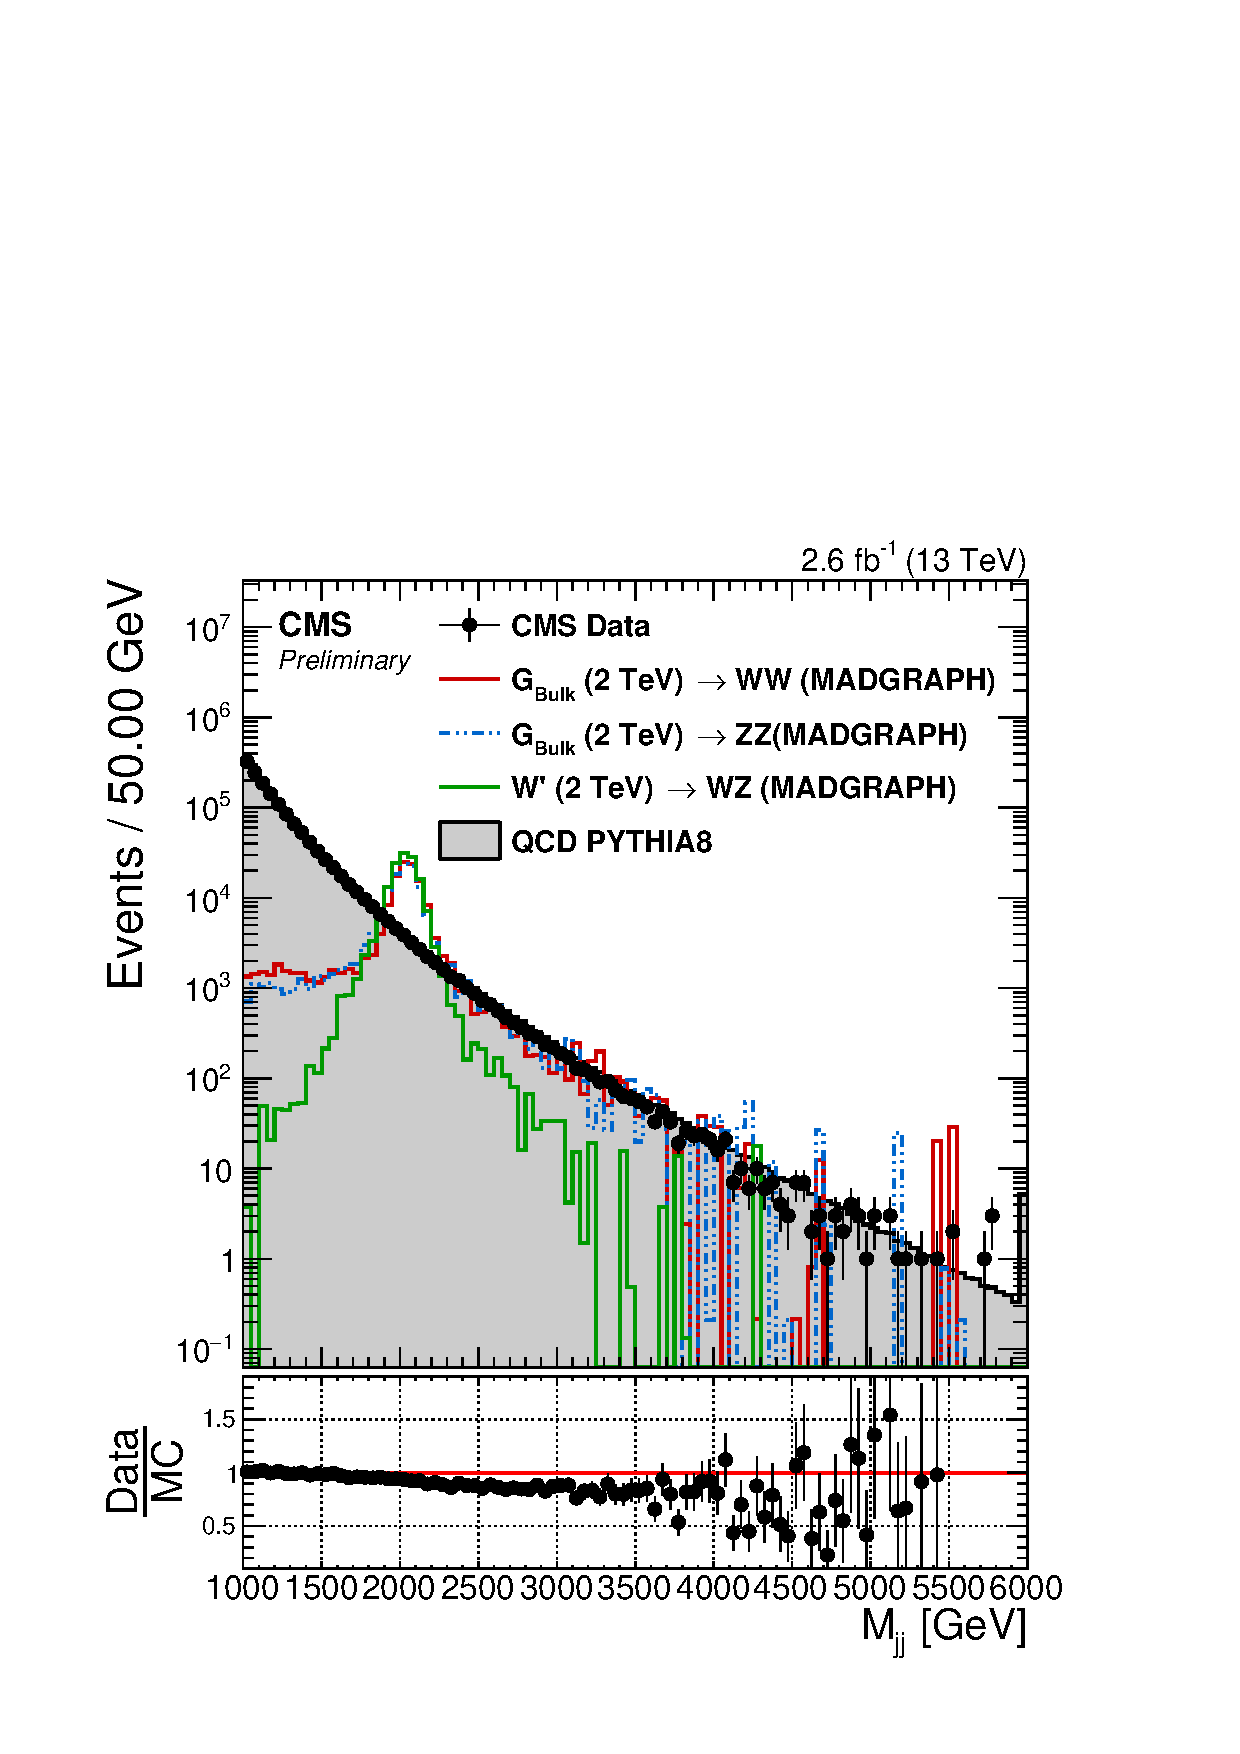
\includegraphics[width=0.4\textwidth]{figures/analysis/search1/AN-15-211/controlplots/silverjson/Mjj_WSignal.pdf}
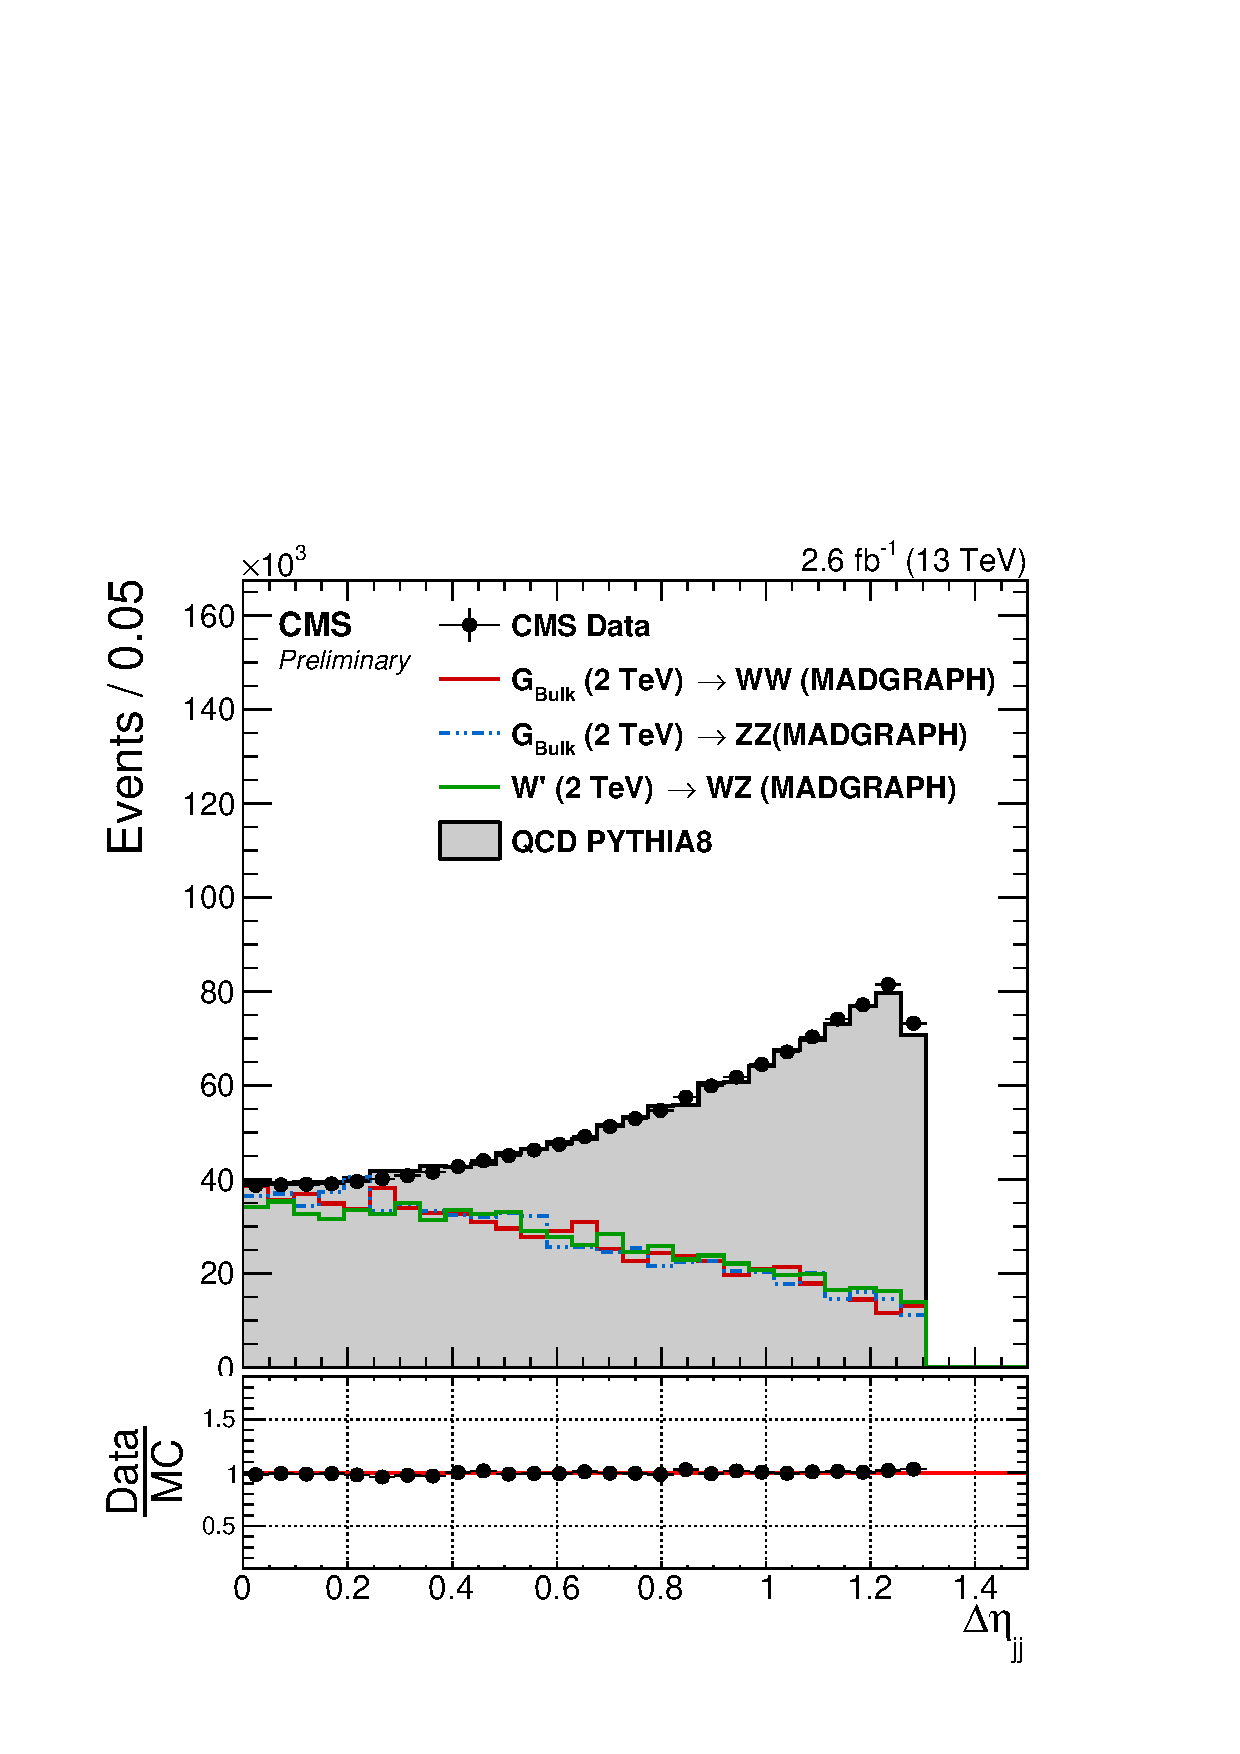
\includegraphics[width=0.4\textwidth]{figures/analysis/search1/AN-15-211/controlplots/silverjson/DeltaEta_WSignal.pdf}
\caption{Jet \PT (top left), $\eta$ (top right), dijet invariant mass (bottom left) and $|\Delta \eta|_{jj}$ (bottom right) distribution for the two leading jets in the event after loose preselections are applied. The signal is scaled by an arbitrary number.}
\label{fig:kinematics-all}
\end{figure}

\subsubsection{Vector boson tagging}
\label{sec:searchI:wtagging}
After preselections, we take advantage of the jet substructure algorithms described in Section~\ref{sec:objreco:substructure} to further separate boosted W/Z jets from the QCD multijets background. In the 8 \TeV analysis~\cite{Khachatryan:1700394} published the previous year, the pruning algorithm was the groomer of choice. However, recent progress had been made in the development of alternative groomers which had favorable properties from a theoretical point of view (see Sections~\ref{sec:objreco:grooming} and ~\ref{sec:searchII:puppisoftdrop}). We therefore studied two different grooming algorithms: pruning and softdrop (with $\beta=0$ and $z_{cut} = 0.1$). A comparison of the softdrop (dotted lines) and pruned (solid lines) jet mass for \PW, \PZ and \PH jets is shown in Figure~\ref{fig:searchI:sdvspruning}.

 \begin{figure}[h!]
 \centering
 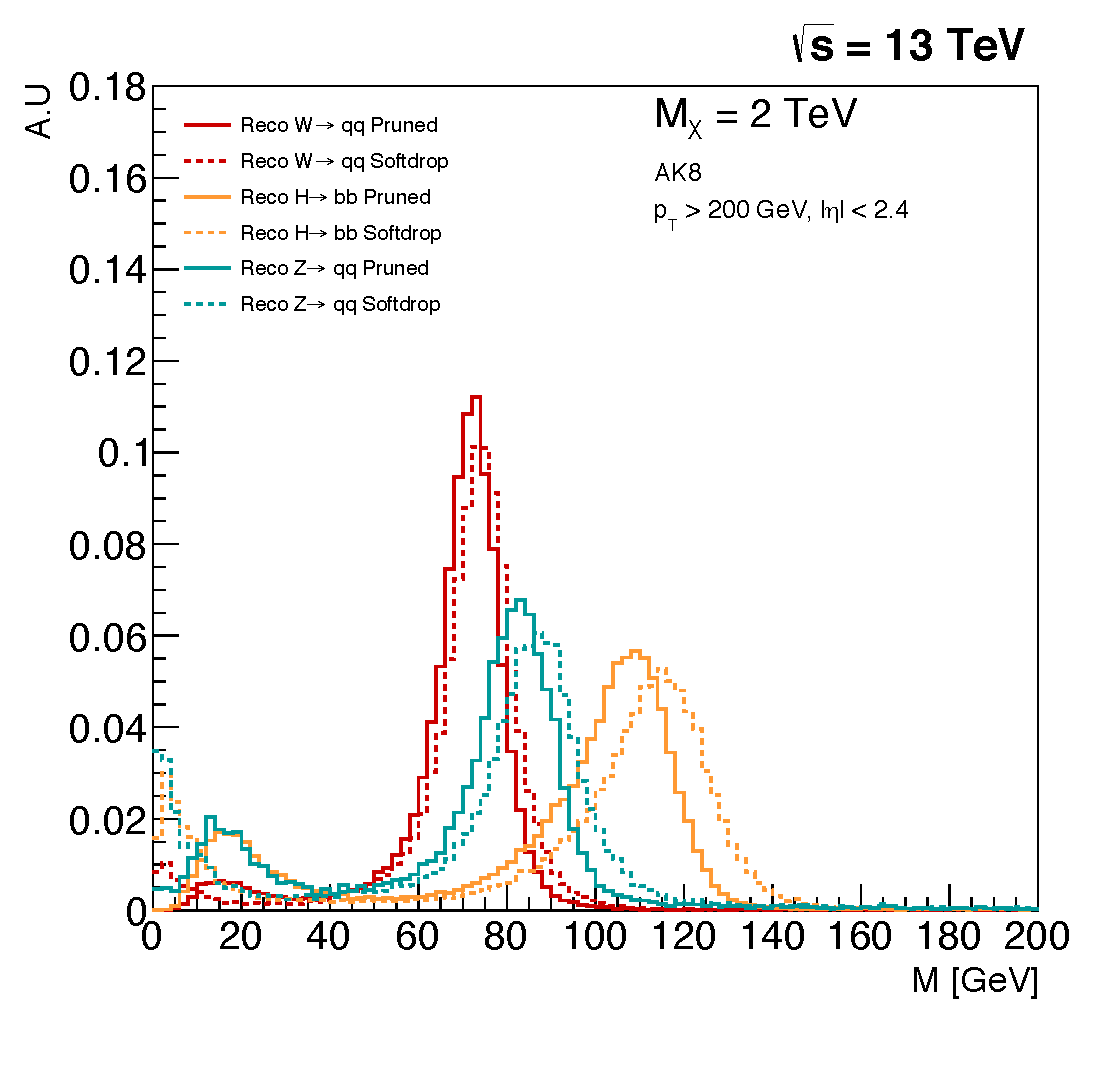
\includegraphics[width=0.49\textwidth]{figures/analysis/search1/misc/SDvsPruned.pdf}
 \caption{The softdrop (dotted lines) and the pruned (solid lines) jet mass for \PW, \PZ and \PH jets.}
 \label{fig:searchI:sdvspruning}
 \end{figure}
 
One of the first observations we made comparing the two groomers, was that there appeared to be a strong dependence of softdrop mass on the jet \PT. Figure~\ref{fig:searchI:grommedmassshift} shows the pruned (left) and softdrop (right) mass distributions for \PW jets coming from the decay of a \BulkG with a resonance mass of $0.8 \TeV < \mX < 4 \TeV$. While the pruned jet mass mean appeared stable as the jet transverse momenta of the jet increased ($\PT\sim\mX/2$), the softdrop jet mass mean shifted towards lower values as jet \PT increased.



\begin{figure}[h!]
\centering
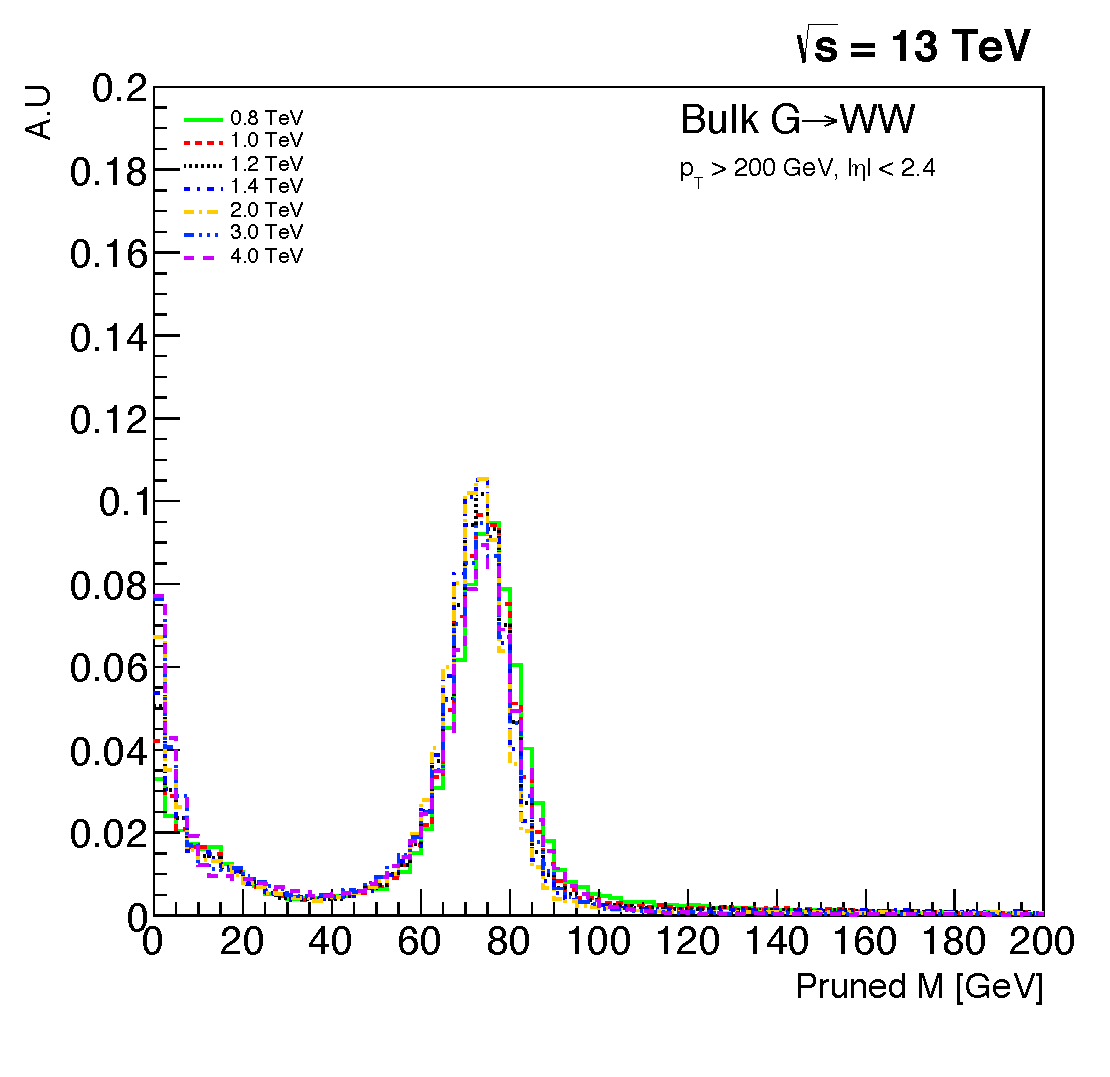
\includegraphics[width=0.49\textwidth]{figures/analysis/search1/misc/pruned_mass_shift.pdf}
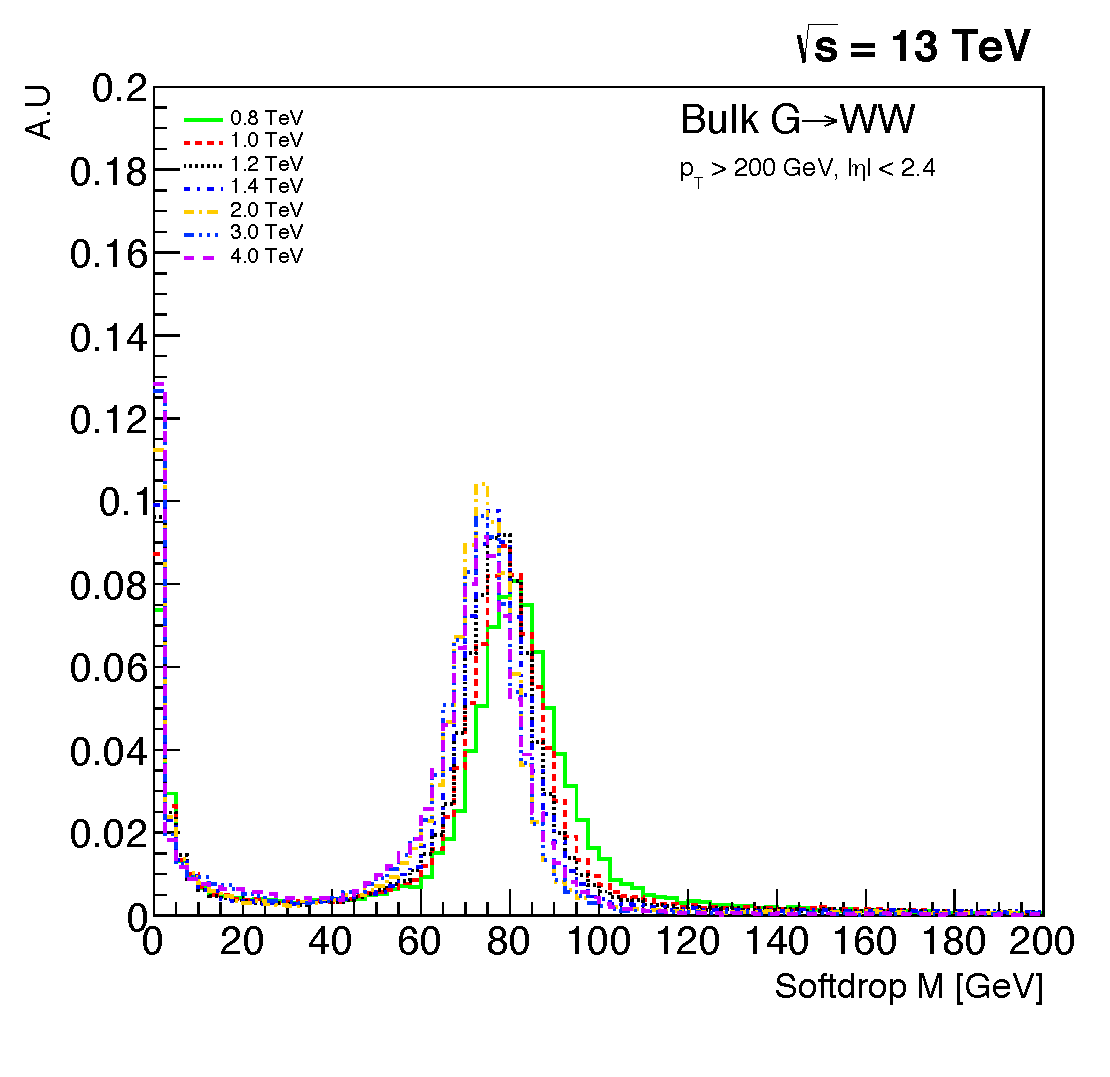
\includegraphics[width=0.49\textwidth]{figures/analysis/search1/misc/softdrop_mass_shift.pdf}
\caption{The jet mass distribution for W jets coming from a $\textrm{G}_{\textrm{bulk}}$ of masses in the range $0.8 \TeV < \mX < 4 \TeV$ decaying to \WW, here with pruning applied (left) and softdrop (right). A strong shift in the jet mass mean as a function of \PT ($\sim\mX/2$), is observed for jets groomed with the softdrop algorithm. Charge hadron subtraction is applied to all jets before clustering.}
\label{fig:searchI:grommedmassshift}
\end{figure}

In order to investigate whether this was a reconstruction effect or an algorithmic effect, we additionally looked at the pruned and softdrop mass for generator level jets (jets clustered with generator level particles before they are passed through the detector simulation). Figure~\ref{fig:searchI:grommedmassshift_genvsreco} shows the reconstructed (solid line) and generator level (dotted line) jet mass distributions after pruning (left) or softdrop (right) have been applied. Again, the distributions are compared for jets with very different \PT profiles, here for W jets coming from a $\BulkG \rightarrow \WW$ of mass $\mX = 0.8 \TeV$ (red), roughly $\PT\sim 400 \GeV$, and $\mX = 2.0 \TeV$ (blue), $\PT\sim 1 \TeV$.
Interestingly, we observe a \PT-dependent mass shift already for generator level softdrop jets (comparing the dotted lines in the right plot); an effect further enhanced at reconstruction level. This effect is not present for pruned jets, neither at generator level nor reconstruction level.


\begin{figure}[h!]
\centering
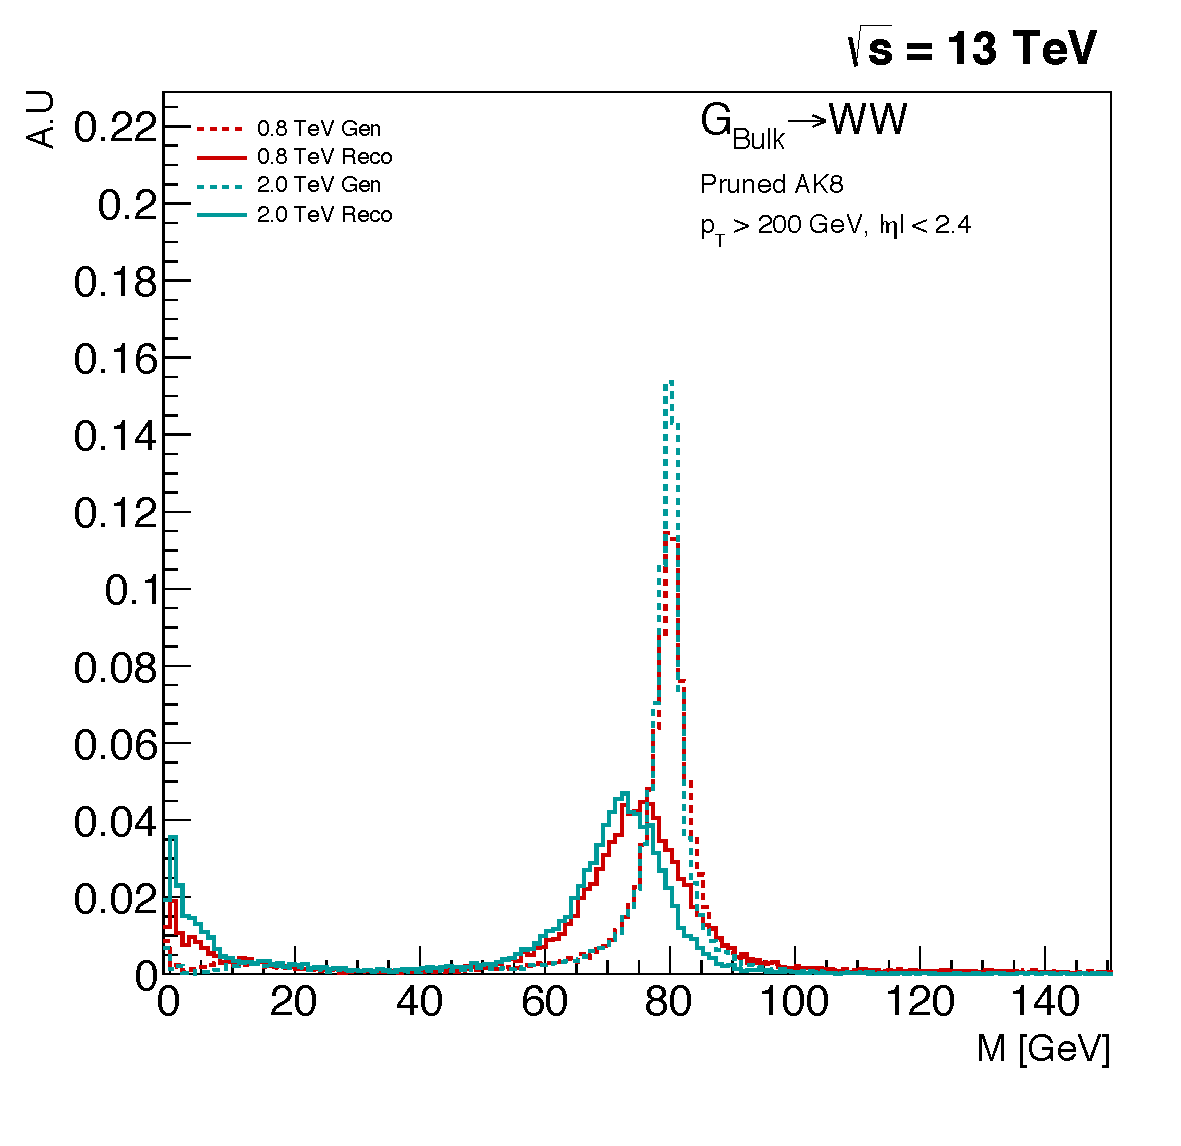
\includegraphics[width=0.49\textwidth]{figures/analysis/search1/misc/pruned_mass_shift_genvsreco.pdf}
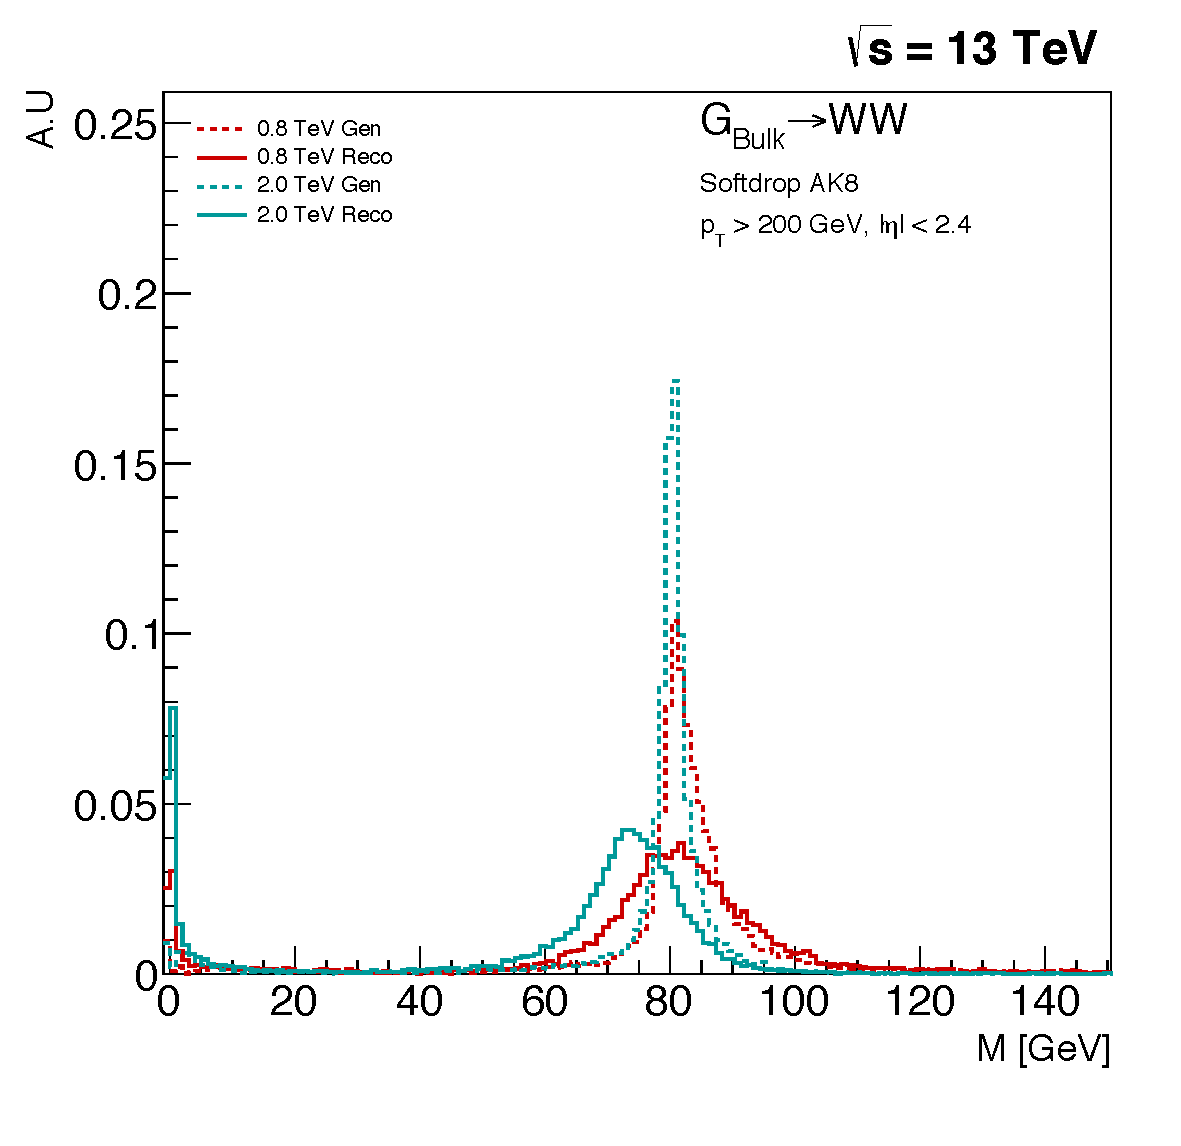
\includegraphics[width=0.49\textwidth]{figures/analysis/search1/misc/softdrop_mass_shift_genvsreco.pdf}
\caption{The reconstructed (solid line) and generator level (dotted line) jet mass distribution for W jets coming from a $\BulkG \rightarrow \WW$ of mass $\mX = 0.8 \TeV$ (red), roughly $\PT\sim 400 \GeV$, and $\mX = 2.0 \TeV$ (blue), $\PT\sim 1 \TeV$. Here for the pruned (left) and softdrop (right) jet mass.}
\label{fig:searchI:grommedmassshift_genvsreco}
\end{figure}

The observed softdrop mass \PT-dependence was problematic, due to the fact that it would require a \PT dependent mass window. This would again require several different measurements of data to simulation tagging efficiency scale factors, for the respective mass windows, or a significantly higher uncertainty on the signal yield. Due to these observations, the grooming algorithm of choice for this analysis is pruning, with $65 \GeV < m_{pruned} < 105 \GeV$. However, this would be a study we would return to in Search II (Section~\ref{searchII}).
\newline\newline
The shape tagger we chose for this analysis was the n-subjettiness ratio \nsubj. \nsubj is strongly correlated to the pruned jet mass, and the discriminating power of the variable is reduced when applying a pruned mass cut. The \nsubj distribution for the QCD background and \PW jets from a signal decay before (left) and after (right) a pruned mass cut of $65 \GeV < m_{pruned} < 105 \GeV$ have been applied, is shown in Figure~\ref{fig:searchI:tau21_groomedvsungroomed}.

\begin{figure}[h!]
\centering
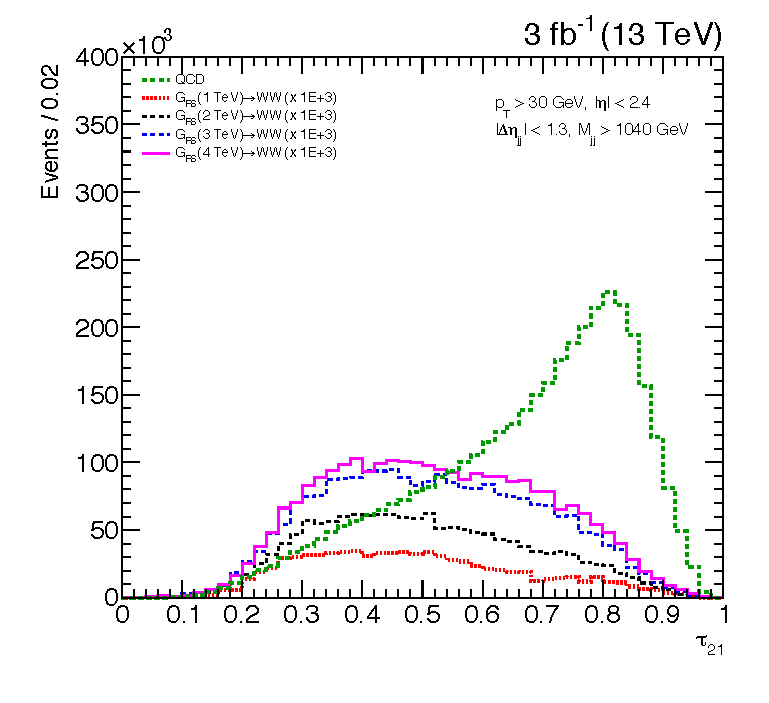
\includegraphics[width=0.49\textwidth]{figures/analysis/search1/misc/tau21_ungroomed.pdf}
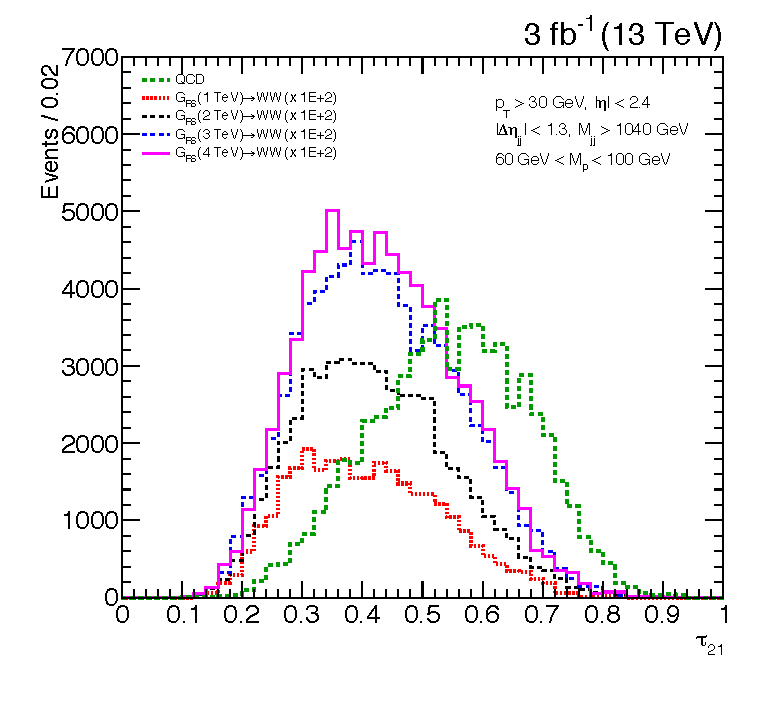
\includegraphics[width=0.49\textwidth]{figures/analysis/search1/misc/tau21_groomed.pdf}
\caption{The \nsubj distribution for QCD background and signal jets before (left) and after (right) a pruned mass window is applied. The discriminating power of \nsubj is strongly reduced after grooming.}
\label{fig:searchI:tau21_groomedvsungroomed}
\end{figure}

We therefore perform a cut optimization on \nsubj after all analysis selections, including a pruned mass window of $65 \GeV < m_{pruned} < 105 \GeV$, have been applied. This is done by scanning the \nsubj cut, and for each cut computing the Punzi significance~\cite{Punzi:2003bu} defined as
\begin{equation*}
\textrm{S} = \frac{\epsilon_S}{1+\sqrt{\textrm{B}}}  
\end{equation*}  
where $\epsilon_S$ is the signal efficiency and B is the total background. The cut with the highest significance is defined as the optimal cut value. The signals under consideration are W jets coming from the decay of a \BulkG with $\mX = 1-4 \TeV$, against a background of light flavored QCD jets. Only jets with a dijet invariant mass in a 20\% window around the resonance mass are considered. The Punzi significance as a function of the upper cut value on \nsubj is shown on the left in Figure~\ref{fig:searchI:tau21_punzi}.

\begin{figure}[h!]
\begin{center}
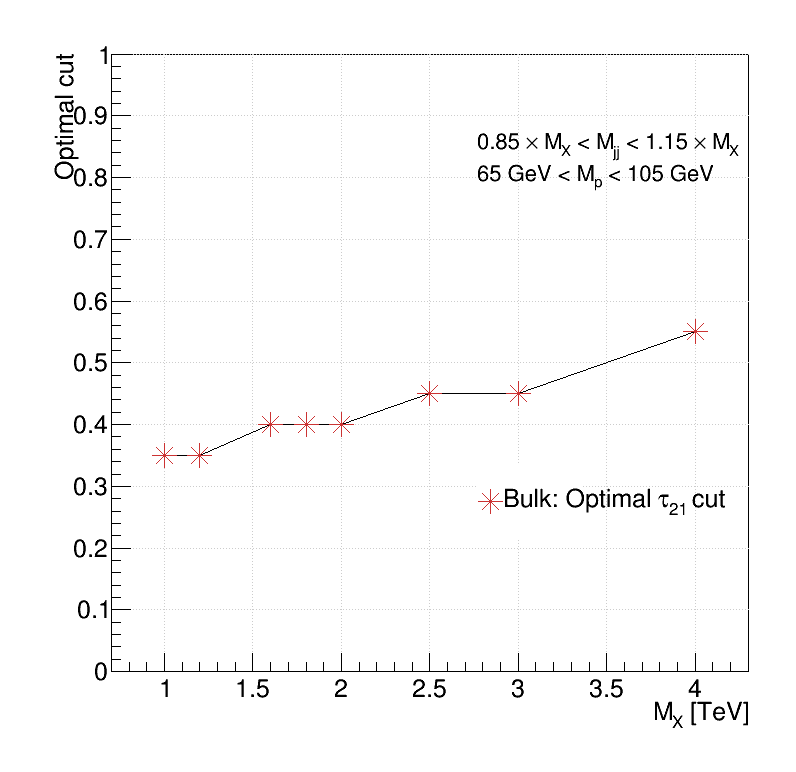
\includegraphics[width=0.49\textwidth]{figures/analysis/search1/AN-15-196/tau21optimisation/HP_Punzi_BulkWW.png}
%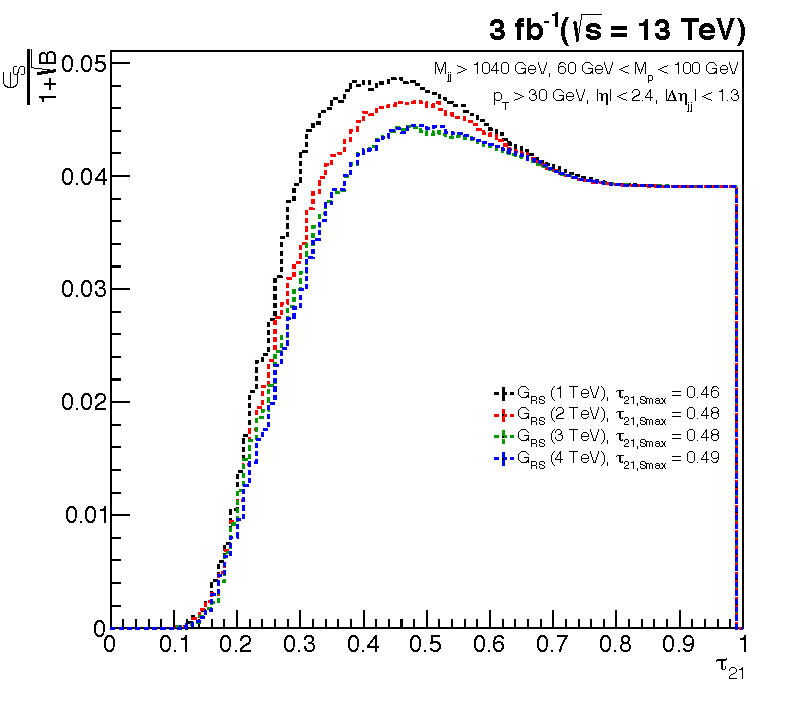
\includegraphics[width=0.49\textwidth]{figures/analysis/search1/misc/tau21_punzi.pdf}
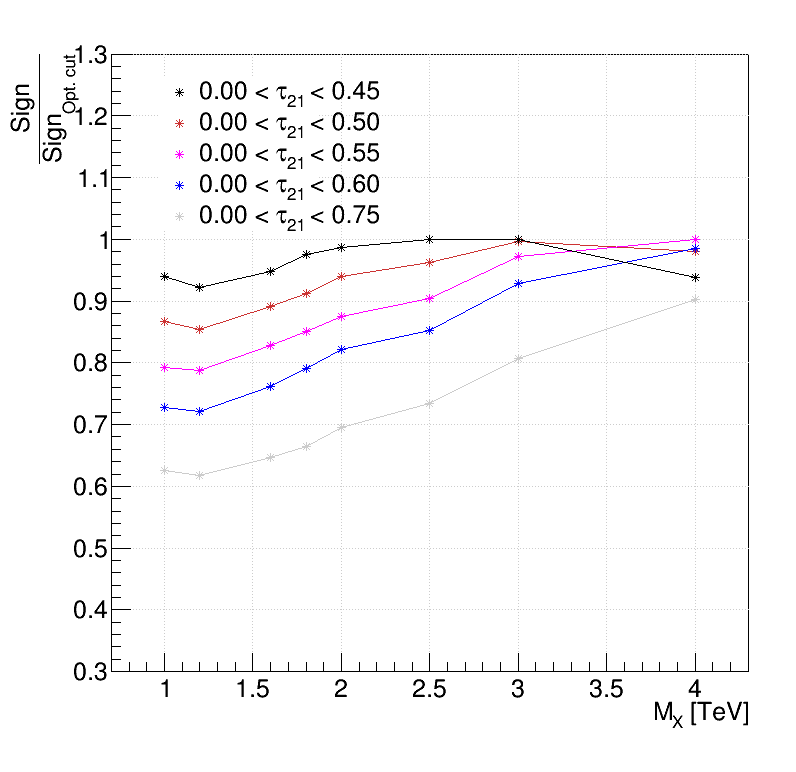
\includegraphics[width=0.49\textwidth]{figures/analysis/search1/AN-15-196/tau21optimisation/HP_CutSignificance_bulkWW.png}\\
\caption{Optimal upper cut on $\tau_{21}$ as a function of \BulkG mass (left).  The optimal $\tau_{21}$ selection for W' (HTV model) resembles the Bulk graviton selection.}
\label{fig:searchI:tau21_punzi}
\end{center}
\end{figure}

The optimal cut gets looser as the dijet invariant mass increases, something which can be understood when looking at the QCD dijet invariant mass spectrum in Figure~\ref{fig:kinematics-all}. The number of QCD jets falls of exponentially with \mjj, meaning that the background at 4 \TeV is considerably lower than at 1 \TeV. This allows for a looser cut on \nsubj as \mjj increases. In order to choose a single cut which works reasonably well for all masspoints, we look at the ratio of a given \nsubj cut over the significance of the best cut at that mass points. This is shown in the right plot of Figure~\ref{fig:searchI:tau21_punzi}. The cut $\tau_{21}<0.45$ has the most stable performance out of the investigated cut values and is due to that, and due to the desire of keeping the background as low as possible at low \mjj, chosen as the nominal cut. In order to account for the fact that background is lower at high-\mjj, we add an additional analysis category, $0.45 < \nsubj < 0.75$, which contains $>95\%$ of the signal and enhances the analysis sensitivity where the background is low.
These categories are hereafter referred to as the "high purity" (HP) category, for jets with $0<\tau_{21} \leq 0.45$, and the low purity (LP) caegory, for jets with $0.45<\tau_{21}\leq0.75$.
\newline
\newline
The W-tagging efficiency and QCD light-flavored jet mistagging rate for a W-tagger consisting of $0<\tau_{21} \leq 0.45$ and  $65 \GeV < m_{pruned} < 105 \GeV$ is shown in Figure~\ref{fig:searchI:wtageff}, both as a function of jet \PT and as a function of number of primary vertices in the event.


\begin{figure}[h]
\begin{center}
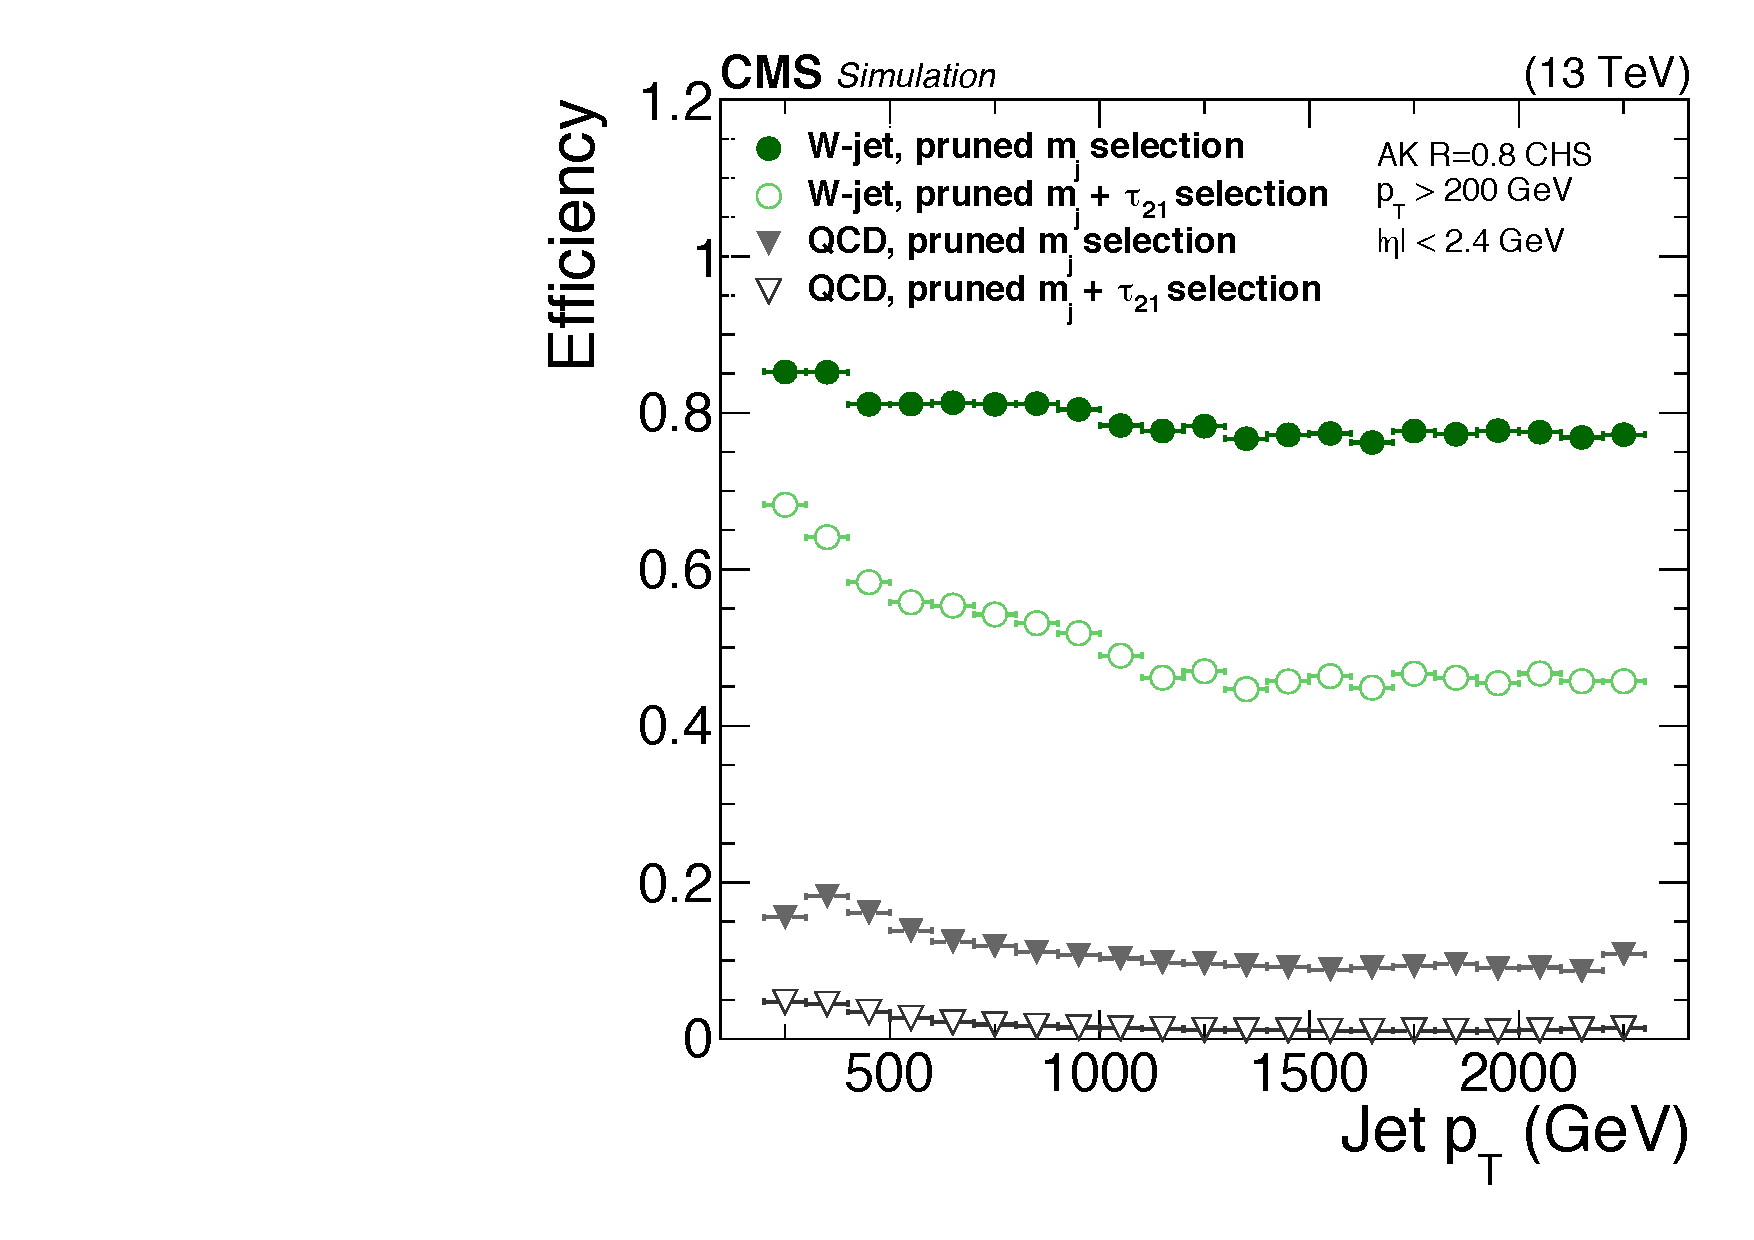
\includegraphics[width=0.49\textwidth]{figures/analysis/search1/misc/WtagSigEff_vpT_pruned.pdf}
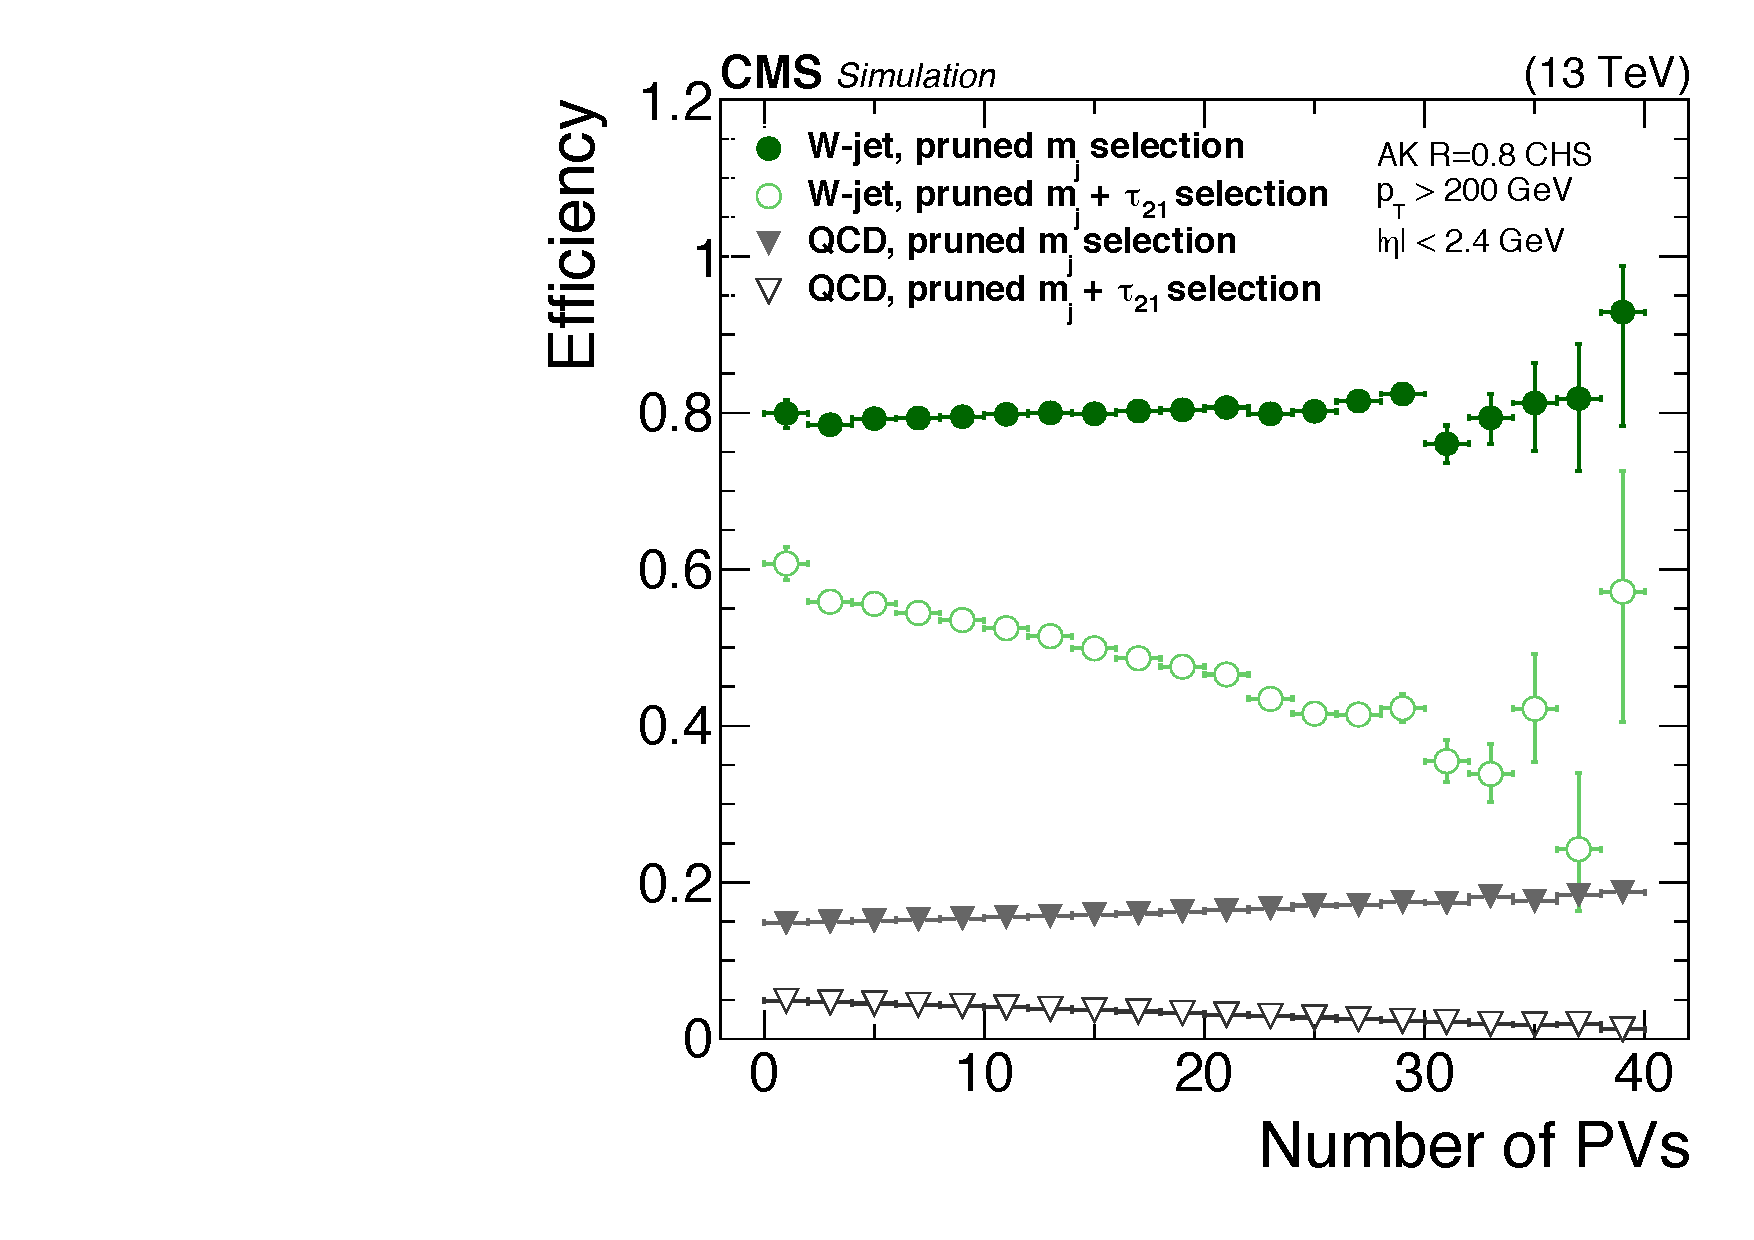
\includegraphics[width=0.49\textwidth]{figures/analysis/search1/misc/WtagSigEff_vnPVs_pruned.pdf}
\caption{The W-tagging efficiency (green) and light jet mistag rate (grey) for a pruned jet mass cut only and pruned jet mass + \nsubj cut as a function of \PT (left) and number of primary vertices (right). }
\label{fig:searchI:wtageff}
\end{center}
\end{figure}


The signal efficiency for a pruned jet mass cut only, is around 80 \% with a mistag rate of $\sim 15\%$. After adding a \nsubj cut, the signal efficiency drops to around 55\% and the mistagging rate to $\sim 2\%$. Another interesting feature is the dependence of \nsubj on \PT on pileup, compared to the resilience of the groomed mass as a function of the same variables. This will be another feature we explore in Search II (Section~\ref{searchII}).






Figure~\ref{fig:wtag} shows the pruned-jet mass (left) and the n-subjettiness $\tau_{21}$ distribution (right) for signal and background Monte Carlo, as well as the distributions measured in data. 

\begin{figure}[h!]
\centering
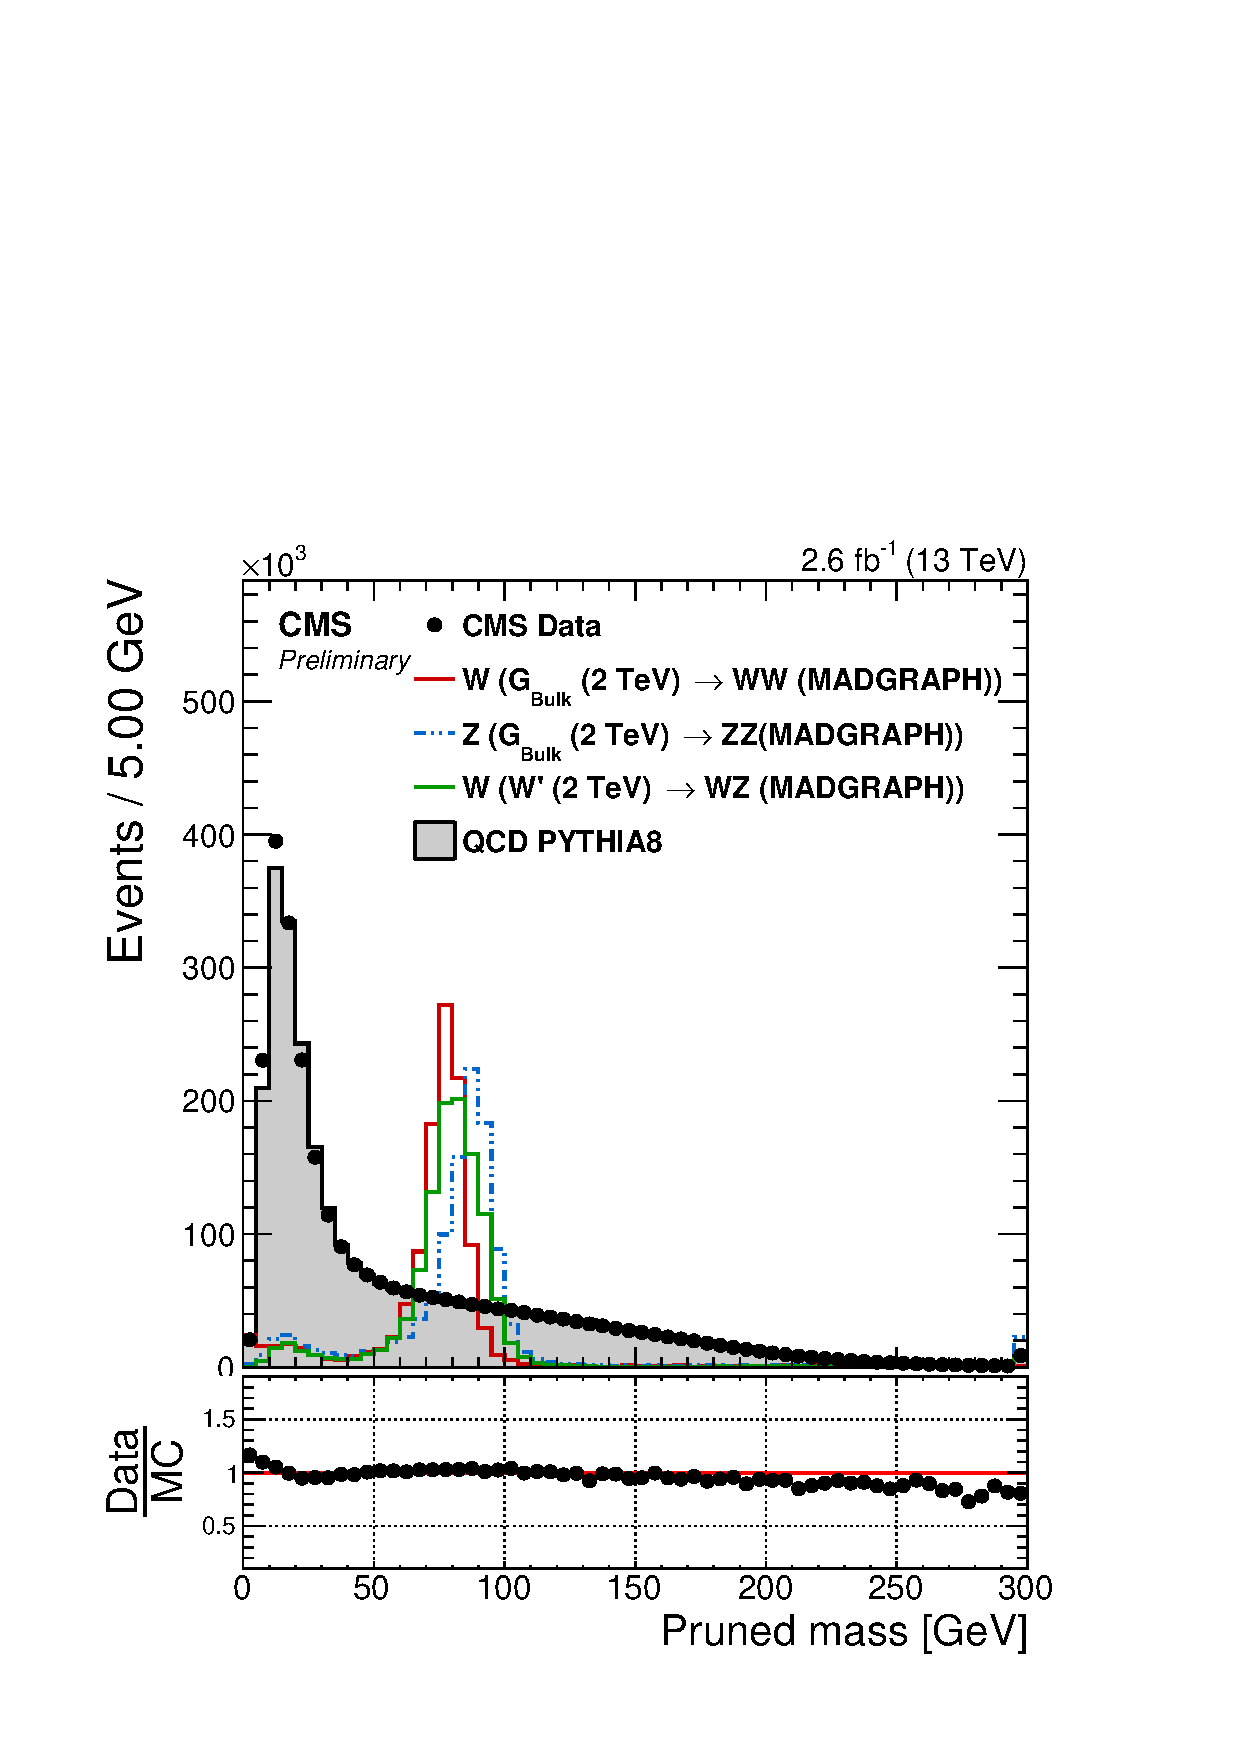
\includegraphics[width=0.4\textwidth]{figures/analysis/search1/AN-15-211/controlplots/silverjson/PrunedMass_WSignal.pdf}
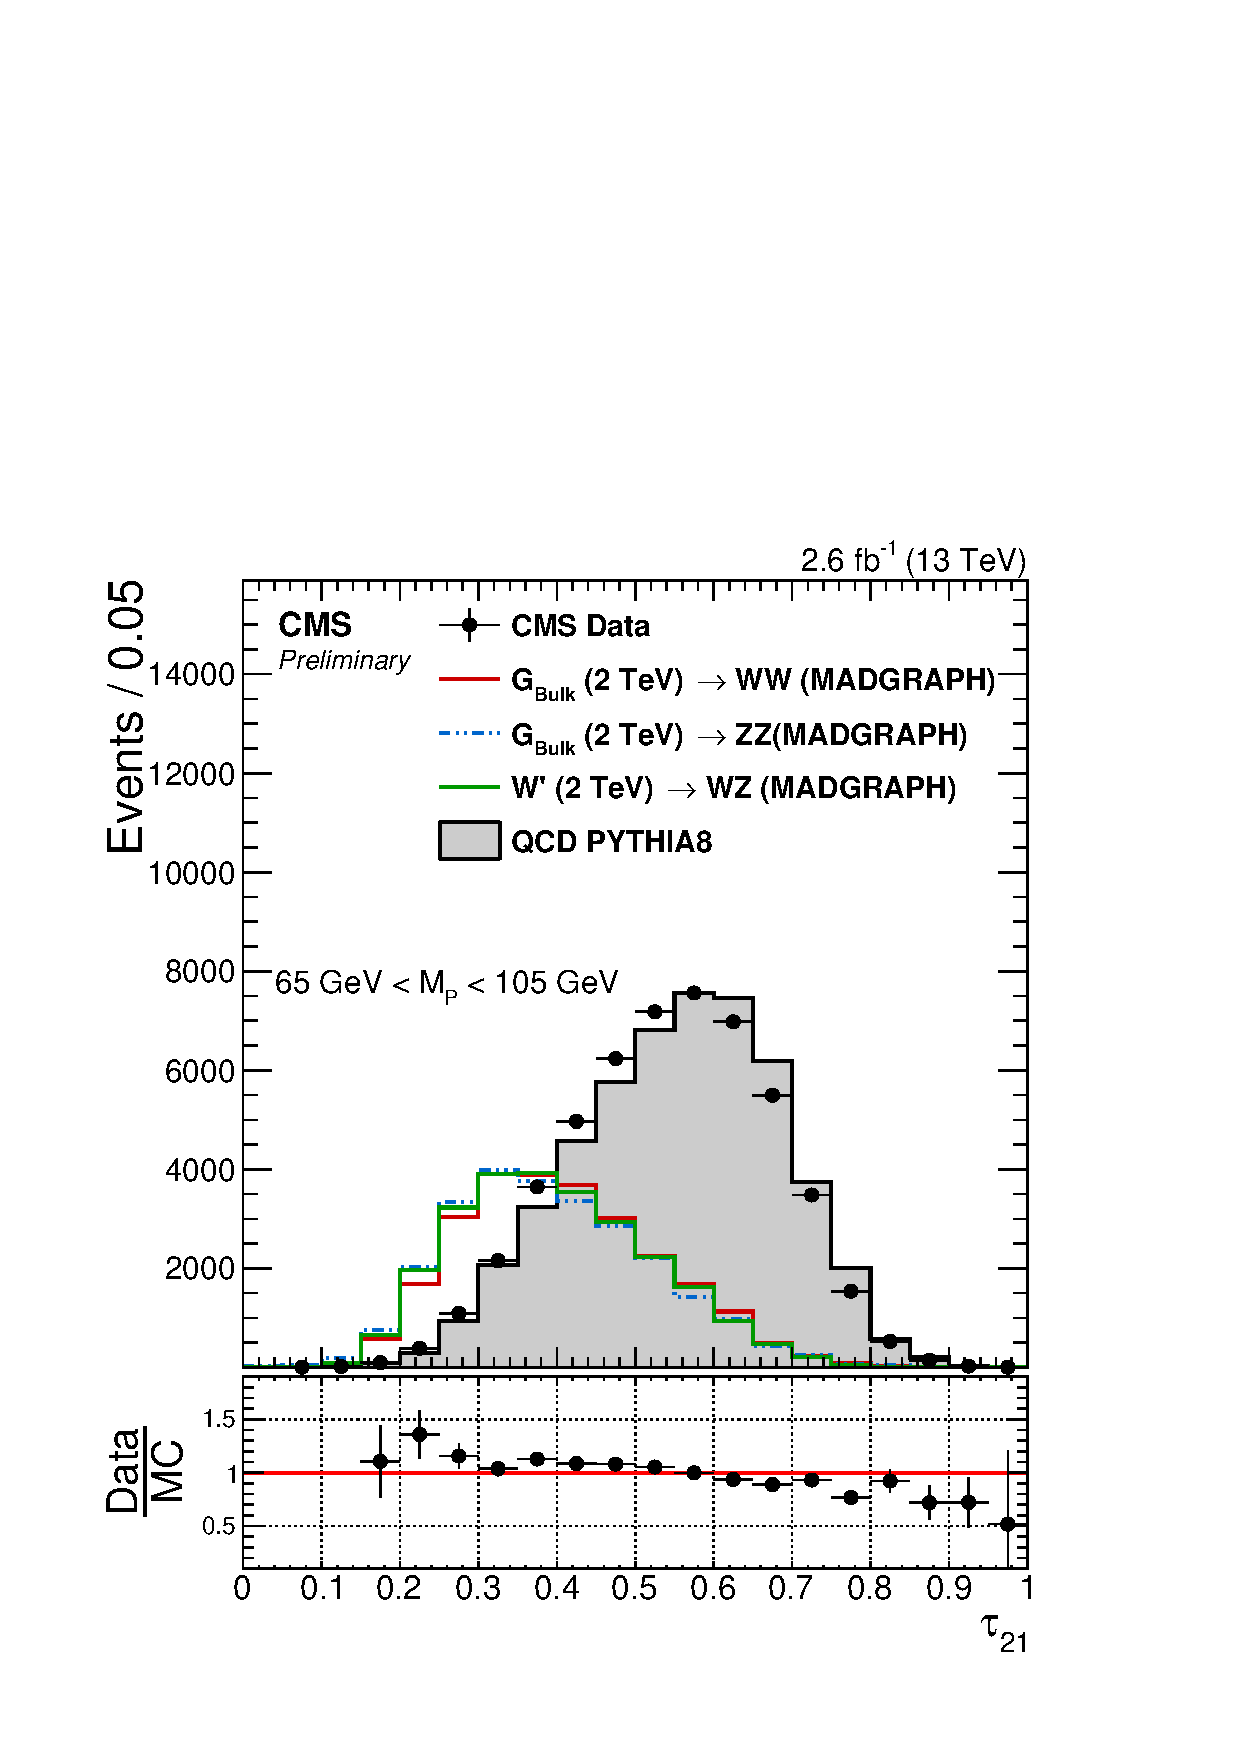
\includegraphics[width=0.4\textwidth]{figures/analysis/search1/AN-15-211/controlplots/silverjson/Tau21_punzi_WSignal.pdf}\\
\caption{Pruned jet mass distribution (left) and n-subjettiness $\tau_{21}$ (right) distribution for data and simulated samples. Simulated samples are scaled to match the distribution in data. The $\tau_{21}$ distribution is shown for jets after a cut of $65 {\GeV} < M_{p} < 105 {\GeV}$ has been applied.}
\label{fig:wtag}
\end{figure}


\subsubsection{Analysis categorization}
As the analysis requires two W/Z-tags, we always require one HP tagged jet and then divide into LP and HP categories depending on whether the other jet is of high or low purity. In addition, in order to further enhance the analysis sensitivity, we further split the pruned jet mass window into a W and a Z boson window where the W window is defined as $65 {\GeV} < m_{pruned} < 85 {\GeV}$ and the Z boson window as $85 {\GeV} < m_{pruned} < 105 {\GeV}$. This has the added benefit of allowing us to make a discrimination between a \BulkG decaying to \WW or \ZZ, and a \PWpr decaying into \WZ through counting events in each category. We, for instance, expect a higher signal yield in \WZ category for a \PWpr decaying to a \PW and \PZ boson then for a \BulkG decaying to \WW or \ZZ. Figure~\ref{fig:searchI:massCatWpr} shows the relative expected signal yield (left) and expected limits (left) in the different mass categories for a 2 \TeV \PWpr.
 
 \begin{figure}
 \centering
 \begin{minipage}{0.5\textwidth}
 \centering
 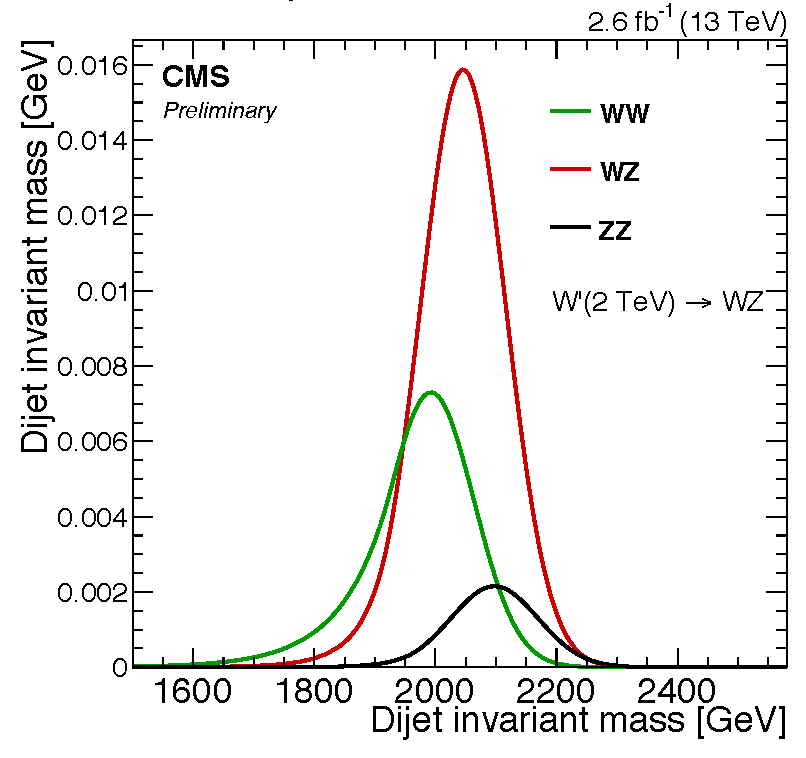
\includegraphics[width=0.99\textwidth]{figures/analysis/search1/misc/massCategories.pdf}
 \end{minipage}
 \begin{minipage}{0.29\textwidth}
 \centering
 \captionsetup{type=table} %% tell latex to change to table
 \begin{tabular}{| l | c |}
 \hline
 \multicolumn{2}{|c|}{$\PWpr (2 \TeV) \rightarrow \WZ$}\\
 \hline
 Category & Expected limit \\
 \hline
 WWHP & 2.1984 \\ 
 WWLP & 2.3261 \\ 
 WZHP & 1.2419 \\ 
 WZLP & 1.7157 \\ 
 ZZHP & 7.0855 \\ 
 ZZLP & 9.2012 \\ 
 \hline
 \end{tabular}
 % \caption{table caption goes  here}\label{tab:searchI:massCatWpr}
 \end{minipage}
 \caption{The expected signal yield per mass category for \PWpr (2 \TeV) decaying to a \PW and \PZ (left) together with the expected limit per mass category for the same signal (right).}
 \label{fig:searchI:massCatWpr}
 \end{figure}
 
 

 All categories are combined in the end, leading to the same or better sensitivity than when using the whole pruned mass window. 

Figure~\ref{fig:searchI:massCategories} shows the expected 95\% CL upper limits on the production cross section of a \PWpr decaying to \WZ (left) and a \BulkG decaying to \WW (right) as function of the resonance mass in the HP category. The blue line corresponds to the expected limits obtained when not splitting into mass categories and the red line corresponds to the limit using the combination of two categories. The dotted and solid black lines are the limits in the \PW and \PZ categories, respectively. The combination of two mass categories leads to a slightly better (~10\%) or to the same sensitivity as when using one large mass window.

\begin{figure}[h!p]
 \centering
 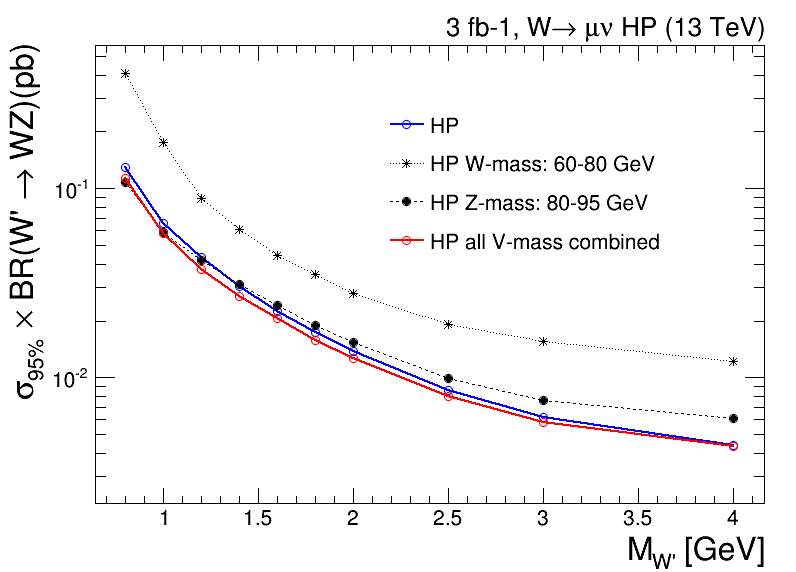
\includegraphics[width=0.49\textwidth]{figures/analysis/search1/AN-15-196/massCategories/compare-HP-HPV-Wprime.png}
  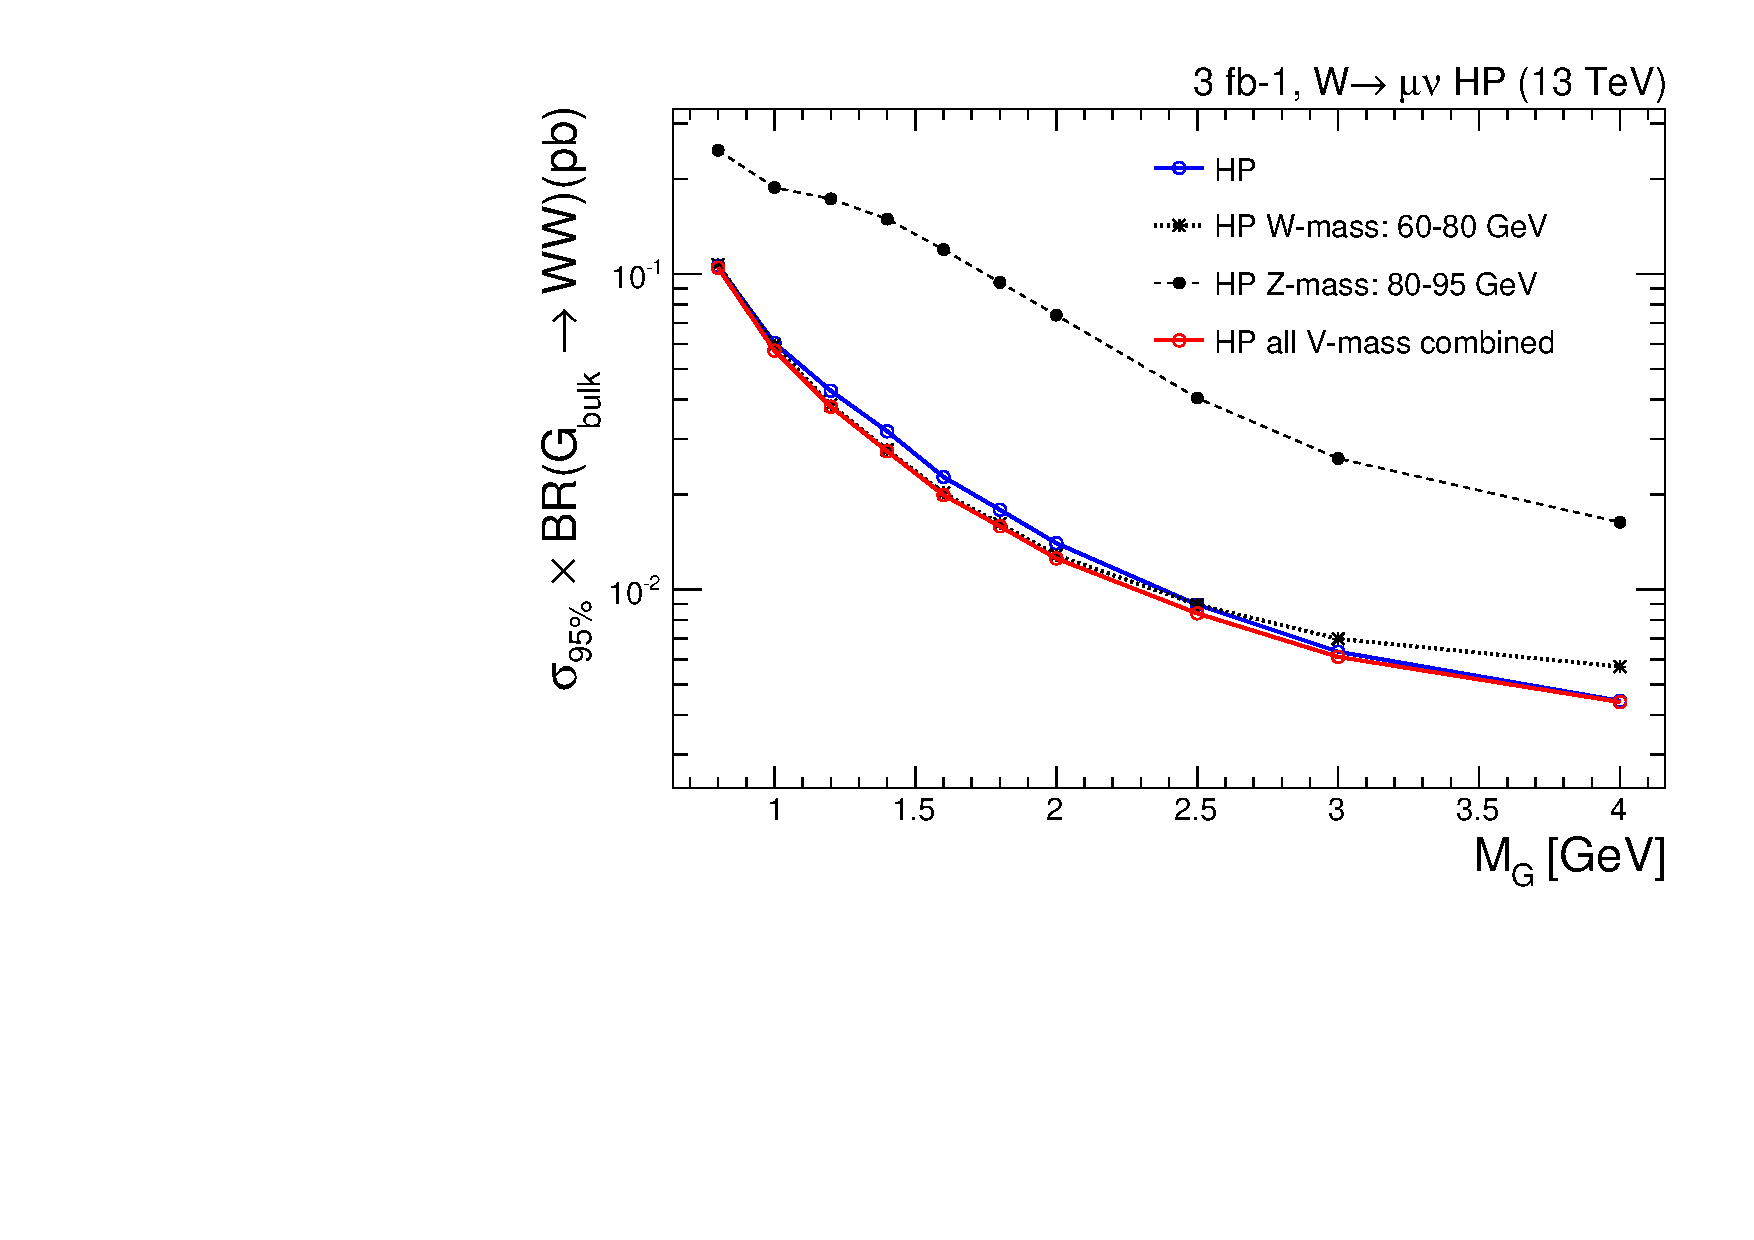
\includegraphics[width=0.49\textwidth]{figures/analysis/search1/AN-15-196/massCategories/compare-HP-HPV-BulkG.pdf}
 \caption{Expected 95\% CL upper limits on the production cross section of a \PWpr (left) and \BulkG (right) signal as function of the resonance mass for the different mass categories for events passing the high-purity $\tau_{21}$ selections.}
 \label{fig:searchI:massCategories}
 \end{figure}

The real benefit of splitting into mass categories becomes obvious when defining a test statistics based on the likelihood ratios of each signal hypothesis, $q = -2 \ln(L_{\BulkG}/L_{\PWpr})$, shown in Figure~\ref{fig:searchI:signalsep}. For a signal with a signal strength corresponding to a 3-4 $\sigma$ excess, the test statistics for each signal hypothesis are well separated ($\sim3.5 \sigma$), allowing us to make a statement of how \BulkG or \PWpr like a possible signal is.

\begin{figure}[h!p]
 \centering
 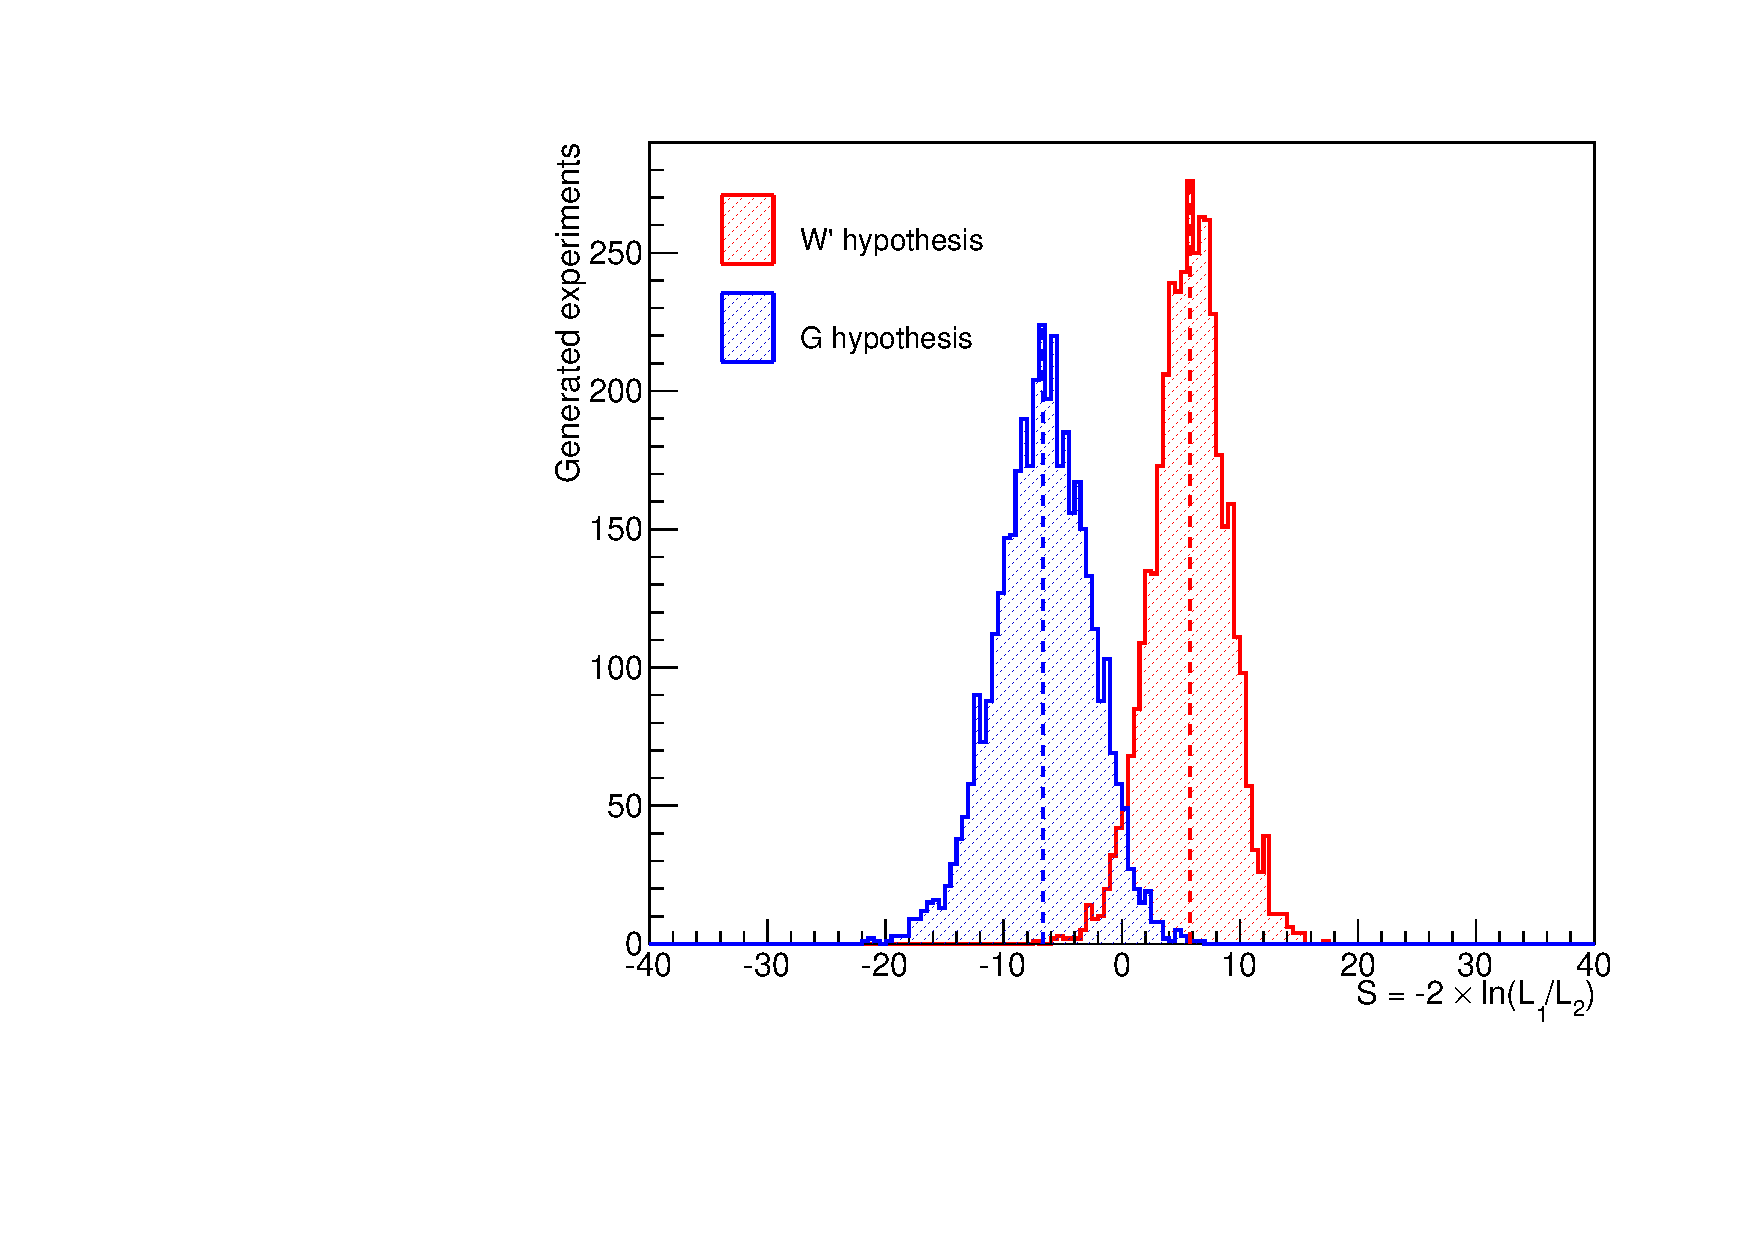
\includegraphics[width=0.49\textwidth]{figures/analysis/search1/AN-15-196/massCategories/sig_sep.pdf}
 \caption{Distribution of the test statistic  $q = -2 \ln(L_{\BulkG}/L_{\PWpr})$ for a \BulkG (blue) and \PWpr signal hypothesis.}
 \label{fig:searchI:signalsep}
 \end{figure}
 
 
With the high-purity and low-purity categories as defined above for each mass window combination, this leaves us with six different signal categories. They are as follows:
\begin{itemize}
\item High-purity, 3 mass categories: \WW, \ZZ and \WZ
\item Low-purity , 3 mass categories: \WW, \ZZ and \WZ
\end{itemize}
In parallel to the mass-category based analysis, we perform an analysis without categorization in mass (similar to the 8 \TeV analysis) as a cross-check. These studies can be found in the Appendix~\ref{app:2015xcheck}.

The final tagging efficiency for different signal hypothesis (top) together with the QCD mistag rate (bottom) in the different signal categories is shown in Figure~\ref{fig:search1:sigeff}. The solid lines represent the tagging efficiency in the full mass window ($65 {\GeV} < M_{p} < 105 {\GeV}$) before splitting into mass categories. A lower signal efficiency the ZZ mass category is observed in all cases. This can be explained from the pruned jet mass distribution on the left in Figure~\ref{fig:wtag}, where a cut at 85 GeV leaves a large fraction of the Z peak in the W mass window. As the main benchmark models under consideration preferably decays to W bosons (in the Bulk Graviton model the branching ratio BR($G_{Bulk}$ $\rightarrow$ \PW\PW) = 2* BR($G_{Bulk}$$\rightarrow$ ZZ), and in the HVT model W'/Z' $\rightarrow$ WZ/WW (but not ZZ) ), a high tagging efficiency for the W boson is preferred. In the limit-setting procedure all the categories are combined and the overall signal efficiency is conserved. For the combined mass-categories (solid line) the signal efficiency is between 16 and 23 \% in the double-tag categories, and between 20 and 34 \% in the single-V tag categories. The mistagging rate in the double-V tag categories is below 1 \% in the high-purity category.

\begin{figure}[h!]
\centering

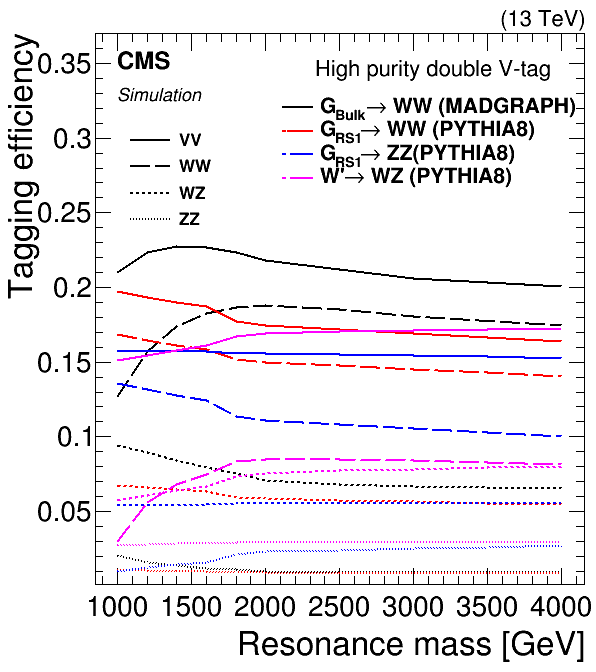
\includegraphics[width=0.49\textwidth]{figures/analysis/search1/AN-15-211/HP_VV_SigEff.png}
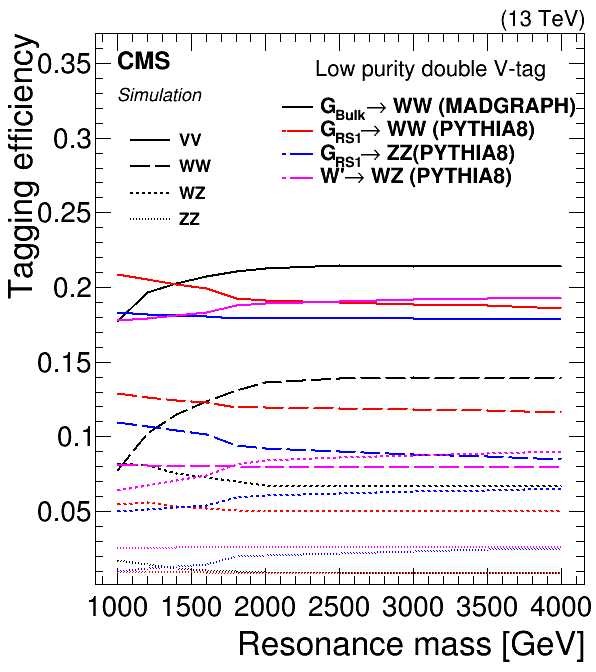
\includegraphics[width=0.49\textwidth]{figures/analysis/search1/AN-15-211/LP_VV_SigEff.png}\\
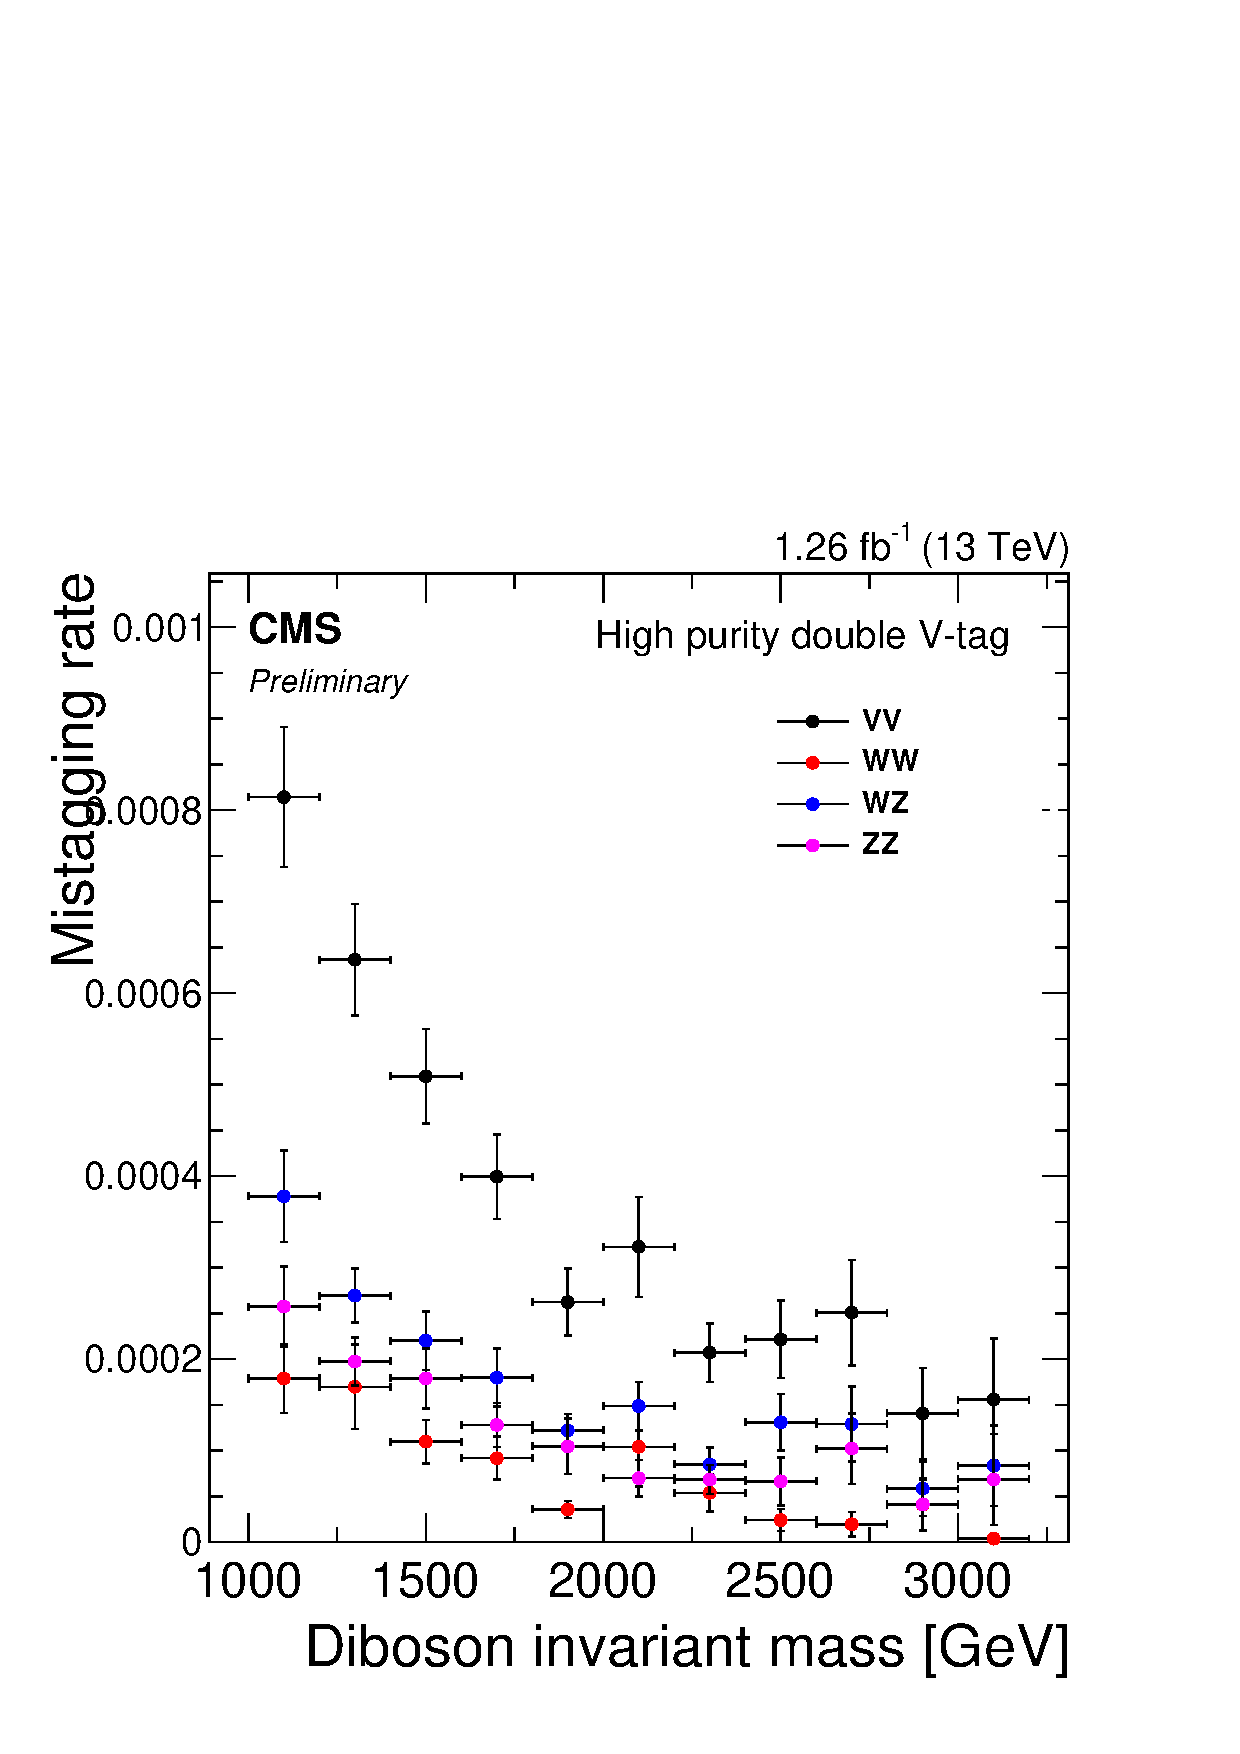
\includegraphics[width=0.49\textwidth]{figures/analysis/search1/AN-15-211/QCD_HP_VV_MistaggingRateEff.pdf}
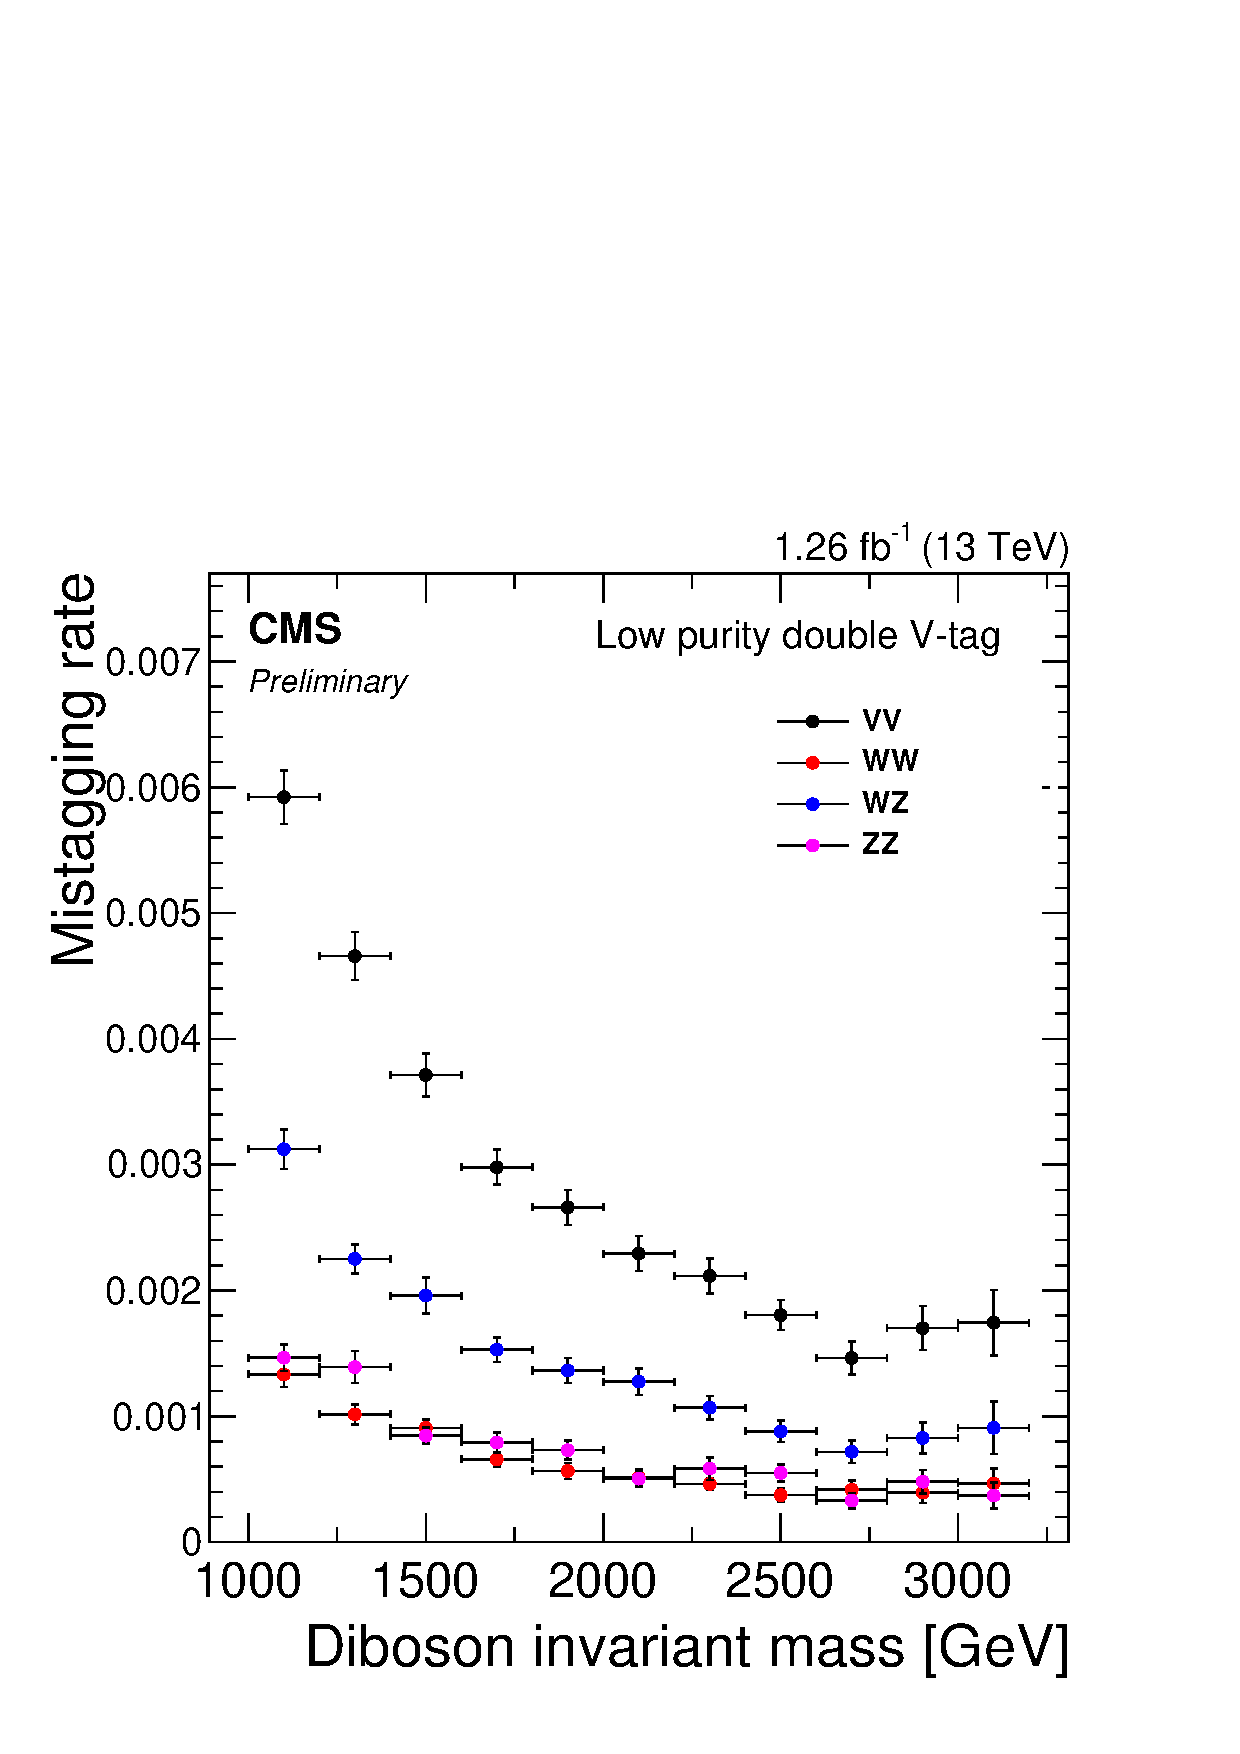
\includegraphics[width=0.49\textwidth]{figures/analysis/search1/AN-15-211/QCD_LP_VV_MistaggingRateEff.pdf}
\caption{Tagging efficiency (top) and mistagging rate (bottom) in the different pruned mass categories in the high-purity category (left) and in the low-purity category (right)}
\label{fig:search1:sigeff}
\end{figure}

The full analysis selections and final categories are listen in Table~\ref{tab:search1:selection}.

\begin{table}[!h!]
\footnotesize
\begin{center}
\label{tab:search1:selection}
\renewcommand{\arraystretch}{1.2}
\begin{tabular}{lc}
\hline 
\multicolumn{1}{c}{Selection} & Value\\
\hline \hline
\multicolumn{1}{c}{Boson selections}\\
\cline{1-1}
V $\to\qqbar$ (2 AK8 jets) & $\pt >200\GeV$\\
  & $|\eta| < 2.4$\\
Pruned jet mass & $65 < {\mJ}_1,{\mJ}_2  < 105\GeV$\\
Topology    & $|\Delta \eta_\mathrm{jj}| < 1.3$\\
Dijet invariant mass     & $\mjj >1\TeV$\\ 
2- to 1-subjettiness ratio    & $\nsubj < 0.75$\\
\hline
%\hline
\multicolumn{1}{c}{\mJ{} categories}\\
\cline{1-1}
WW & $ 65 < {\mJ}_{1} < 85\GeV$, $ 65 < {\mJ}_{2} < 85\GeV$\\
WZ & $ 65 < {\mJ}_{1} < 85\GeV$, $ 85 < {\mJ}_{2} < 105\GeV$\\
ZZ & $ 85 < {\mJ}_{1} < 105\GeV$, $ 85 < {\mJ}_{2} < 105\GeV$\\
\hline
\multicolumn{1}{c}{\nsubj{} categories}\\
\cline{1-1}
High-purity   & $\tau_{\rm{21, jet1}} < 0.45$, $\tau_{\rm{21, jet2}} < 0.45$\\
Low-purity    & $\tau_{\rm{21, jet1}} < 0.45$, $0.45 < \tau_{\rm{21, jet2}} < 0.75$\\
\hline						       
\end{tabular}
\caption{The full analysis selections, mass and \nsubj categories.}
\end{center}
\end{table}


\clearpage
\subsection{Background modeling}
\label{sec:searchI:bkg}

The background modeling in this analysis is based on a smoothness test performed directly on unblinded data, similar to what is done in previous CMS analyses looking for bumps in the dijet invariant mass spectrum~\cite{Chatrchyan:2012ypy,CMS-PAS-EXO-12-059}. We assume that the QCD multijet background in the different analysis categories can be described by smooth, monotonically decreasing functions of 2 or 3 parameters

\begin{equation}
\label{eq:dijet1}
\frac{dN}{d\mjj}= \frac{ P_0 } { (\mjj/\sqrt{s})^{P_2} }\quad\quad\quad{\rm and}
\quad\quad\quad\quad
\frac{dN}{d\mjj}= \frac{ P_0(1-\mjj/\sqrt{s})^{P_1} } { (\mjj/\sqrt{s})^{P_2} }\:\:,
\end{equation}

where $m$ is the dijet invariant mass, $\sqrt{s}$ the centre of mass energy and $P_0$ is a normalization parameter for the probability density function and $P_1$ and $ P_2$ describe the shape. The number of fit parameters is decided through a Fishers F-test~\cite{RePEc:bla:istatr:v:80:y:2012:i:3:p:491-491}. In this test, we start from the 2 parameter function and compare the goodness of fit ($\chi^2$ divided by degrees of freedom) when fitting the data signal region with a 2, 3, 4 and 5 parameter function. We then check at 10\% confidence level (CL) if additional parameters are needed to model the background distribution. The 4 and 5 parameter functions are
\begin{align}
\label{eq:dijet2}
\frac{dN}{d \mjj} &= \frac{ P_0(1-\mjj/\sqrt{s})^{P_1} } {(\mjj/\sqrt{s})^{P_2+P_3\times\log(\mjj/\sqrt{s})} }\\
\frac{dN}{d \mjj} &= \frac{ P_0(1-\mjj/\sqrt{s})^{P_1} } {(\mjj/\sqrt{s})^{P_2+P_3\times\log(\mjj/\sqrt{s})+P_4\times\log(\mjj/\sqrt{s})^2} }
\end{align}

where $P_3$ and $P_4$ are additional free parameters. As an additional cross check, an alternative fit function is also tested:

\begin{equation}
\label{eq:dijet4}
\frac{dN}{d\mjj} = \frac{ P_0(1-\mjj / \sqrt{s}+P_3(\mjj / \sqrt{s})^2)^{P_1} } { (\mjj/\sqrt{s})^{P_2} }.
\end{equation}

The fit range is chosen such that it start where the trigger efficiency has reached its plateau to avoid bias from trigger inefficiency, and extends to the bin after the highest $m_{VV}$ mass point. The binning chosen for the fit follows the detector resolution as in~\cite{Chatrchyan:2012ypy,CMS-PAS-EXO-12-059}.
Before unblinding the signal region, we check that the QCD dijet invariant mass spectrum is expected to be smooth from the distribution in QCD MC as well as exercise the F-test in QCD MC and in a data sideband.\par
The fits to data in the signal region using the different fit functions, are shown in Figure \ref{fig:searchI:fit-dataVV}, and the corresponding F-test output are given in Table \ref{tab:WW_enriched} through Table \ref{tab:ZZ_enriched}. The findings can be summarized as follows: for the WW enriched category a 2 parameter fit is sufficient to describe the data in both the high- and low-purity categories. In the WZ category, a two parameter fit is sufficient in the high-purity category, while three parameters are needed for the low-purity category. For the ZZ category, a 3 parameter fit is needed for both purity categories. The 2 and 3 parameters fit functions as defined in Equation \ref{eq:dijet2} will therefore be used to model the background component in the simultaneous signal and background fit.
\par

\begin{figure}[h!]
\centering
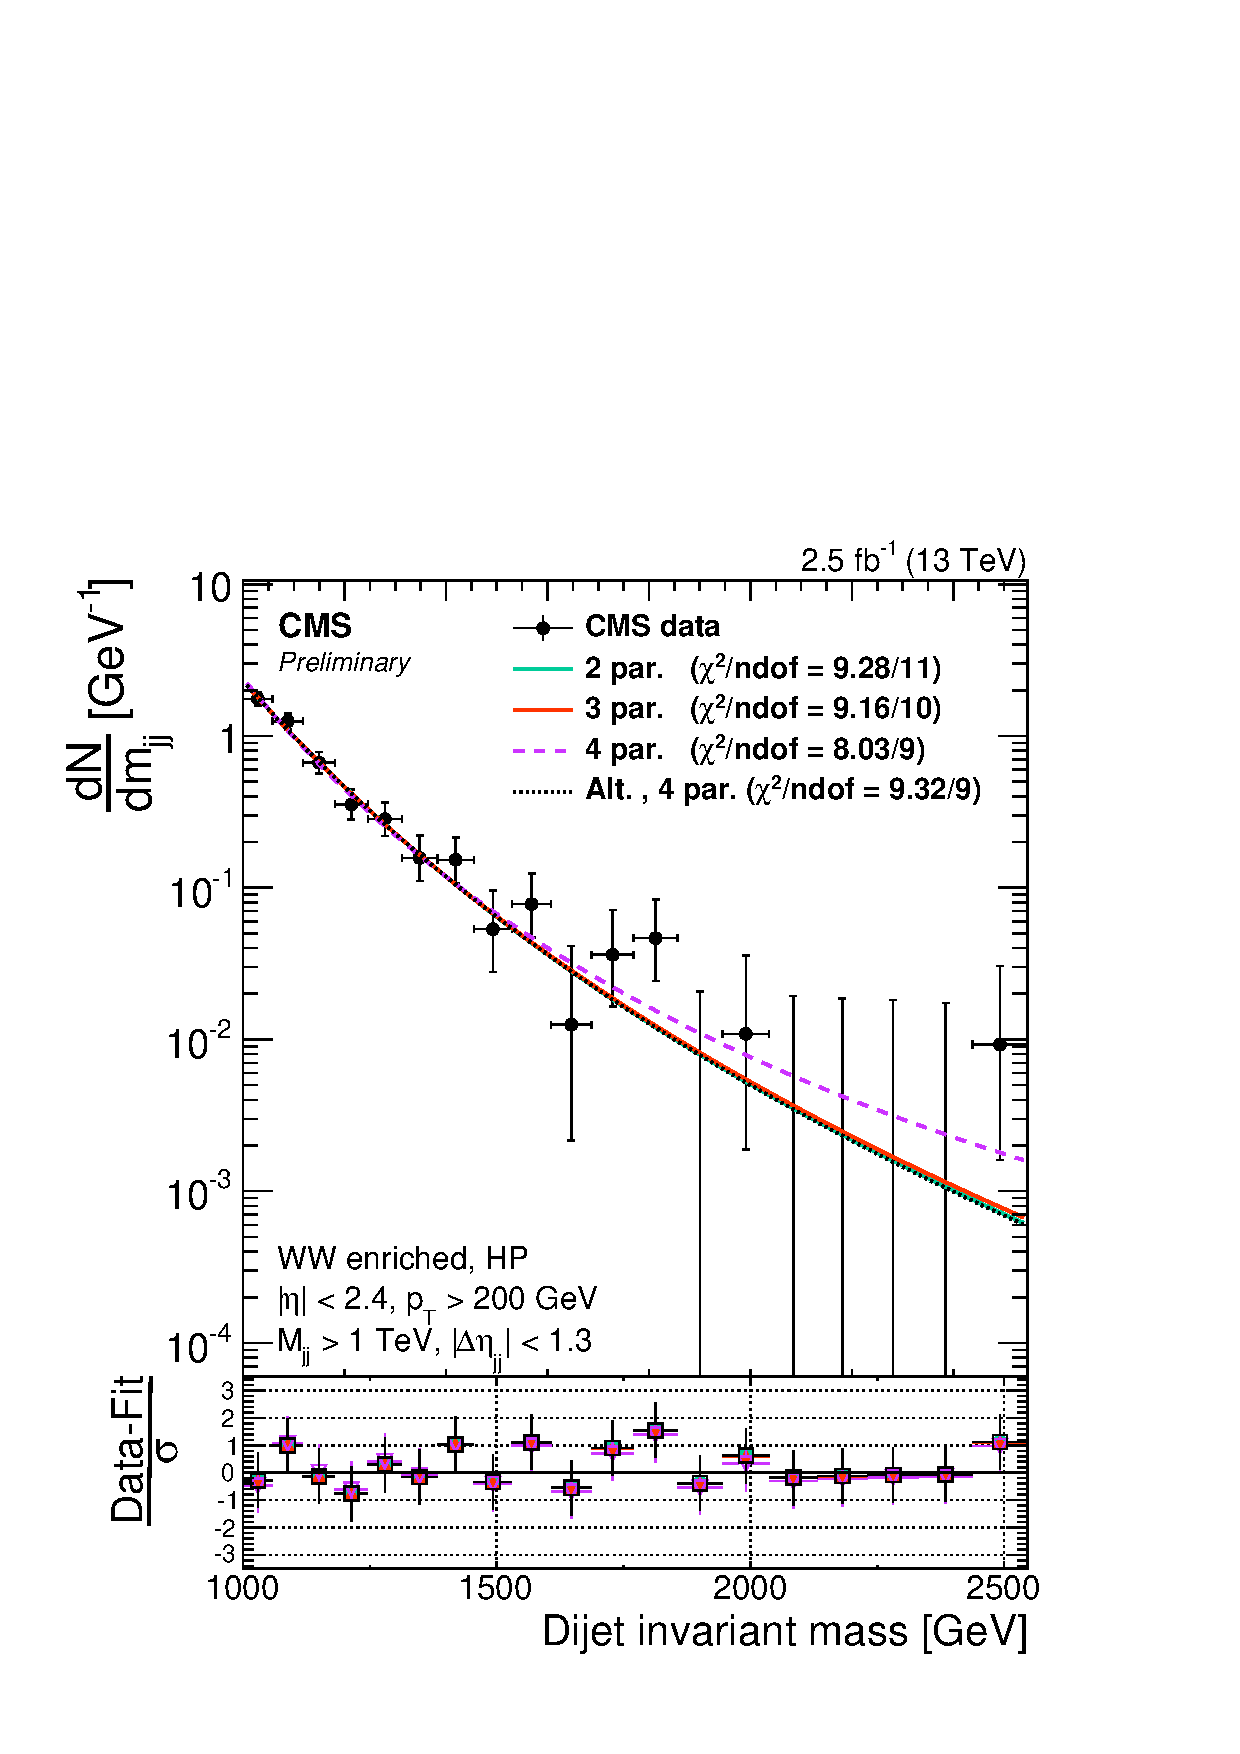
\includegraphics[width=0.43\textwidth]{figures/analysis/search1/AN-15-211/ftest/no5par/WWHP_fitComp.pdf}
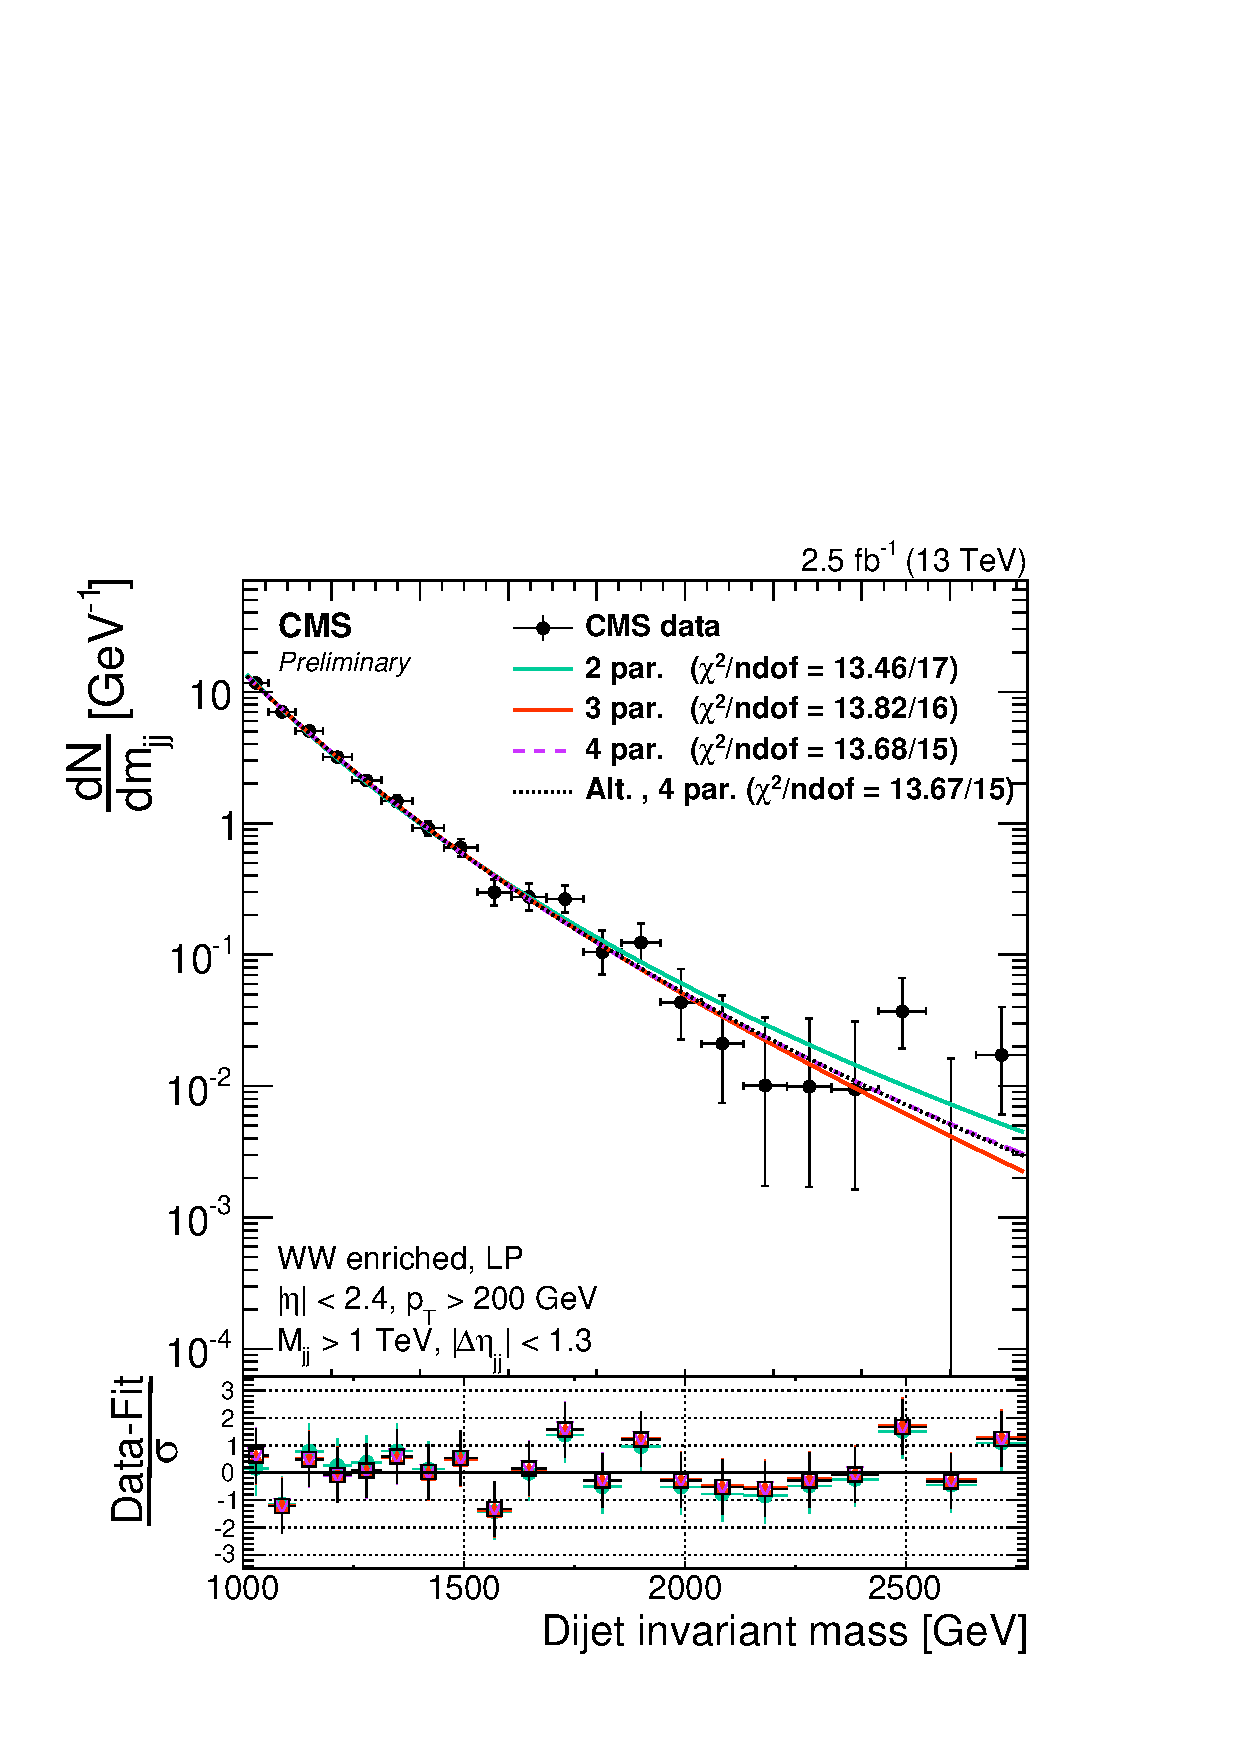
\includegraphics[width=0.43\textwidth]{figures/analysis/search1/AN-15-211/ftest/no5par/WWLP_fitComp.pdf}\\
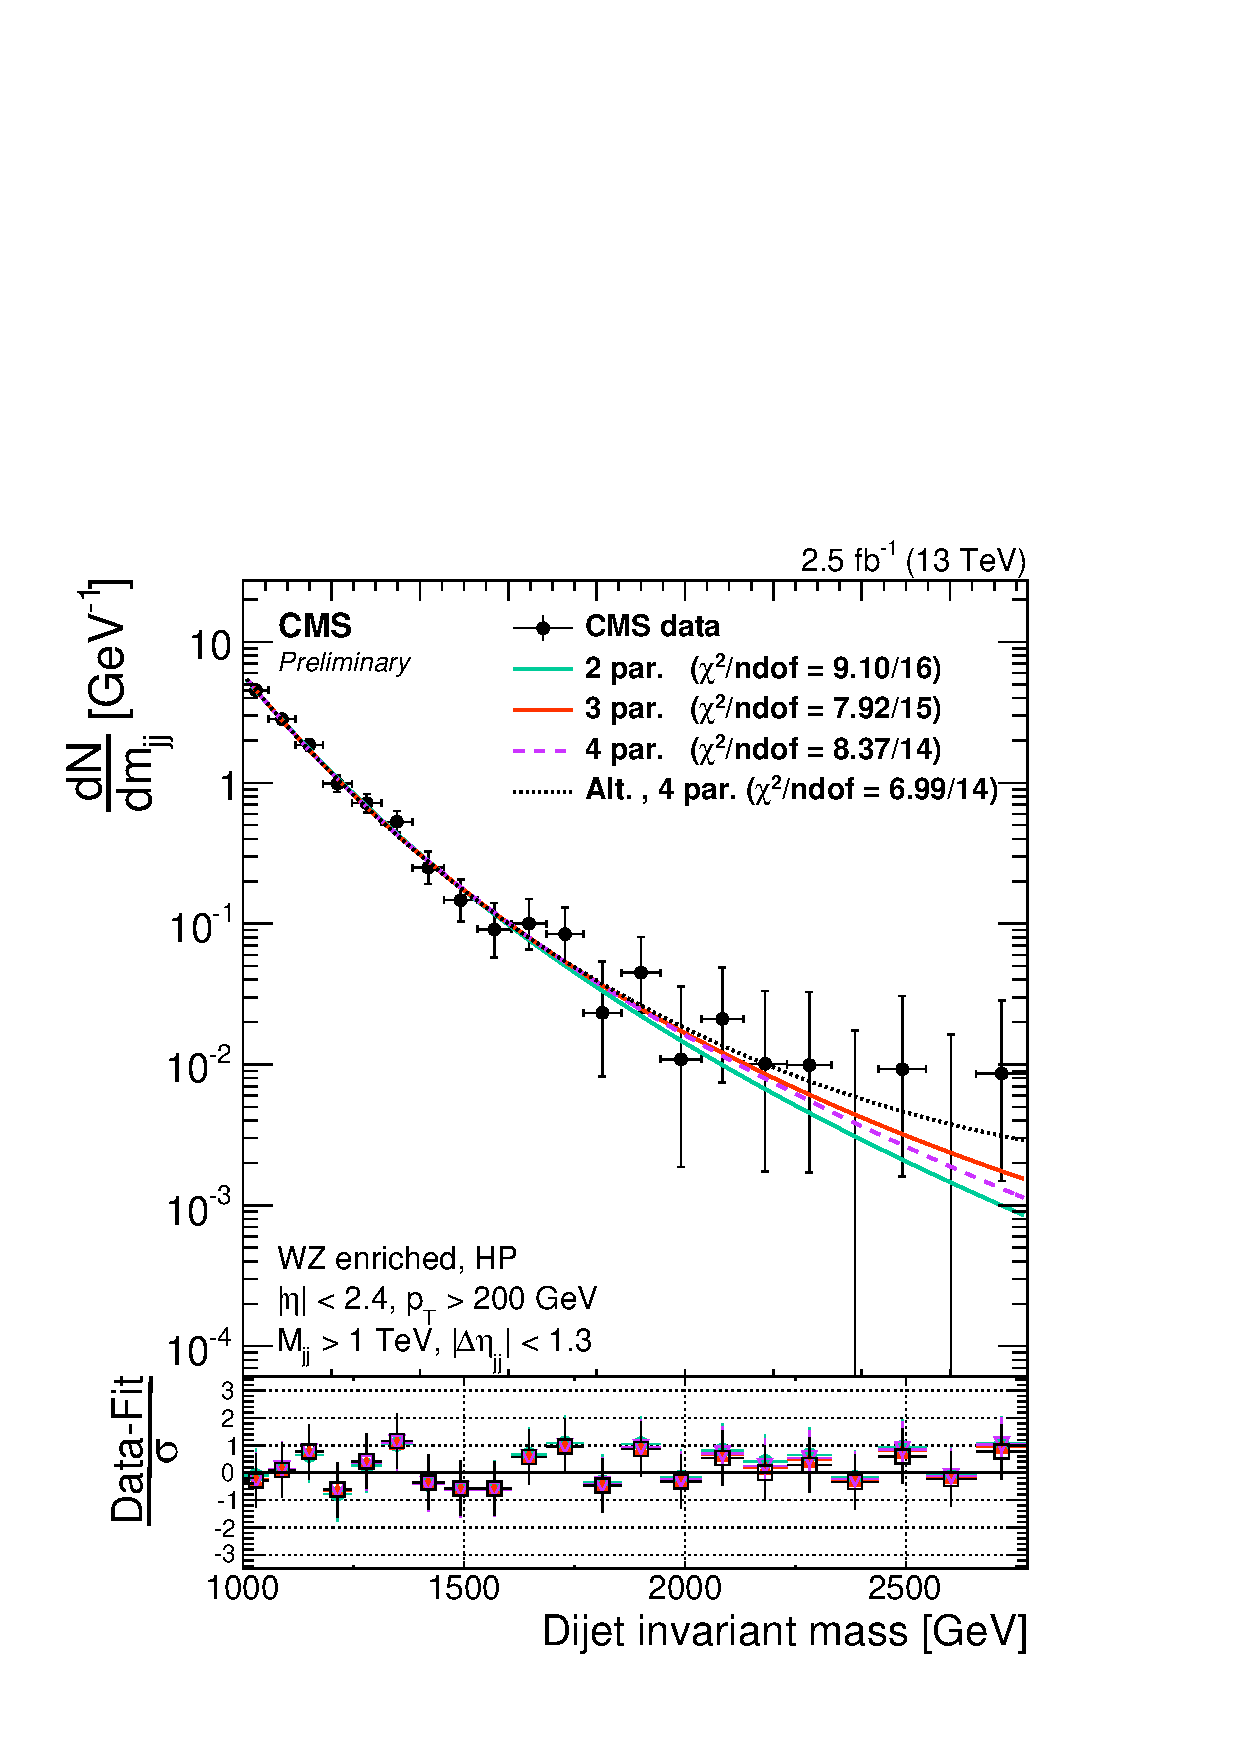
\includegraphics[width=0.43\textwidth]{figures/analysis/search1/AN-15-211/ftest/no5par/WZHP_fitComp.pdf}
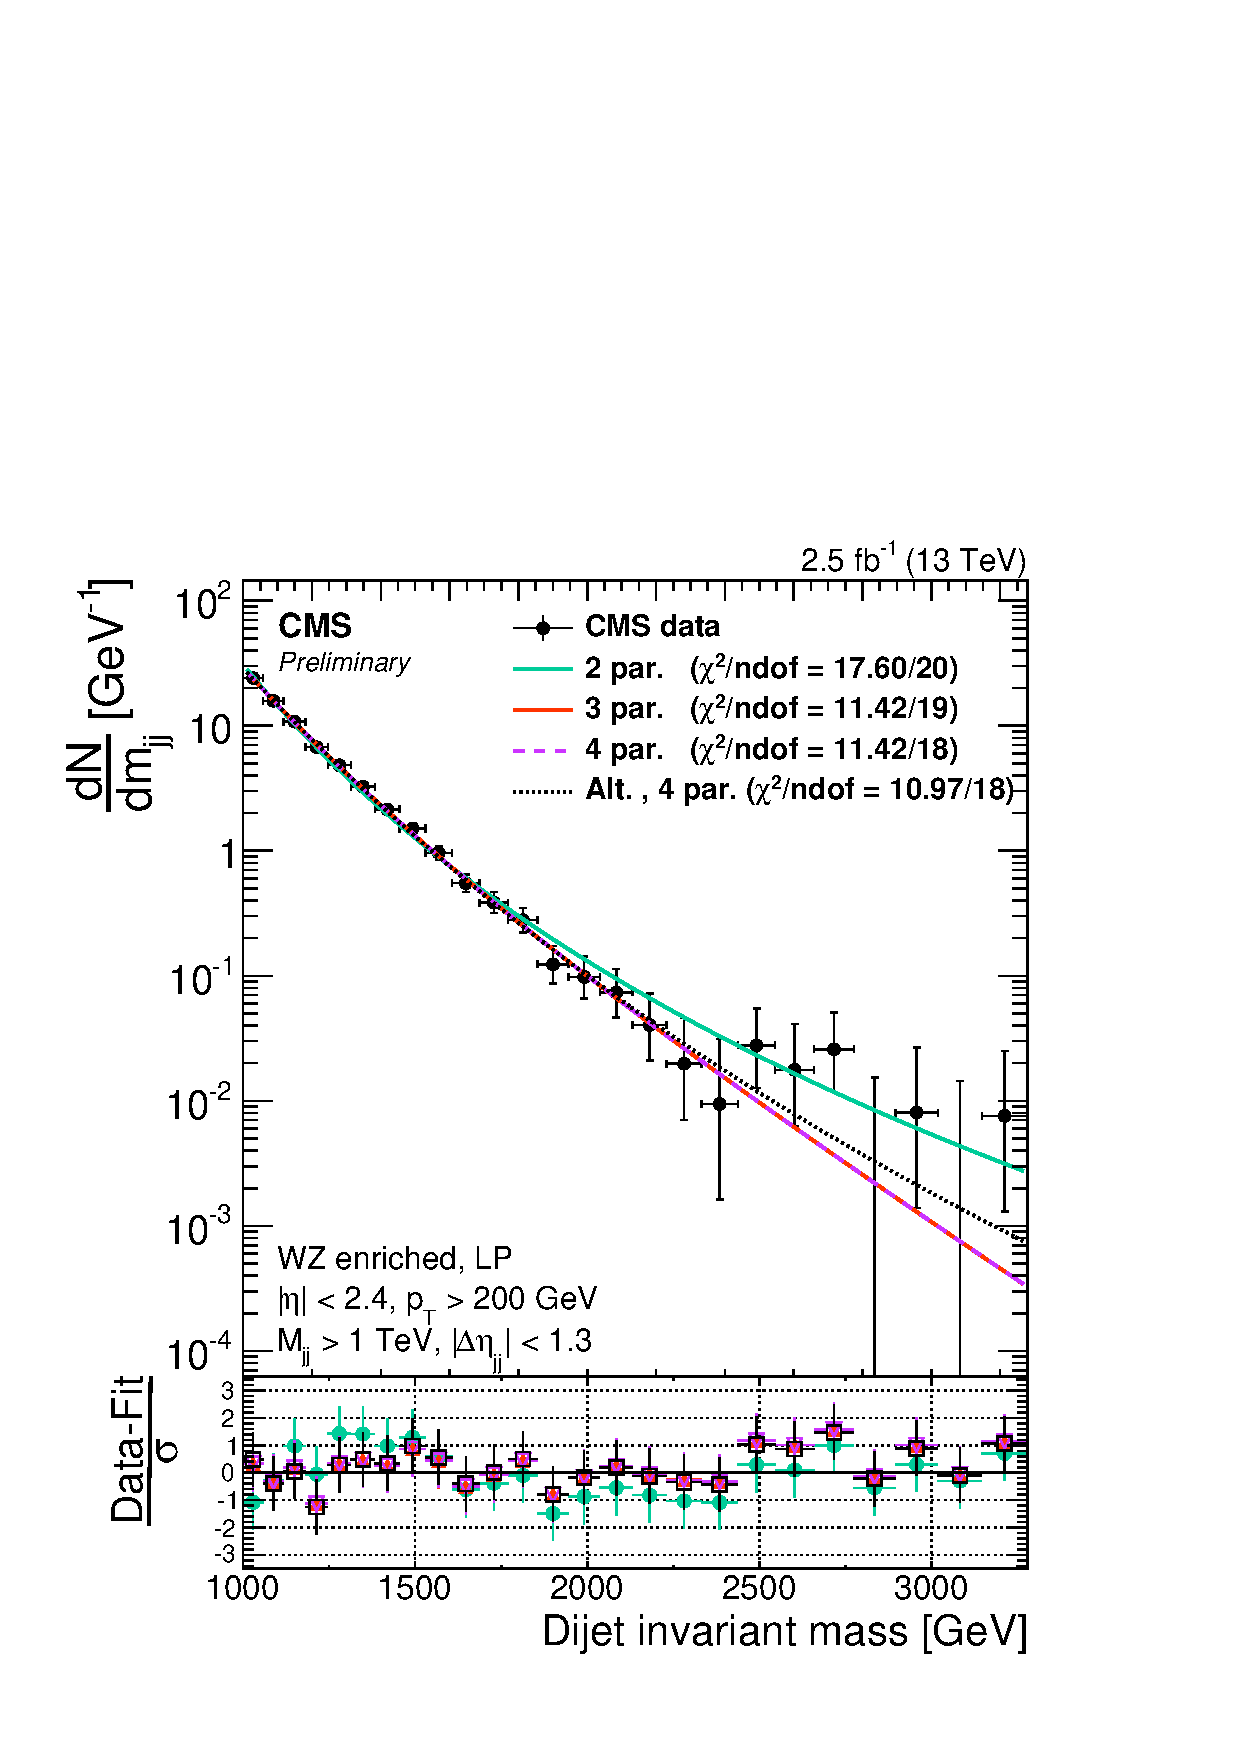
\includegraphics[width=0.43\textwidth]{figures/analysis/search1/AN-15-211/ftest/no5par/WZLP_fitComp.pdf}\\
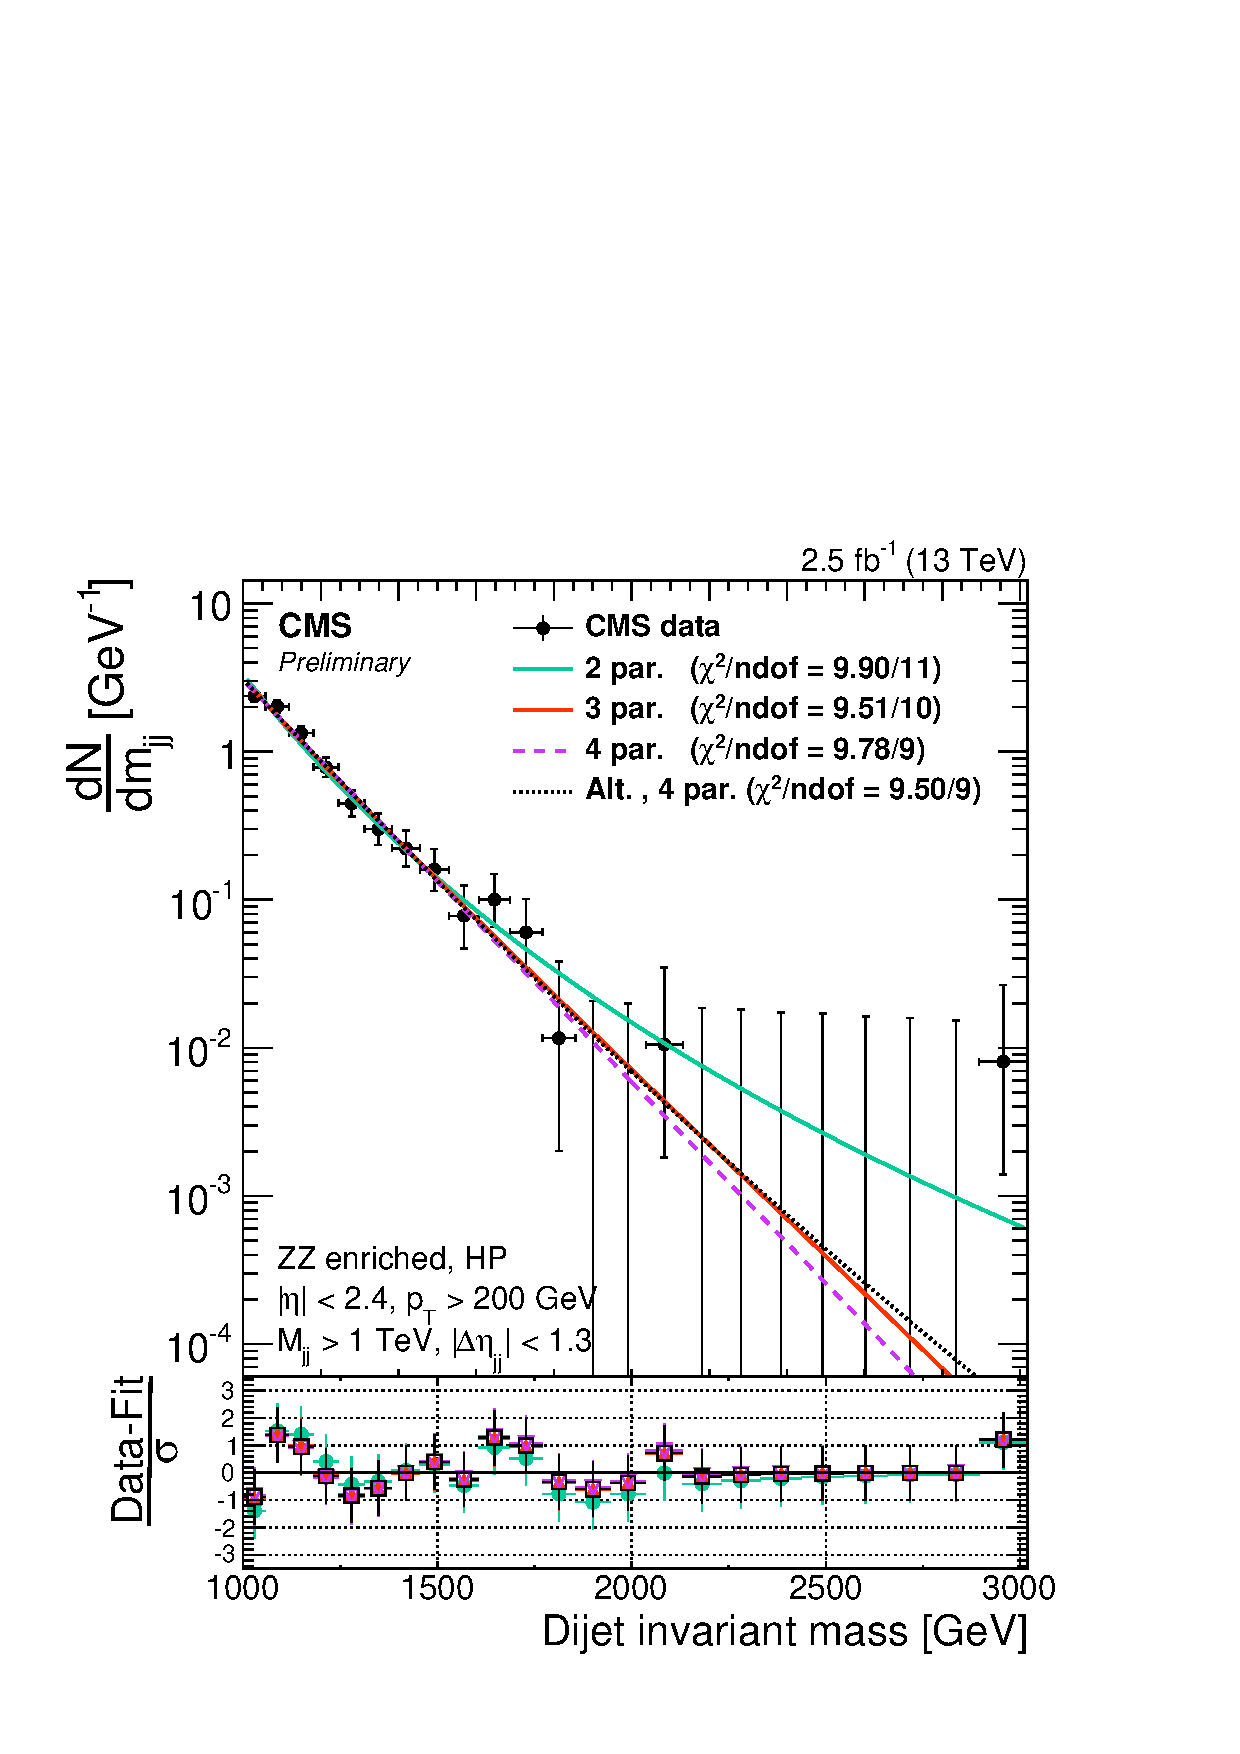
\includegraphics[width=0.43\textwidth]{figures/analysis/search1/AN-15-211/ftest/no5par/ZZHP_fitComp.pdf}
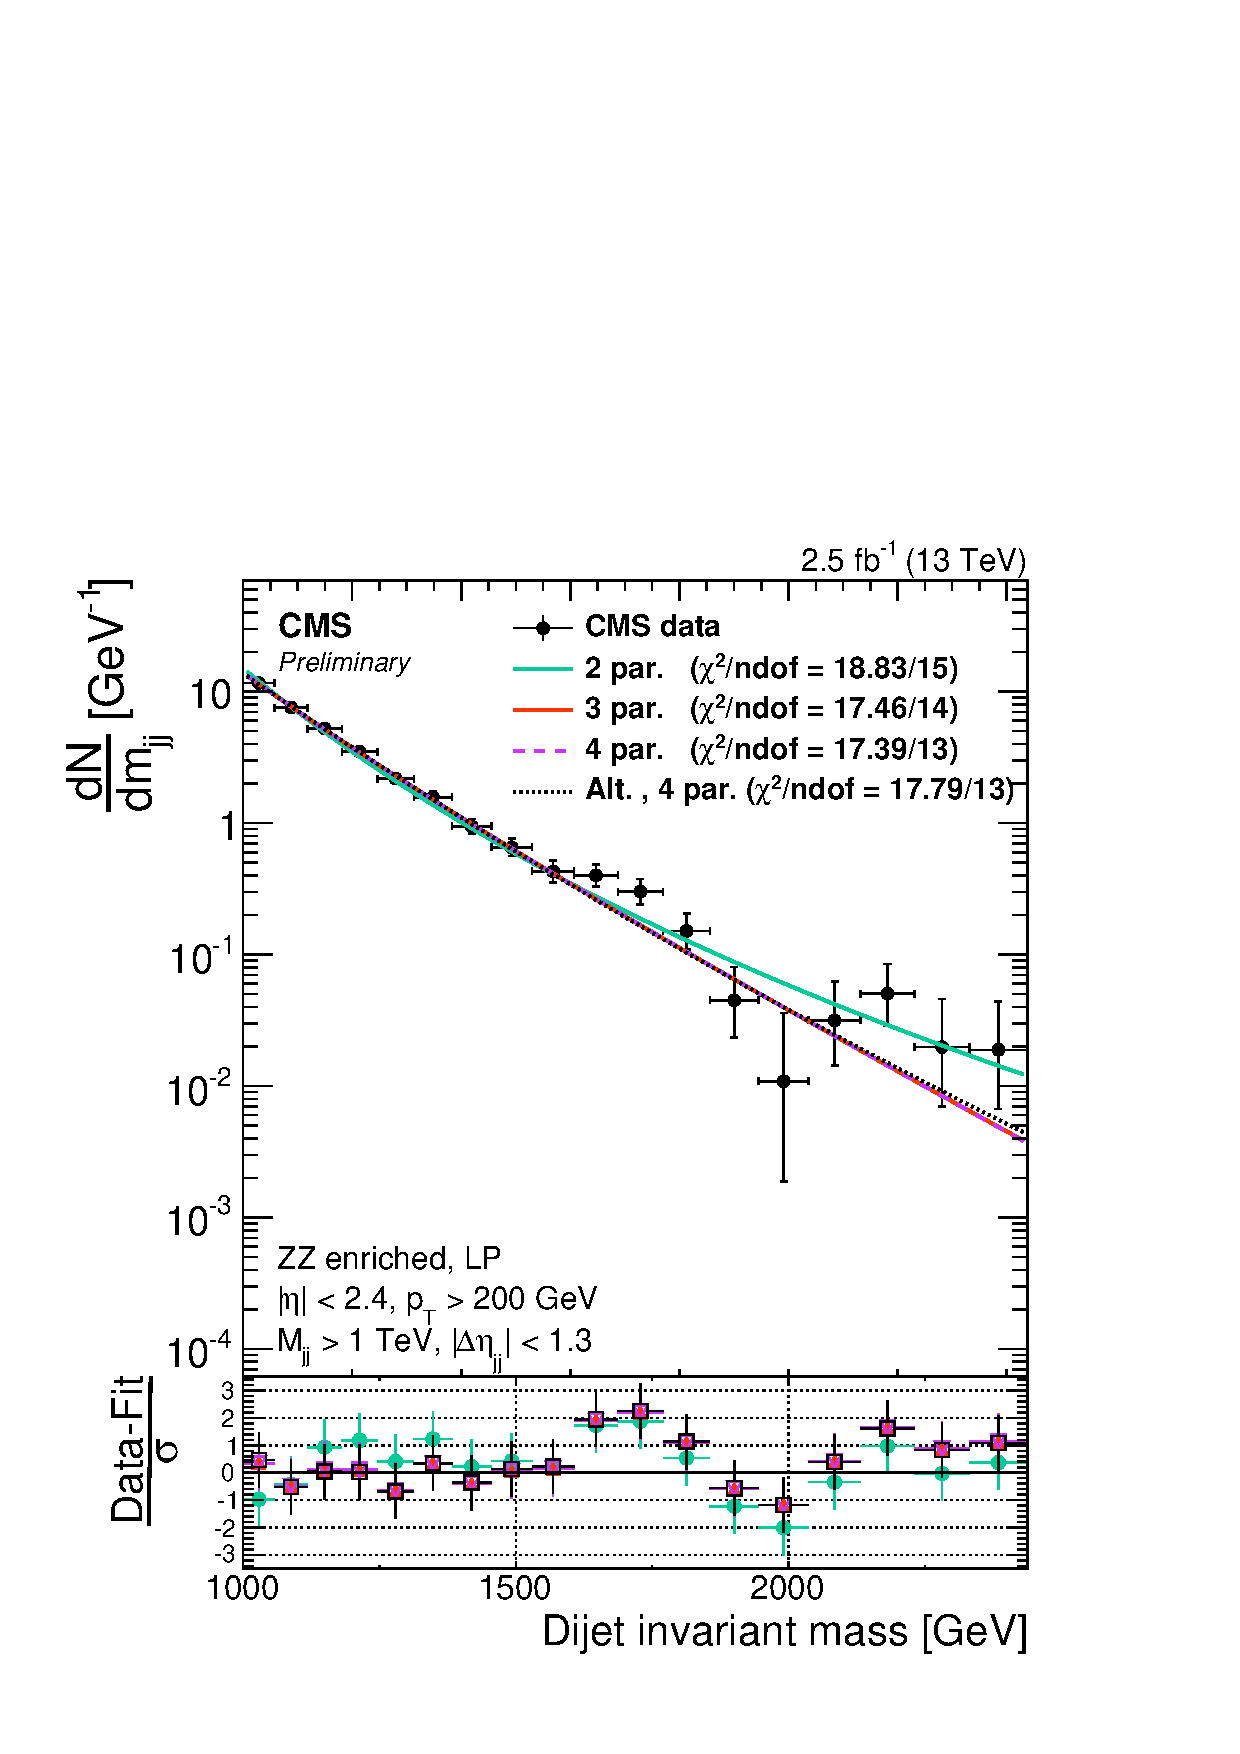
\includegraphics[width=0.43\textwidth]{figures/analysis/search1/AN-15-211/ftest/no5par/ZZLP_fitComp.pdf}\\
\caption{Fitted dijet mass spectrum in the different mass and purity categories in data for the double V-tag category. A 2 parameter fit is sufficient to describe the data for the WW (HP and LP) and WZ (LP) enriched categories. For the ZZ enriched (HP and LP) and WZ (HP) categories, a 3 parameter fit is needed.}
\label{fig:searchI:fit-dataVV}
\end{figure}

\begin{table}[h!]
\centering
\begin{tabular}{|l c c c |}
\hline
\multicolumn{4}{|c|}{WW enriched, HP}\\
\hline
Function & Residuals & $\chi^2$ & ndof \\
\hline
2 par & 0.034 & 9.279 & 11 \\
3 par & 0.034 & 9.160 & 10 \\
4 par & 0.040 & 8.030 & 9 \\
\hline
\hline
Fishers23  & -0.053 &CL &1.0\\
Fishers34  & -1.456 &CL &1.0\\
\hline
\end{tabular}
\quad
\begin{tabular}{|l c c c |}
\hline
\multicolumn{4}{|c|}{WW enriched, LP}\\
\hline
Function & Residuals & $\chi^2$ & ndof \\
\hline
2 par & 0.270 & 13.462 & 17 \\
3 par & 0.300 & 13.819 & 16 \\
4 par & 0.324 & 13.680 & 15 \\
\hline
\hline
Fishers23 & -1.723& CL & 1.0\\
Fishers34 & -1.191& CL & 1.0\\
\hline
\end{tabular}
\caption{Residuals, $\chi^{2}$, and degrees of freedom for the WW enriched HP and LP categories. A 2 parameter fit is needed to describe the data in both categories.}
\label{tab:WW_enriched}
\end{table}


\begin{table}[h!]
\centering
\begin{tabular}{|l c c c |}
\hline
\multicolumn{4}{|c|}{WZ enriched, HP}\\
\hline
Function & Residuals & $\chi^2$ & ndof \\
\hline
2 par & 0.039 & 9.105 & 16 \\
3 par & 0.047 & 7.915 & 15 \\
4 par & 0.048 & 8.370 & 14 \\
\hline
\hline
Fishers23 & -2.598& CL & 1.0\\
Fishers34 & -0.491& CL & 1.0\\
\hline
\end{tabular}
\quad
\begin{tabular}{|l c c c |}
\hline
\multicolumn{4}{|c|}{WZ enriched, LP}\\
\hline
Function & Residuals & $\chi^2$ & ndof \\
\hline
2 par & 1.016 & 17.602 & 20 \\
3 par & 0.270 & 11.424 & 19 \\
4 par & 0.269 & 11.421 & 18 \\
\hline
\hline
Fishers23 & 55.258& CL & 0.0\\
Fishers34 & 0.078& CL & 0.783\\
\hline
\end{tabular}
\caption{Residuals, $\chi^{2}$, and degrees of freedom for the WZ enriched HP (left) and LP (right) categories. A 2 parameter fit is sufficient to describe the data in the high-purity category, while three parameters are needed for the low-purity category.}
\label{tab:WZ_enriched}
\end{table}



\begin{table}[h!]
\centering
\begin{tabular}{|l c c c |}
\hline
\multicolumn{4}{|c|}{ZZ enriched, HP}\\
\hline
Function & Residuals & $\chi^2$ & ndof \\
\hline
2 par & 0.220 & 9.901 & 11 \\
3 par & 0.140 & 9.511 & 10 \\
4 par & 0.124 & 9.781 & 9 \\
\hline
\hline
Fishers23 & 6.302& CL & 0.029\\
Fishers34 & 1.246& CL & 0.290\\
\hline
\end{tabular}
\quad
\begin{tabular}{|l c c c |}
\hline
\multicolumn{4}{|c|}{ZZ enriched, LP}\\
\hline
Function & Residuals & $\chi^2$ & ndof \\
\hline
2 par & 0.448 & 18.832 & 15 \\
3 par & 0.121 & 17.463 & 14 \\
4 par & 0.118 & 17.394 & 13 \\
\hline
\hline
Fishers23 & 40.438& CL & 0.0\\
Fishers34 & 0.356& CL & 0.56\\
\hline
\end{tabular}
\caption{Residuals, $\chi^{2}$, and degrees of freedom for the ZZ enriched LP and HP categories. A 3 parameter fit is sufficient to describe the data in both categories.}
\label{tab:ZZ_enriched}
\end{table}

\clearpage
\subsection{Signal modeling}
\label{sec:searchI:sig}

The signal shape is extracted from signal MC with masses in the range from 1 to 4 TeV. A linear interpolation provides shapes for the mass points in between in steps of 100 GeV. From these shapes, pdf models are constructed as composite models with a Gaussian core due to detector resolution and an exponential tail to account for parton distribution function effects. Parametric shape uncertainties due to jet energy scale and resolution uncertainties are inserted by variations of the Gaussian peak position and width. The dijet invariant mass shape for different benchmark model signals are shown in Figure \ref{fig:sigfit}. The signal and background components are then simultaneously fitted to the data points.

\begin{figure}[h!]
\centering
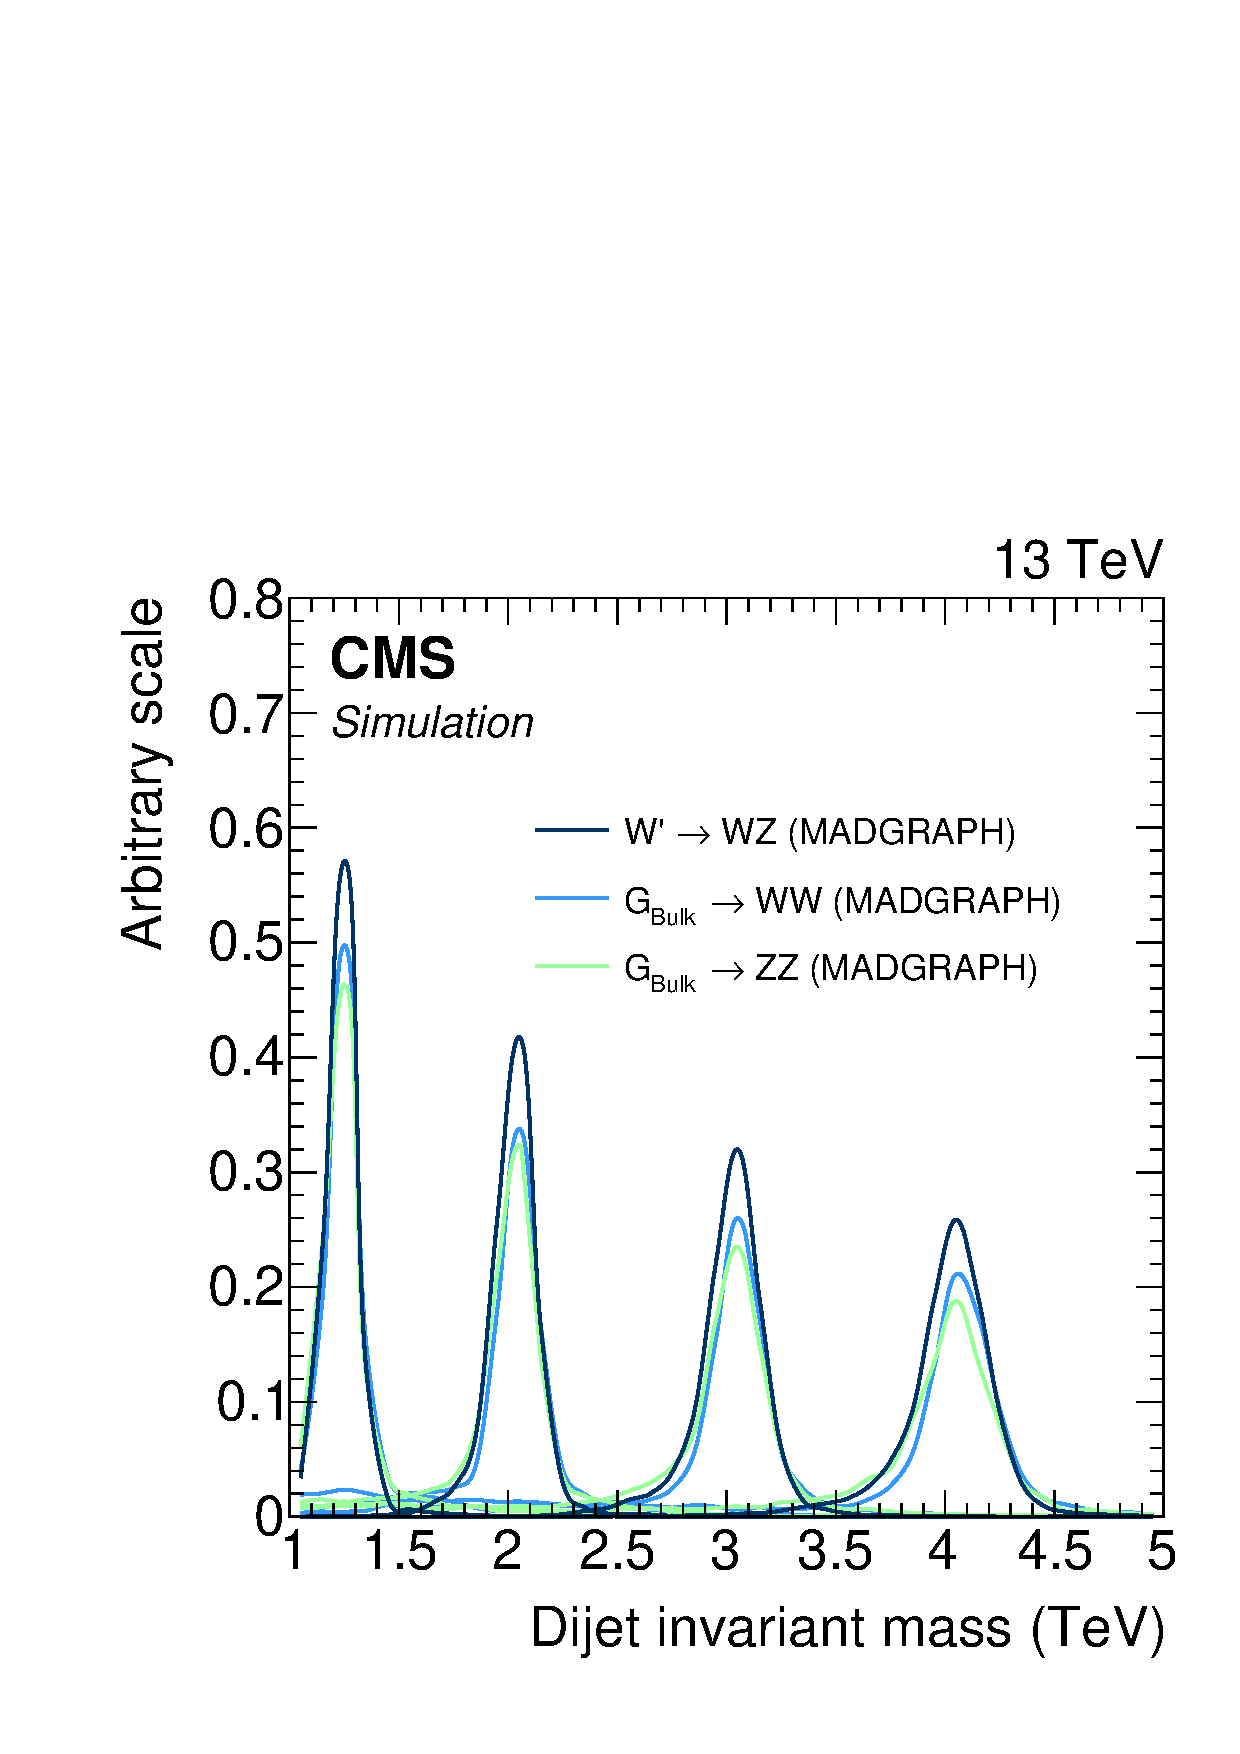
\includegraphics[width=0.49\textwidth]{figures/analysis/search1/B2G-16-004/Figure_005-a.pdf}
\caption{Dijet invariant mass from signal MC used to extract the signal shape. Here for 1.2, 2, 3 and 4 TeV resonances.}
\label{fig:searchI:fit-dataVV}
\end{figure}

\subsection{Systematic uncertainties}
\label{sec:searchI:sys}
TODO!!

\clearpage

\subsection{Results}
\label{sec:searchI:results}
The background fits for each analysis category in the data signal region are shown in Figure \ref{fig:search1:bkgfitMassCat}. Here a background only fit is performed while, as described above, a simultaneous fit is used for the limit setting procedure. The filled area correspond to the 1 sigma error band of the background fit, obtained using linear error propagation.

\begin{figure}[h!]
\centering
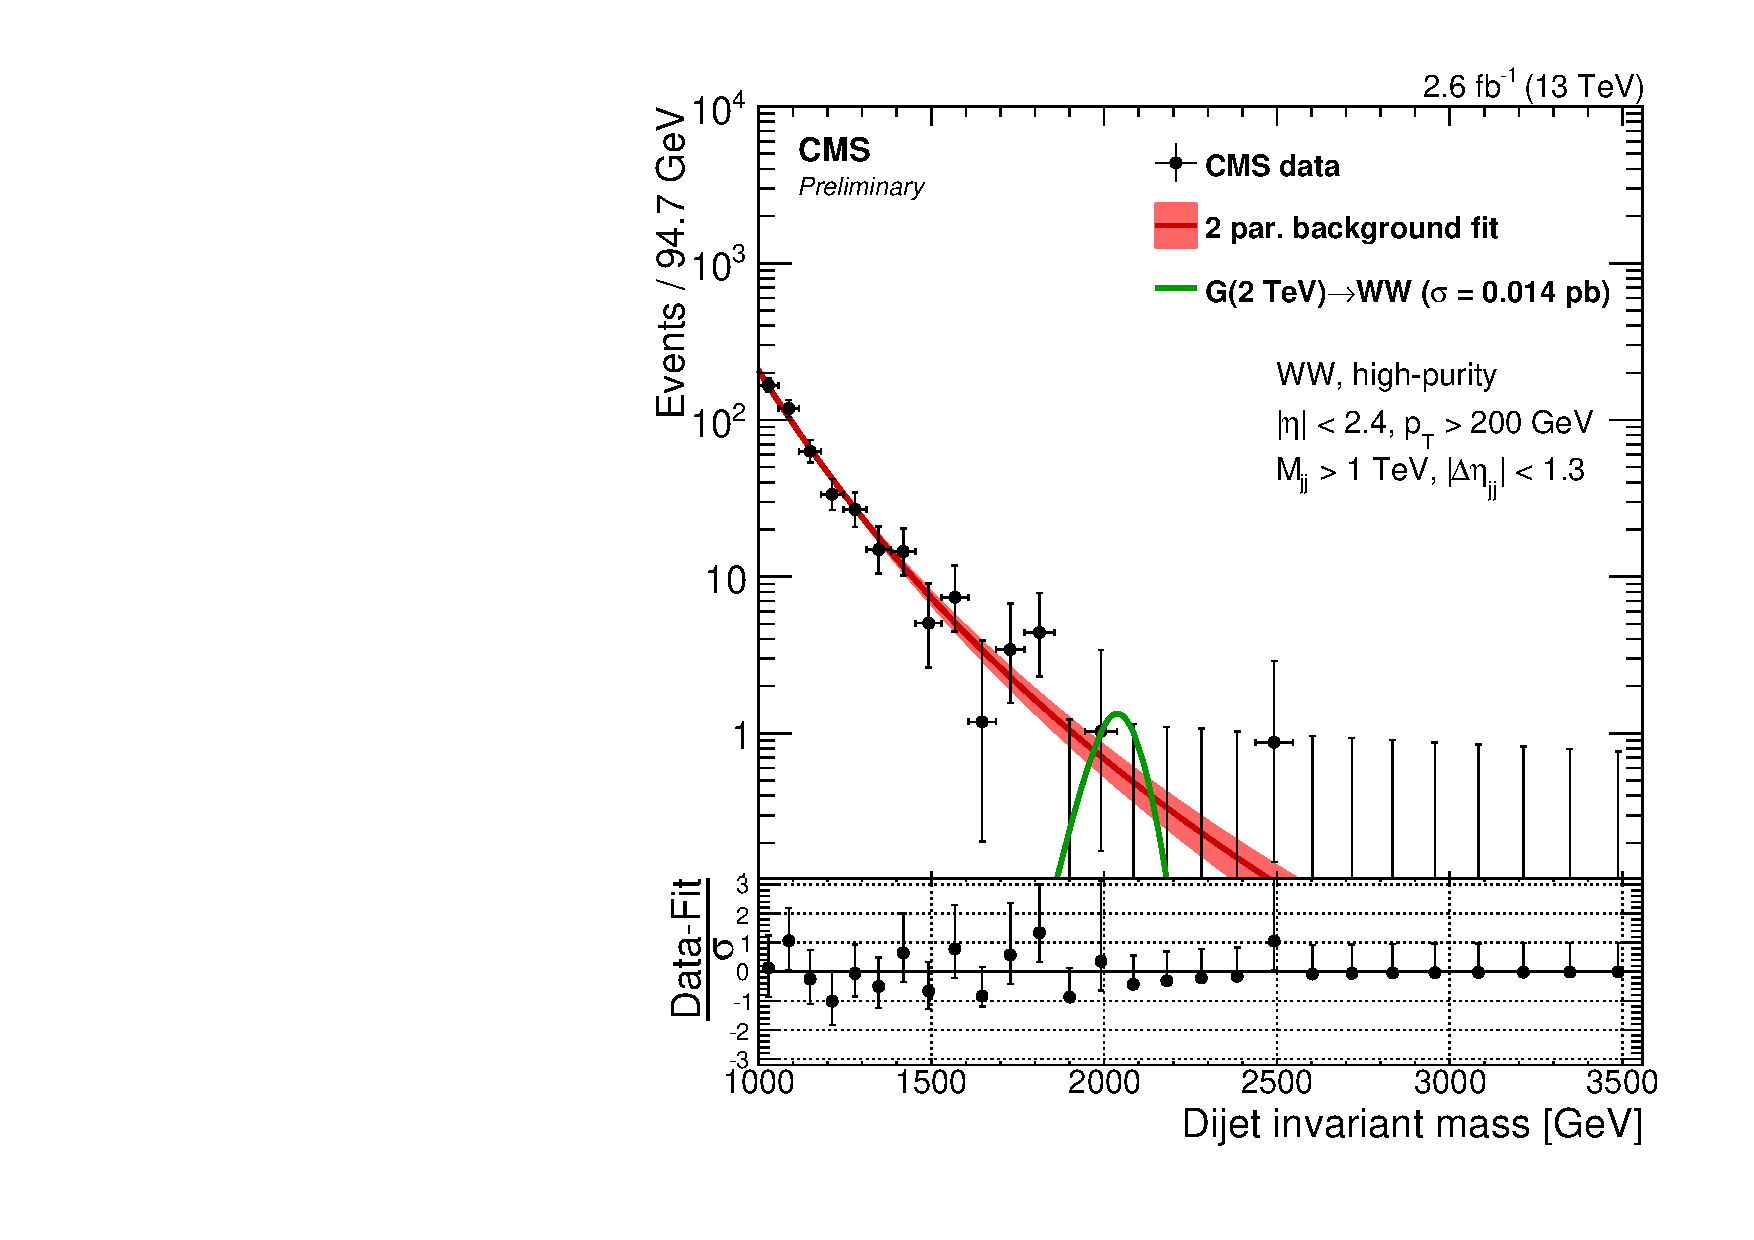
\includegraphics[width=0.44\textwidth]{figures/analysis/search1/AN-15-211/fits/MLfits/BkgFit_DijetMassHighPuriWW.pdf}
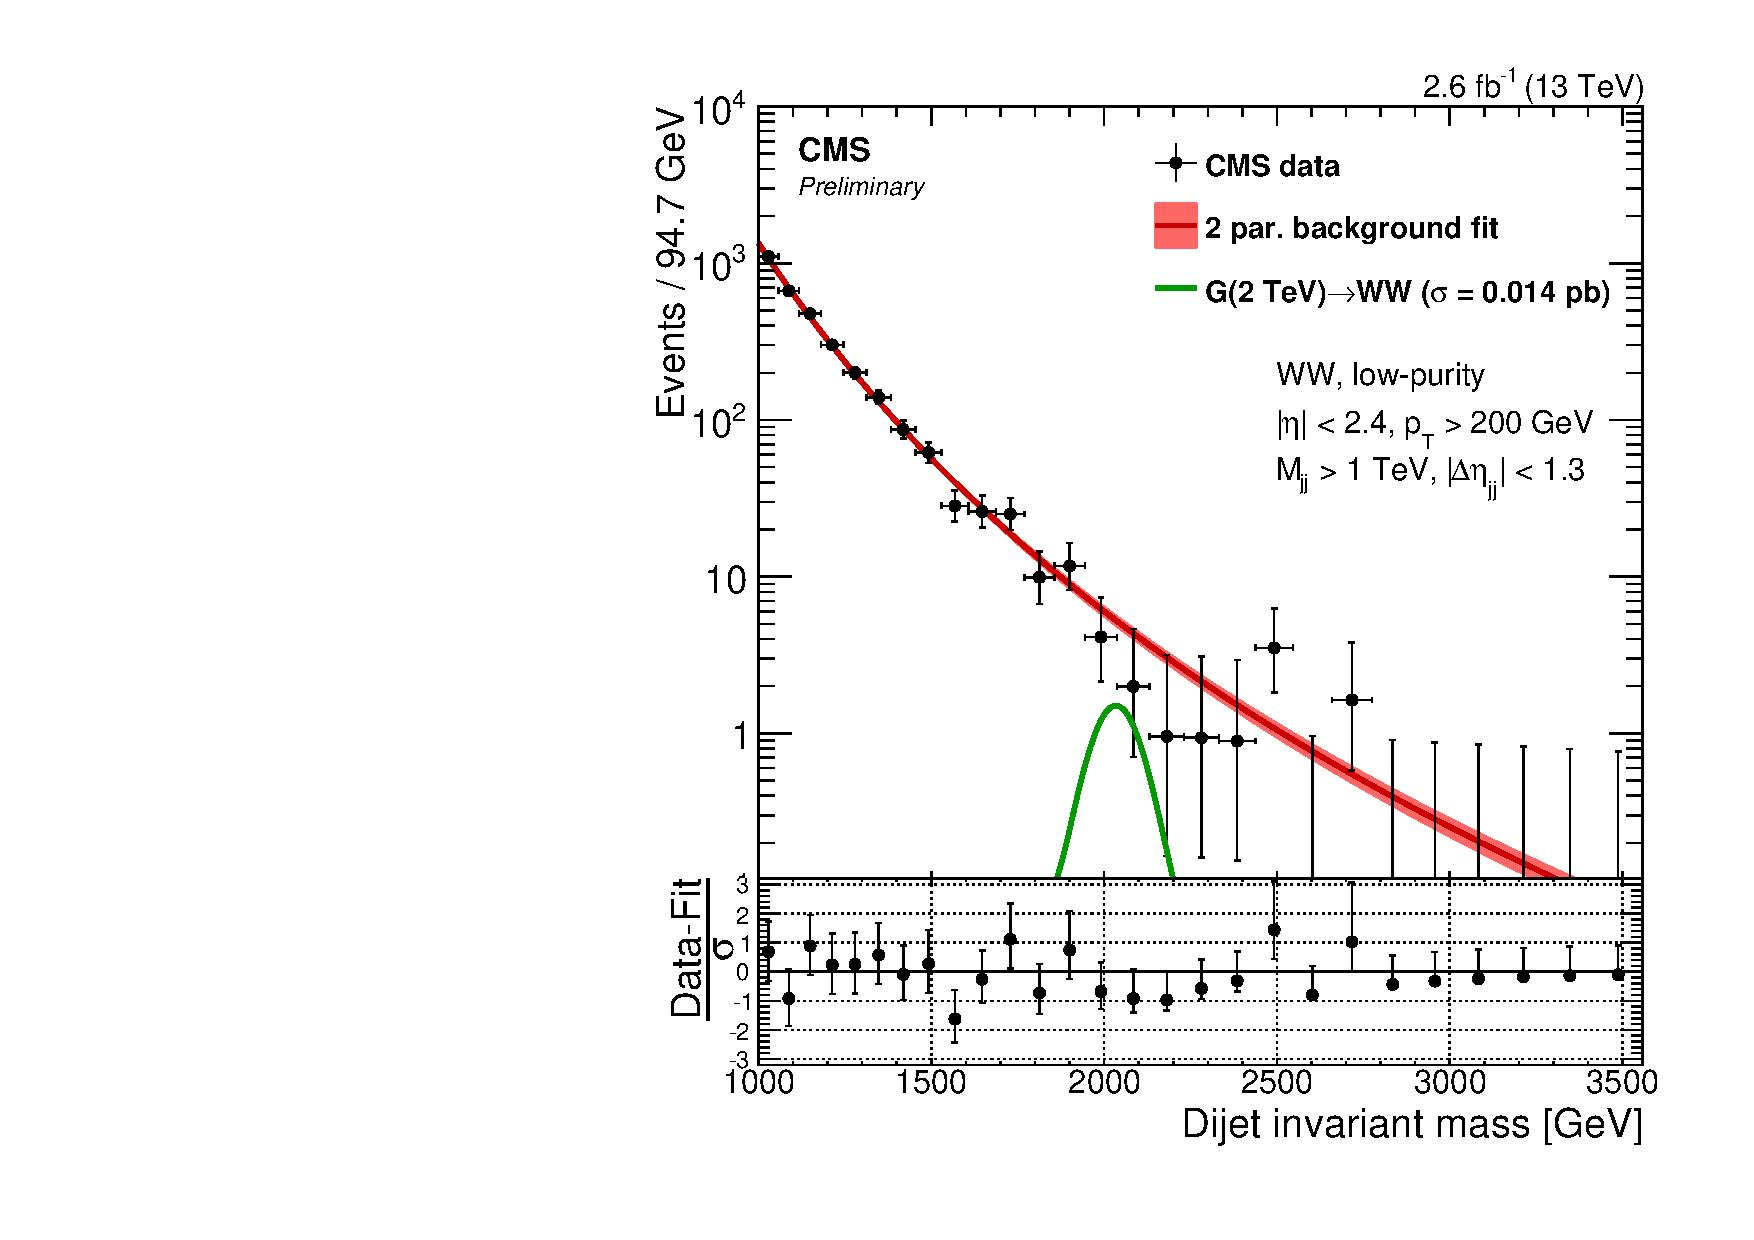
\includegraphics[width=0.44\textwidth]{figures/analysis/search1/AN-15-211/fits/MLfits/BkgFit_DijetMassLowPuriWW.pdf}\\
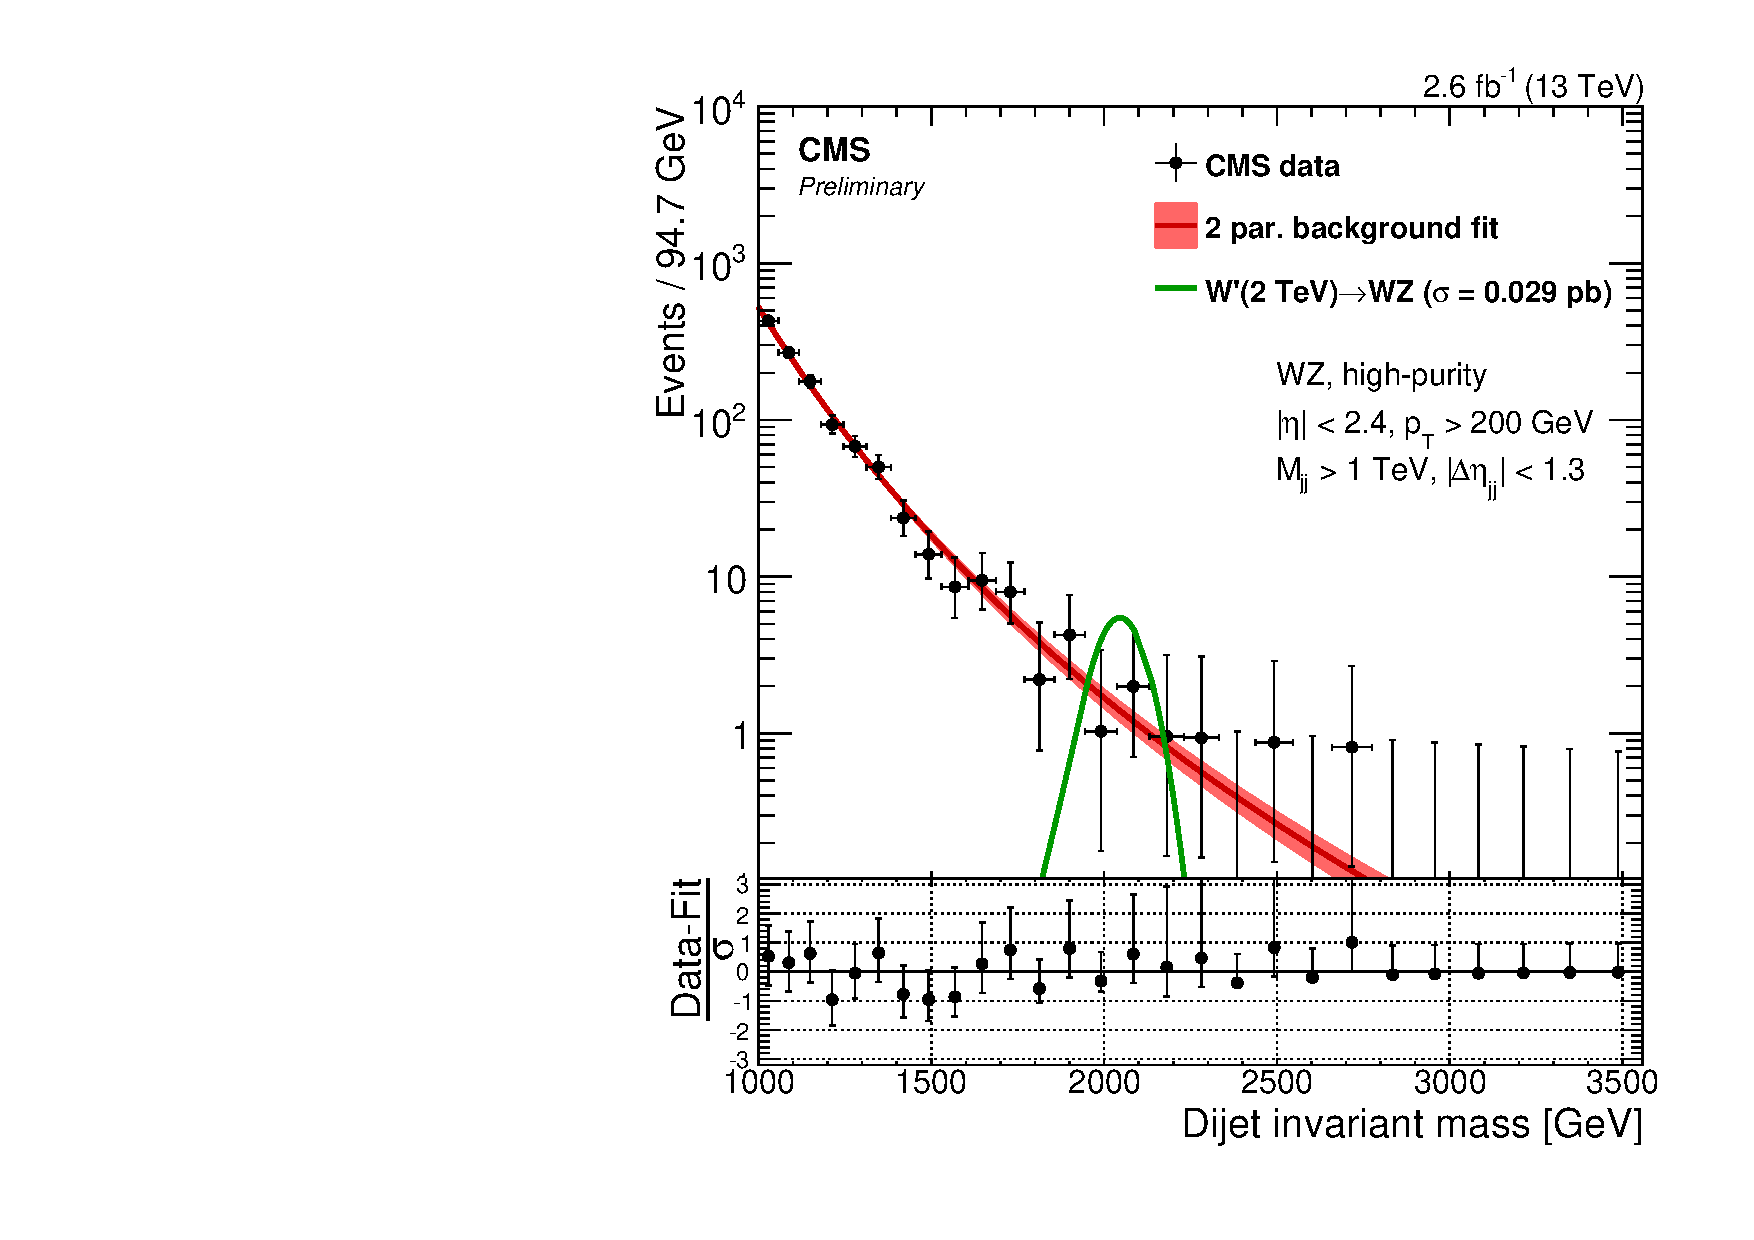
\includegraphics[width=0.44\textwidth]{figures/analysis/search1/AN-15-211/fits/MLfits/BkgFit_DijetMassHighPuriWZ.pdf}
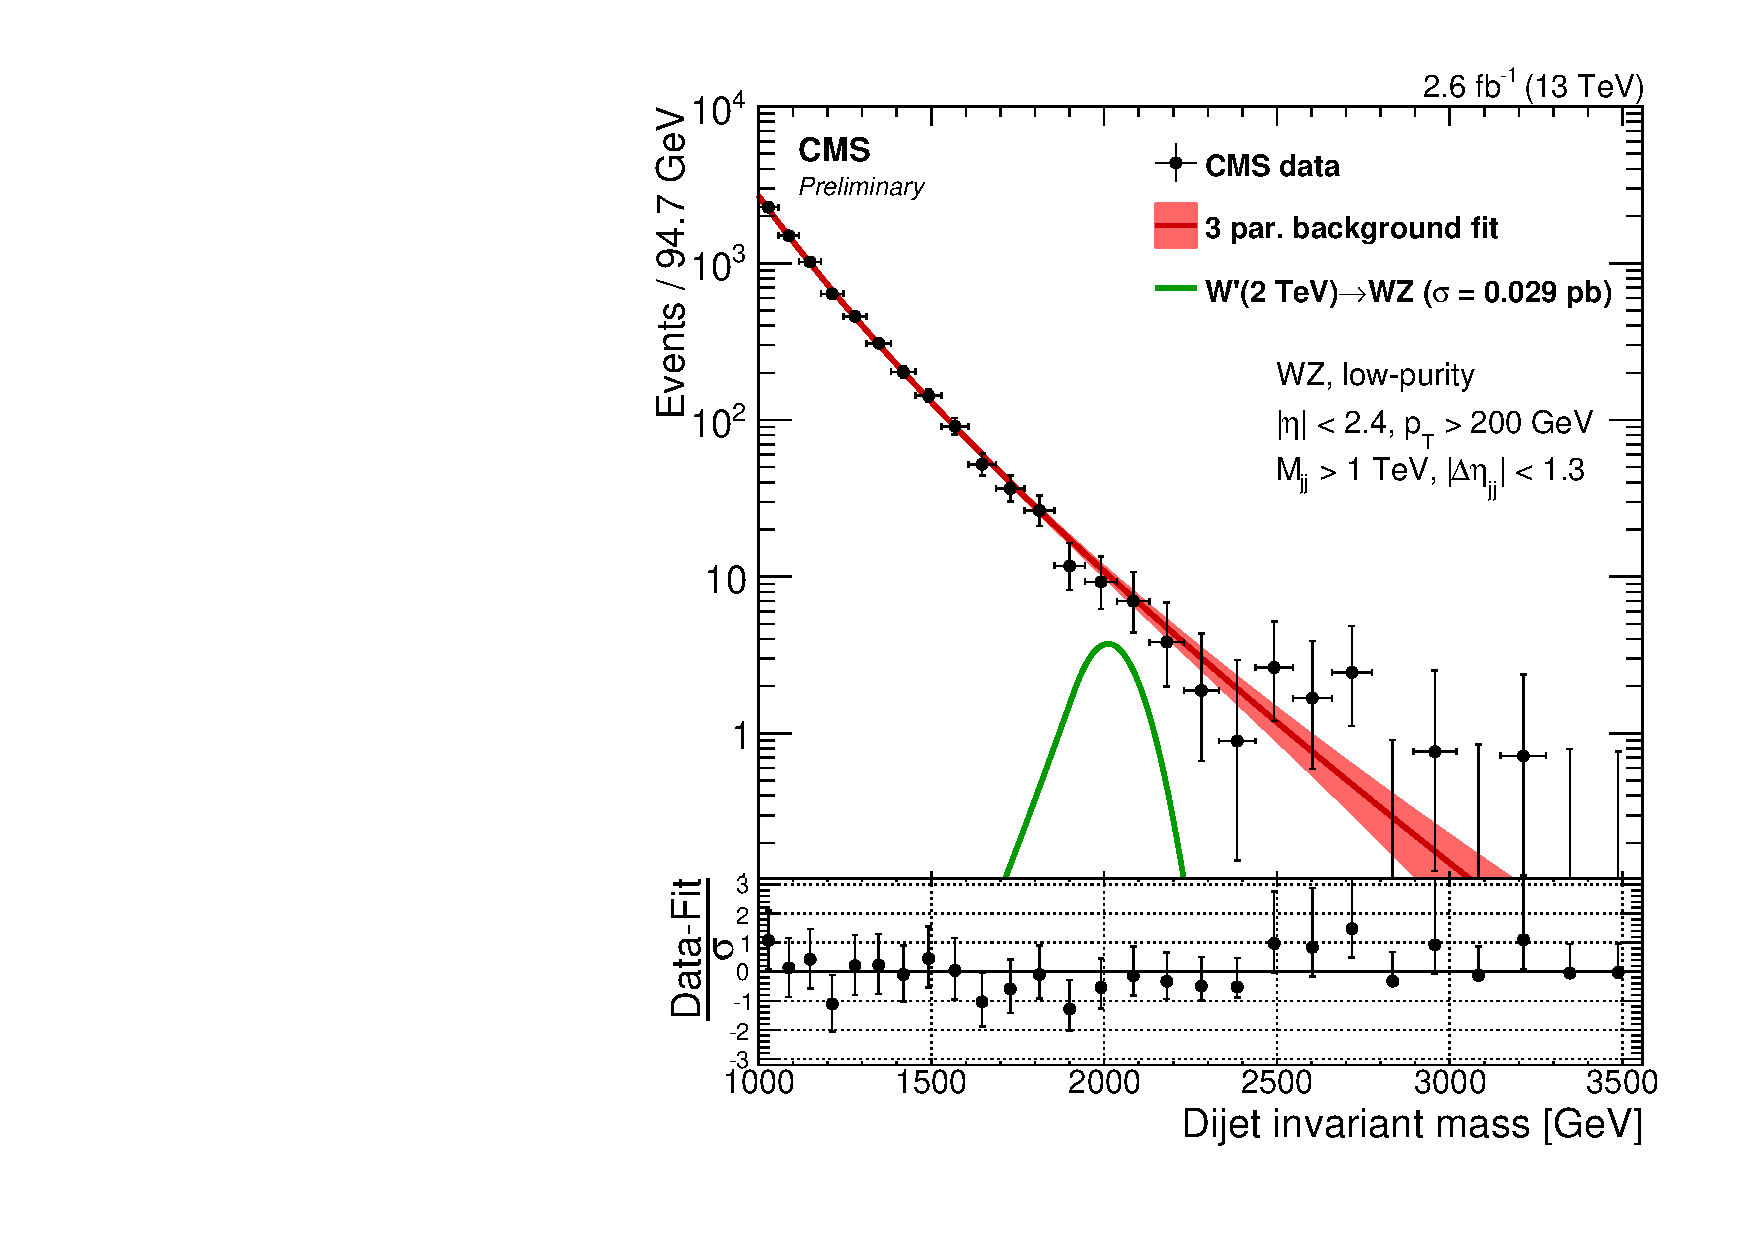
\includegraphics[width=0.44\textwidth]{figures/analysis/search1/AN-15-211/fits/MLfits/BkgFit_DijetMassLowPuriWZ.pdf}\\
\includegraphics[width=0.44\textwidth]{figures/analysis/search1/AN-15-211/fits/MLfits/BkgFit_DijetMassHighPuriZZ.pdf}
\includegraphics[width=0.44\textwidth]{figures/analysis/search1/AN-15-211/fits/MLfits/BkgFit_DijetMassLowPuriZZ.pdf}\\
\caption{Fit to data in the signal region using the background fit only for the different mass and purity categories. The filled red area correspond to the 1 sigma statistical error of the fit.}
\label{fig:search1:bkgfitMassCat}
\end{figure}

We proceed by setting limits on the cross section of the process $\text{X} \to \VV$, using the asymptotic $\textrm{CL}_\textrm{S}$ method as described in Section~\ref{sec:theory:statmet}. The binned likelihood is defined as
\begin{equation}
L = \prod_i\frac{\mu^{n_i}_ie^{-\mu_i}}{n_i!}
\end{equation}
with
\begin{equation}
\mu_i=\sigma \cdot N_i(S)+N_i(B)
\end{equation}
Here $\sigma$ is the signal strength scaling the expected number of signal events in the $i$-th dijet invariant mass bin $N_i(S)$, $N_i(B)$ is the expected number of background events in dijet invariant mass bin $i$ and $n_i$ is the observed number of events in the $ith$ dijet invariant mass bin. The background per bin $N_i(B)$ is estimated from the background component of the best signal+background fit to the data points with the signal cross section set to zero. The number of signal events in the $i$-th dijet invariant mass bin, $N_i(S)$, is then estimated from the signal templates, where only a dijet invariant mass in a 20\% window around the resonance mass is considered, containing most of the signal contribution while making sure to keep a good description of the core.
\newline
\newline
As mentioned in Section~\ref{sec:searchI:samples}, we set limits on three different signal scenarios: $\BulkG \rightarrow \WW$, $\BulkG \rightarrow \ZZ$ and $\PWpr \rightarrow WZ$. Figure \ref{fig:searchI:Limits_CombNew} shows the asymptotic limits and corresponding p-values obtained with 2.6 \fbinv of 13 \TeV CMS data after combining all mass and purity categories.

\begin{figure}[h!]
\centering
\includegraphics[width=0.32\textwidth]{figures/analysis/search1/AN-15-211/limits/brazilianFlag_BulkWW_new_combined_13TeV.pdf}
\includegraphics[width=0.32\textwidth]{figures/analysis/search1/AN-15-211/limits/brazilianFlag_WZ_new_combined_13TeV.pdf}
\includegraphics[width=0.32\textwidth]{figures/analysis/search1/AN-15-211/limits/brazilianFlag_BulkZZ_new_combined_13TeV.pdf}\\
\includegraphics[width=0.32\textwidth]{figures/analysis/search1/AN-15-211/pvalues/pvalue_BulkWWin_combined_new.pdf}
\includegraphics[width=0.32\textwidth]{figures/analysis/search1/AN-15-211/pvalues/pvalue_WZin_combined_new.pdf}
\includegraphics[width=0.32\textwidth]{figures/analysis/search1/AN-15-211/pvalues/pvalue_BulkZZin_combined_new.pdf}\\
\caption{Expected and observed limits with corresponding p-values obtained using 2.6 $\textrm{fb}^{-1}$ of CMS data after combining all mass and purity categories. Here for a Bulk $G\rightarrow WW$ (left), $W'\rightarrow WZ$ (middle) and $G\rightarrow ZZ$ (right) signal.}
\label{fig:searchI:Limits_CombNew}
\end{figure}


The statistics are too low to exclude the excess around 2 \TeV observed in the corresponding Run 1 analysis and in addition an under-fluctuation in data is present in this region. The largest excess is observed for a $\BulkG \rightarrow \ZZ$ hypothesis at a resonance mass of 2.8-3 TeV, around 2.3 $\sigma$.
This is driven by the ZZ high-purity category, the category with the lowest statictics, where one event at 3 TeV yields a local significance of 2.8 $\sigma$. A 3 parameter fit is the default background fit function for this category, however, a 2 parameter fit could also be used to describe these data. In Figure \ref{fig:searchI:Limits_ZZHP} we compare the limits and p-values obtained using a 2 parameter and a 3 parameter fit to describe the background in this category. The significance at 3 TeV is reduced from 2.8 to 1.5 $\sigma$ with a 2 parameter fit, reflecting the fact that the fit is poorly constrained in the high mass tail due to low statistics. The fit to data using both a 2 and 3 parameter fit in the ZZHP category is shown in Figure~\ref{fig:app:ZZHP2vs3p} and we in addition see that the 2 parameter fit lies within the fit uncertainties of the nominal fit.\newline
\newline

\begin{figure}[h!]
\centering
\includegraphics[width=0.49\textwidth]{figures/analysis/search1/AN-15-211/limits/brazilianFlag_BulkZZ_ZZHP_13TeV.pdf}
\includegraphics[width=0.49\textwidth]{figures/analysis/search1/AN-15-211/limits/brazilianFlag_BulkZZ_ZZHP_2parFit__13TeV.pdf}\\
\includegraphics[width=0.49\textwidth]{figures/analysis/search1/AN-15-211/pvalues/pvalue_BulkZZinZZ_high_purity.pdf}
\includegraphics[width=0.49\textwidth]{figures/analysis/search1/AN-15-211/pvalues/pvalue_BulkZZinZZ_high_purity_2par.pdf}
\caption{Expected/observed limits and corresponding p-values obtained in the ZZHP category using a 3 (left) and two (right) parameter fit to describe the background. The significance at 3 TeV is reduced from 2.8 to 1.5 $\sigma$.}
\label{fig:searchI:Limits_ZZHP}
\end{figure}

\begin{figure}[h!]
\centering
\includegraphics[width=0.49\textwidth]{figures/analysis/search1/misc/CMS-PAS-EXO-15-002_Figure_004-e.pdf}
\caption{Background fit to data in the ZZHP category using the default 3 (red) and an alternate 2 (blue) parameter fit to describe the background.}
\label{fig:app:ZZHP2vs3p}
\end{figure}


The lack of constraint on the fit in the dijet invariant mass tail when statistics are very low, is a drawback of a method relying fully on a parametric fit and reduces the analysis sensitivity in the high-\mjj region. In Search II (Section~\ref{searchII}) we will keep taking advantage of the dijet fit, however, the integrated luminosity is $\sim 15$ times higher, resulting in more datapoints in the \mjj tail which further constrains the fit. In Search III (Section~\ref{searchIII}), we will explore alternate methods which allow more control over the background shape across the full mass spectrum. 










